%% main_paper.tex
%% オートエンコーダによる多様体抽出の理論・実験的検証
%% NOLTA IEICE 日本語論文（一段組）
%% コンパイル: platex main_paper.tex && dvipdfmx main_paper.dvi
%%   または:  lualatex main_paper.tex

\documentclass[12pt,a4paper]{jsarticle}

\usepackage{amsmath,amsthm,amssymb}
\usepackage{mathtools}
\usepackage[dvipdfmx]{graphicx}
\usepackage{booktabs}
\usepackage{url}
\usepackage{here}
\usepackage{array}
\usepackage{multirow}
\usepackage[margin=25mm]{geometry}
\usepackage[dvipdfmx,hidelinks]{hyperref}

%% 定理環境（各環境で独立カウンタ — 定理は1から始まる）
\newtheorem{theorem}{定理}
\newtheorem{proposition}{命題}
\newtheorem{definition}{定義}
\newtheorem{remark}{注意}

%% 記号の略記
%% ボトルネック次元は m に統一（m := d_z）
\newcommand{\dID}{d_{\mathrm{ID}}}
\newcommand{\dz}{m}                         % ボトルネック次元（d_z = m）
\newcommand{\dzopt}{m^*}                    % 最適ボトルネック次元
\newcommand{\dtrue}{d_{\mathrm{true}}}
\newcommand{\Jg}{J_g}
\newcommand{\R}{\mathbb{R}}
\newcommand{\kap}{\kappa}
\newcommand{\AUsat}{\mathrm{AU}_{\mathrm{sat}}}
\newcommand{\dzsat}{m^{\mathrm{sat}}}       % AU飽和到達次元（明確な飽和が観測できる場合）
\newcommand{\mknee}{m^{\mathrm{knee}}}      % AU増加鈍化点（漸増型の場合）
\newcommand{\demb}{d_{\mathrm{emb}}}

\title{内在次元推定に基づくオートエンコーダの\\
       ボトルネック次元設計指針}
\author{（著者名）\\
{\small （所属機関）}\\
{\small \texttt{（メールアドレス）}}}
\date{}

\begin{document}
\maketitle

%% ===================================================================
\begin{abstract}
オートエンコーダ（Autoencoder; AE）のボトルネック次元$m$の設計は，
従来スイープや経験則に頼らざるを得ず，計算コストが高く設計根拠が不明確であった．
本論文では，内在次元（Intrinsic Dimension; ID）推定をボトルネック次元設計の指針として活用する
2段階パイプラインを提案する：
（1）大きめのボトルネック次元（$m = 256$等）で参照 AE を一度学習し，
その潜在表現に TwoNN/MLE を適用して\textbf{近似的な} ID 推定値$\hat{d}_\mathrm{ID}$を取得して候補範囲を絞り込む
（厳密な ID 推定には等長潜在空間が必要であり，参照 AE を用いる手法は実用的な近似であることに注意），
（2）VAE の AU パターン（飽和型は$m^{\mathrm{sat}}$，漸増型は$m^{\mathrm{knee}}$）を主基準として
最適ボトルネック次元$m^*$を同定する（補助基準：CKA・MSE エルボー）．
合成多様体（Swiss Roll，Torus，Möbius Band 等）および MNIST を用いた検証から，
以下の\textbf{3つの主要結果}を得た：
\begin{enumerate}
  \item \textbf{（RQ1）$\hat{d}_\mathrm{ID}$は有力な事前指標}：
        ID 推定値$\hat{d}_\mathrm{ID}$は特に合成多様体において最適ボトルネック次元と
        良好に整合し，試行錯誤を大幅に削減する有力な事前指標として機能する
        （実データでは精度が限定的な場合があることに注意が必要）．
  \item \textbf{（RQ2）$\mathrm{AU}_\mathrm{sat}$と位相的最小埋め込み次元の対応}：
        位相的に非自明な多様体（Torus，Möbius Band）において，
        VAE の AU 飽和値が位相的最小埋め込み次元と対応する傾向を観測した
        （標準化条件下；前処理依存の例外あり）．
  \item \textbf{（RQ3）IsometricAE による等長性の達成}：
        デコーダヤコビアン正則化により条件数$\kappa \approx 1$を実現し，
        潜在空間での ID 推定精度の前提条件（等長性）が達成可能であることを示した．
\end{enumerate}
副次的な発見として，MNIST における大域・局所構造形成の時間的分離を定量化した
（Epoch 5 までに Trustworthiness $\approx 0.99$，その後 TwoNN ID が漸進的増加）．
なお，本論文では接平面次元である\textbf{局所的固有次元$d_\mathrm{ID}$}と，
多様体を自己交差なく埋め込むために必要な\textbf{位相的埋め込み次元$d_\mathrm{emb}$}（$d_\mathrm{emb} \geq d_\mathrm{ID}$）を区別して用いる．
\end{abstract}

\section{まえがき}\label{sec:intro}

\subsection{研究背景}\label{sec:intro_bg}

多様体仮説（Manifold Hypothesis）\cite{fefferman2016manifold,bengio2013representation}
は，高次元データ空間$\R^N$の自然な分布が，
より低次元の滑らかな多様体$\mathcal{M}$（$\dim\mathcal{M} = d \ll N$）の周辺に
集中しているという仮定であり，
機械学習における次元削減・表現学習の理論的基盤をなす．
AE はこの多様体を潜在空間で捉えることを暗黙の目的として設計されるが，
ボトルネック次元$\dz$は通常，検証誤差の手動スイープによって決定される．
この試行錯誤は計算コストが高く，かつ設計根拠が不明確である．

\subsection{本研究の狙い}\label{sec:intro_aim}

本論文では，「データの内在次元$\dID$をあらかじめ推定し，
それをボトルネック次元の設計指針とする」という原理的アプローチを提案する．
ID 推定手法として TwoNN\cite{facco2017twonn} および MLE\cite{levina2005mle} を採用し，
その推定値と AE の最適ボトルネック次元との定量的関係を明らかにする．

\textbf{理論的背景}：この対応が成立する直感的なメカニズムを先に示す：
\begin{itemize}
  \item \textbf{AE が$\dID$を最小次元として必要とする理由}：
    データが局所的に$\dID$次元多様体に乗っている場合，
    AE が再構成誤差を有界に保つためには，データの滑らかさや AE の十分な容量などの
    条件のもとで，ボトルネック次元$m \geq \dID$が必要となることが知られている
    （定理\ref{thm:lower_bound}参照）．
    したがって$\dID$はボトルネック次元の原理的な\textbf{下界の目安}として機能し，
    TwoNN/MLE で事前に推定することでその目安を設計前に知ることができる．
  \item \textbf{VAE が$\demb$付近まで AU を活性化させる理由}：
    VAE の Gaussian 事前分布の台$\R^m$は位相的に収縮可能な空間であるため，
    基本群$\pi_1$が非自明な多様体（例：Torus；$\pi_1 = \mathbb{Z}^2$）を
    連続写像として自己交差なく潜在空間に収容するには$\demb > \dID$次元が必要となる
    （一般に滑らかな埋め込みに関する Whitney の結果等に基づく）．
    KL 正則化はこの連続写像制約の下で，十分な容量の VAE において
    最低限必要な次元$\demb$付近に AU が収束する傾向がある
    （§\ref{sec:related_topology}，命題\ref{thm:au}参照；ただし前処理・容量への依存性あり）．
\end{itemize}
すなわち，「AE は$\dID$（接空間の次元）を，VAE は$\demb$（位相的埋め込みの次元）を，
それぞれ異なる経路で近似的に反映すると考えられる」というのが本論文の中核的主張である（次節参照）．

\subsection{本論文で扱う「次元」の2種類}\label{sec:intro_dim}

本論文の議論では，多様体の「次元」として根本的に異なる2つの概念が登場する．
論理的一貫性を確保するために，ここで明確に定義しておく：

\begin{description}
  \item[局所的固有次元 $\dID$（Local Intrinsic Dimension）]
        多様体$\mathcal{M}$の各点における接平面（Tangent Space）の次元であり，
        点の近傍内での自由度を表す局所的な幾何量である．
        Swiss Roll も Torus も接平面は2次元平面であるため，等しく$\dID = 2$となる．
        TwoNN および MLE はこの局所的な距離関係から$\dID$を推定する手法である．

  \item[位相的埋め込み次元 $\demb$（Topological Embedding Dimension）]
        多様体$\mathcal{M}$を自己交差なしにユークリッド空間$\R^{\demb}$へ
        連続的に埋め込むために必要な最小次元であり，
        多様体の大域的なトポロジー構造（基本群$\pi_1$等）によって規定される
        \cite{hatcher2002algebraic,guillemin1974differential}．
        単連結多様体（$\pi_1 = \{1\}$，例：Swiss Roll）では$\demb = \dID$であるが，
        基本群が非自明な多様体（例：Torus では$\pi_1 = \mathbb{Z}^2$）では
        $\demb > \dID$となりうる（Torus の場合$\dID = 2$，$\demb = 3$）．
\end{description}

\textbf{本論文の中核的主張}：
TwoNN・MLE は局所的な距離関係を測定するため，
\textbf{本研究条件下（合成多様体および MNIST）では}$\dID$の良好な近似推定器として機能することが
経験的に確認された（ただし，有限サンプル・高曲率・クラス混合による過小評価バイアスが生じる場合あり）．
一方，VAE の$\AUsat$（AU 収束値）は，ニューラルネットワークの\textbf{連続写像という制約}のもと，
多様体を自己交差なく潜在空間に表現するために必要な次元を学習過程で「感知」するため，
\textbf{本研究条件下（位相的に非自明な合成多様体，標準化前処理）では}
後者$\demb$を近似的に反映する傾向が観測された
\cite{hatcher2002algebraic,carlsson2009topology}
（成立の目安条件：(i)正規分布事前分布，(ii)連続エンコーダ/デコーダ，
(iii)十分な容量，(iv)標準化された前処理；
実データ（MNIST 等）では未収束・前処理への依存性等の例外あり；§\ref{sec:disc_limitation}参照）．
この論理構造により，「$\dzopt \approx \hat{\dID}$（ボトルネック設計指針，RQ1）」と
「$\AUsat$が$\demb$に対応する傾向（本研究条件下での経験的観測，RQ2）」という2つの知見が，
概念的に矛盾することなく共存する．

\subsection{リサーチクエスチョン}\label{sec:intro_rq}

本論文が取り組む具体的な研究問い（Research Questions）は以下のとおりである：
\begin{description}
  \item[RQ1] TwoNN および MLE は合成多様体の$\dtrue$を本研究条件下で良好に推定できるか．
             その推定値は AE の最適ボトルネック次元$\dzopt$と，
             設計指針として有用な範囲で経験的に整合するか．
  \item[RQ2] VAE の$\AUsat$（AU 収束値，有効次元）は，本研究条件下において，多様体の位相的性質
             （基本群$\pi_1$）とどの程度の対応傾向を示すか．
             ここで$\pi_1$は損失関数に直接組み込まれるものではなく，
             $\AUsat$の解釈的枠組みとして用いる位相不変量であり，
             「多様体をユークリッド空間に連続的に埋め込む際に
             必要な最小次元（位相的最小埋め込み次元）」を規定する
             理論的指標である（§\ref{sec:discussion}参照）．
  \item[RQ3] デコーダのヤコビアン正則化によって等長埋め込みは実現可能か．
             エンコーダ側正則化（CAE）との違いは何か．
             \textbf{背景仮説}：デコーダ側の等長正則化（IsometricAE）により
             潜在空間の局所距離がデータ多様体の距離を忠実に反映するため，
             （a）TwoNN/MLE による ID 推定精度の前提条件（等長性）が保証され，
             （b）条件数$\kap \approx 1$が実現されて埋め込みの幾何学的歪みが抑制される．
             一方，エンコーダ側の正則化（CAE）はデコーダの幾何構造には直接作用しないため
             等長性の実現が困難であると予想する（実験 EC で検証）．
\end{description}

各 RQ と実験の対応は，第\ref{sec:exp}章の表\ref{tab:rq_exp_map}に整理している．

\subsection{主要貢献}\label{sec:intro_contrib}

本論文の主な貢献を以下に示す：
\begin{enumerate}
  \item \textbf{ID 推定器の系統的評価（RQ1）}：合成多様体を用いて TwoNN および MLE の
        推定精度をベンチマークし，$\hat{\dID}$が AE ボトルネック設計において
        \textbf{有力な事前指標として機能し，特に合成多様体では最適次元と良好に整合する}
        ことを実証する（実験 E1〜E3；実データでの適用には限界あり，§\ref{sec:disc_limitation}第一・第五参照）．
  \item \textbf{位相的に非自明な多様体での VAE $\AUsat$の対応傾向の観測（RQ2）}：
        Torus，Möbius Band 等の位相的に非自明な多様体において，
        変分オートエンコーダ（VAE）\cite{kingma2014vae} の$\AUsat$（AU 収束値）が
        \textbf{本研究条件下（標準化前処理，十分な収束，有限の合成多様体）では}
        位相的最小埋め込み次元と対応する傾向を経験的に観測した
        （実験 EA・EB；前処理条件・モデル容量・収束状態への強い依存性あり）．
  \item \textbf{IsometricAE による等長性の改善（RQ3）}：
        デコーダのヤコビ行列に直接正則化を加えた IsometricAE\cite{kato2020rdae,nazari2023geometric}
        が，条件数$\kap \approx 1$の等長埋め込みを実現することを示す（実験 EC）．
  \item \textbf{MNIST における構造形成の時間的分離（副次発見）}：
        MNIST の学習ダイナミクスにおいて，
        大域的近傍構造（Trustworthiness）が学習初期に急速に形成された後，
        局所的な ID が漸進的に増加するという時間的分離を定量化する（実験 E6）．
        本発見は主筋（RQ1〜RQ3）に対して補足的な知見を提供するものである．
\end{enumerate}

\subsection{本論文の構成と検証範囲の限定的な注記}\label{sec:intro_structure}

\textbf{重要：本論文における検証範囲の明示（U5）}\\
本論文の全ての定量的結果は，
（a）合成多様体（Swiss Roll，Torus，Möbius Band 等の低次元$d \leq 3$の多様体），
および（b）MNIST（全結合型 AE，$N = 784$，$d_\mathrm{ID} \approx 10$〜12）
を対象とした検証に基づくものである．
CIFAR-10 等の自然画像（畳み込み型 AE が必要），テキストデータ，時系列データ，
高解像度画像への一般化については，本論文の実験範囲外であり，
提案フレームワークの適用可能性は未検証である（§\ref{sec:disc_limitation}参照）．
読者は本論文の知見を，この限定的な検証範囲の文脈で解釈されたい．

本論文の構成は以下のとおりである：
§\ref{sec:related}（関連研究）では TwoNN/MLE の適用限界と本研究の差異を整理する．
§\ref{sec:framework}（提案フレームワーク）では2段階パイプラインと設計規則を述べる（図\ref{fig:framework_flow}）．
§\ref{sec:theory}（理論的背景）では各実験に対応する主要定理を列挙する．
§\ref{sec:exp}（実験）は（\ref{sec:exp_synthetic}）合成多様体 RQ1 実験，
（\ref{sec:exp_topology}）情報ボトルネック・位相 RQ2/RQ3 実験，
（\ref{sec:exp_mnist}）MNIST への適用，の3節で構成される．
§\ref{sec:discussion}（考察）では RQ1〜RQ3 への回答と実務ガイドラインを示す．
§\ref{sec:conclusion}（むすび）で結論を述べる．

\section{関連研究}\label{sec:related}

\subsection{内在次元推定}

内在次元推定は，高次元データが実際に占める有効次元数を推定する問題である．
TwoNN\cite{facco2017twonn} は各点の2近傍距離比$\mu_i = r_2/r_1$の
分布から内在次元を推定し，局所的な幾何構造を利用する手法として
高い精度と計算効率を有する．
MLE\cite{levina2005mle} は最尤推定の枠組みで
$k$-近傍距離の分布から次元を推定し，$k$の選択に対して安定な推定を与える．
DANCo\cite{ceruti2014danco} は角度と距離の同時分布を用いるより精密な手法だが，
計算コストが高い．
Pope ら\cite{pope2021intrinsic} は自然画像（CIFAR-10 等）の ID が
TwoNN で推定すると実際の画素次元よりはるかに低いことを示した．
なお，次元削減のための可視化・表現学習手法として広く用いられる
UMAP\cite{mcinnes2018umap} は，多様体仮説に基づく距離近似とトポロジー保存
（簡約ホモロジー\cite{chazal2021introduction}の概念に基づく）を組み合わせているが，
本研究は次元削減の可視化ではなく，ボトルネック次元の\textbf{定量的な設計指針}に焦点を当てる．
近年では，深層ニューラルネットワーク内部表現の ID 解析も進んでおり，
Ansuini ら\cite{ansuini2019intrinsic}は深層ネットワークの各層を通じて
ID が変化するパターンを定量化し，Birdal ら\cite{birdal2021intrinsic}は
永続ホモロジーと ID 推定を組み合わせた汎化誤差との関係を理論的に分析した．
Valeriani ら\cite{valeriani2023geometry}は大規模変換器モデルの隠れ表現の
幾何構造を ID の観点から系統的に解析し，層ごとに ID が先に増加してから
減少する「ハンプ」構造を報告した．

なお，TwoNN は多様体の境界付近や高曲率領域，またはサンプル数が限られた
状況において真の内在次元を\textbf{過小評価するバイアス}を持つことが
知られている\cite{facco2017twonn}．
特に$m = \dtrue$付近（過少パラメータ境界付近）での推定値は
境界効果の影響を受けやすく，$m$を真値より余裕を持って設定した条件で
推定する方が精度が高い場合がある（§\ref{sec:discussion_topology}参照）．
MNIST 等の実データへの適用においては，この過小評価バイアスを考慮した
上で推定値を解釈する必要がある．

\subsection{TwoNN/MLE の適用限界と AE ベースアプローチの必要性}\label{sec:related_topology}

TwoNN および MLE は局所的な距離関係のみを用いるため，以下の状況で精度が低下しうる．
第一に，\textbf{局所一様サンプリング仮定の破れ}：TwoNN は各点の局所近傍が
多様体上で一様にサンプリングされていることを前提とするが，
ノイズが大きい場合や多様体の曲率が高い領域では
近傍距離比$\mu_i = r_2/r_1$が真の次元とは異なる分布に従いうる\cite{facco2017twonn}．
第二に，\textbf{高次元入力空間への直接適用の困難さ}：
$N$次元入力空間（例：MNIST では$N = 784$）に直接 TwoNN を適用すると，
高次元の呪いにより局所近傍が多様体の局所構造を反映しにくくなる．
このため，AE を用いて非線形的に低次元表現を得た後に TwoNN を適用する
2段階アプローチが有効である（§\ref{sec:framework}参照）．

\textbf{VAE の Gaussian 事前分布と位相的埋め込み次元の関係：}
VAE は潜在空間に標準正規分布$\mathcal{N}(0, I_m)$を事前分布として課す．
正規分布の台$\R^m$は位相的に\textbf{収縮可能（contractible）}な空間，
すなわち任意のループを連続的に1点に変形できる空間である
\cite{hatcher2002algebraic}．
したがって，基本群$\pi_1$が非自明な多様体
（例：Torus $T^2$では$\pi_1 = \mathbb{Z}^2$）を
VAE の収縮可能な潜在空間に埋め込もうとすると，
自己交差なしには$\dID$次元の収縮可能空間には収まらず，
少なくとも$\demb > \dID$次元が必要となる
\cite{hatcher2002algebraic,guillemin1974differential}．
すなわち，VAE の KL 正則化（情報ボトルネック）が$\AUsat$を
多様体の位相的最小埋め込み次元$\demb$付近に収束させる傾向のある機構として働くと考えられる
（\textbf{ただし}，この傾向は本研究条件下（合成多様体，標準化前処理，十分な収束）で
経験的に観測されたものであり，理論的必然性は保証されていない；
有限容量・前処理条件・収束状態への強い依存性がある；
命題\ref{thm:au}，実験 EA・EB，§\ref{sec:discussion_topology}参照）．
これが，後述の実験で Torus の$\AUsat$が$\dID = 2$でなく$\demb = 3$に
対応する傾向を示す理論的背景である
（\textbf{本研究条件下での経験的傾向}；理論的な一般性は保証されておらず，
前処理・容量・収束状態に強く依存する点に注意）．

\textbf{等長性（$\kap$）と Trustworthiness の微分幾何学的関係：}
条件数$\kap = \sigma_1/\sigma_m$（デコーダヤコビアン$\Jg$の最大・最小特異値比）は，
デコーダが局所的に距離を均等に伸縮する度合いを測る微分幾何学的指標である．
$\kap = 1$（等長埋め込み）が成立するとき，プルバック計量$G = \Jg^\top\Jg \propto I_m$となり，
潜在空間の無限小距離が元空間の無限小距離と等価になる
（定理\ref{thm:pullback}）．
一方，Trustworthiness は有限$k$-近傍ランクの大域的な保存を測る指標であり，
$\kap \approx 1$（局所的距離保存）はその\textbf{微分幾何学的な精密版}に相当する：
$\kap \approx 1$が保証されれば，局所的距離関係が歪みなく保存されるため，
近傍ランクの保存（Trustworthiness 改善）が局所スケールでも保証されるからである
（実験 EC，§\ref{sec:discussion_topology}参照）．

\subsection{AE のボトルネック次元と表現品質}

$\beta$-VAE\cite{higgins2017betavae} は KL 正則化の重みを大きくすることで
disentangled な潜在表現を促進する．
Lucas ら\cite{lucas2019elbo} は ELBO の最小化において
posterior collapse（AU の大幅な減少）が生じる条件を線形 VAE の枠組みで分析し，
AU が $d_{\mathrm{ID}}$ 近傍で飽和することを理論的に示した．
ただし，Lucas ら\cite{lucas2019elbo} の知見は単一の線形多様体を前提とした分析であり，
\textbf{位相的に非自明な多様体（Torus，Möbius Band 等）において AU が
位相的最小埋め込み次元$\demb$付近に収束するという対応傾向について，
本研究条件下（標準化前処理，十分な収束）での経験的観測を行った}
（実験 EA・EB；ただし条件依存性が強く，理論的必然性は保証されていない）．

Nazari ら\cite{nazari2023geometric} は幾何的オートエンコーダを提案し，
エンコーダが多様体の幾何構造を歪めずに保存するための正則化を導入した．
Kato ら\cite{kato2020rdae} および Nazari ら\cite{nazari2023geometric} は，
デコーダのヤコビ行列$\Jg(z) \in \R^{N \times m}$に対して
プルバック計量$G(z) = \Jg(z)^\top \Jg(z)$を単位行列に近づける正則化項を用いる
IsometricAE を提案した．その損失関数は
\begin{equation}
  \mathcal{L}_{\mathrm{iso}} = \mathcal{L}_{\mathrm{rec}}
  + \lambda_{\mathrm{iso}} \cdot \frac{1}{n}\sum_{i=1}^{n}
    \|\Jg(z_i)^\top \Jg(z_i) - I_m\|_F^2
  \label{eq:iso_loss}
\end{equation}
と表され，$\lambda_{\mathrm{iso}}$は等長正則化の重みである
（本実験では$\lambda_{\mathrm{iso}} = 0.01$を用いる；§\ref{sec:exp_setup}参照）．
条件数$\kap = \sigma_1/\sigma_m$（最大・最小特異値比）が 1 に近づくほど
デコーダが等長埋め込みに近くなる．
\textbf{本研究における IsometricAE の独自点}：Nazari ら\cite{nazari2023geometric} および
Kato ら\cite{kato2020rdae} の等長正則化は，主に潜在表現の可視化や下流タスクの
精度向上を目的としているのに対し，本研究では「等長性が TwoNN/MLE による
ID 推定精度の前提条件であること」を明確化し，ボトルネック次元設計パイプラインにおける
ID 推定の信頼性検証ツールとして位置づける点が本質的に新しい．
また，本研究ではエンコーダ側正則化（CAE）との比較実験を通じて，
等長性の実現にはデコーダ側の正則化が不可欠であることを実証する（実験 EC，§\ref{sec:disc_rq3}）．

収縮型 AE（CAE）\cite{rifai2011cae} はエンコーダのフロベニウスノルムを
罰則化することで入力の局所変化に不変な特徴を学習する．
デノイジング AE（DAE）\cite{alain2014dae} は加算雑音入力から
クリーンな出力を予測することでスコア関数を暗黙的に推定し，
多様体の接空間方向に選択的な表現を学習することが理論的に知られている．

\subsection{本研究との差異}

既存研究の多くは単一の評価指標に基づく AE の性能評価にとどまり，
ID 推定とボトルネック次元設計を系統的に結びつけた研究は少ない．
本研究は ID 推定・AU・CKA・条件数$\kap$・Trustworthiness を
統合した多指標評価パイプラインを構築し，
合成多様体と実データ（MNIST）の双方で$\dzopt \approx \hat{\dID}$を実証する点で
既存研究と一線を画する．
また，既存研究では TwoNN の過小評価バイアス（§\ref{sec:related}参照）を
明示的に考慮した上でのボトルネック設計指針が示されておらず，
本研究はこの点についても批判的な考察を提供する（§\ref{sec:discussion_topology}参照）．

なお，本研究でいう「多指標統合」は，各指標を同列に混合することではなく，
\textbf{(i) AU 飽和により$\dzopt$の候補集合を定め（モデル選択の主基準），
(ii) CKA・MSE・Trustworthiness を用いて候補間の優劣や例外を検証する（補助基準）}
という役割分担に基づく．この選択規則を 3.1 節に明示することで，
提案手法の再現可能性を担保する．

\section{提案フレームワーク}\label{sec:framework}

本論文ではボトルネック次元を一貫して$m$（$:= d_z$）で表記し，探索グリッド上の具体的な次元値も$m$を用いる．最適ボトルネック次元は$m^*$，AU 飽和到達次元は$m^{\mathrm{sat}}$と表記する．

\subsubsection*{主要記号一覧}
\begin{table}[H]
\centering
\caption{本論文で使用する主要記号}
\label{tab:notation}
\small
\begin{tabular}{lll}
\toprule
記号 & 意味 & 関連節 \\
\midrule
$m$（$= d_z$） & AE のボトルネック次元（設計パラメータ） & §\ref{sec:framework} \\
$\dzopt$（$= m^*$） & 最適ボトルネック次元 & §\ref{sec:framework} \\
$\dzsat$（$= m^{\mathrm{sat}}$） & AU 飽和が最初に到達する次元（飽和型） & 式\eqref{eq:dzopt_sat} \\
$\mknee$（$= m^{\mathrm{knee}}$） & AU 増加率が鈍化する屈曲点次元（漸増型） & 式\eqref{eq:dzopt_knee} \\
$\AUsat$ & AU がグリッド上で到達する最大活性ユニット数 & 式\eqref{eq:dzopt_sat} \\
$\mathrm{AU}(m)$ & ボトルネック次元$m$での活性ユニット数 & §\ref{sec:framework} \\
$\hat{\dID}$ & TwoNN/MLE による内在次元の推定値 & §\ref{sec:framework} \\
$\dtrue$ & 合成多様体の真の内在次元（既知） & §\ref{sec:exp_synthetic} \\
$\demb$ & 位相的最小埋め込み次元（$\demb \geq \dID$） & §\ref{sec:intro_dim} \\
$\kap$ & デコーダヤコビアンの条件数（等長性の指標） & §\ref{sec:related_topology} \\
$r(m)$ & AU の正規化増加率 & 式\eqref{eq:au_rate} \\
$\tau_{\mathrm{knee}}$ & 漸増型の屈曲点検出閾値（本研究では 0.25） & 式\eqref{eq:dzopt_knee} \\
\bottomrule
\end{tabular}
\end{table}

\subsection{2段階パイプライン}

本研究が提案するフレームワークは以下の2段階から構成される．

\textbf{Stage 1：ID 推定器の評価・選択}

真の$\dtrue$が既知の合成多様体（Swiss Roll，Torus 等）を用いて
TwoNN と MLE の推定精度をベンチマークし，信頼できる推定器を選択する．

\textbf{Stage 2：ID とボトルネック次元の関係分析}

ボトルネック次元$\dz$を離散グリッド
$\mathcal{M} = \{1, 2, 4, 8, 12, 16, 20, 32, 64, 128, 256\}$上でスイープし，
各設定で AE/VAE を学習する．

\begin{remark}[離散グリッドの解像度と$\dzopt$の精度]\label{rem:grid_resolution}
$\mathcal{M}$は対数スケールに近い離散グリッドであるため，
真の$\dID$がグリッド間（例：$\dID = 6$が$m=4$と$m=8$の間）に位置する場合，
$\dzopt$を$\dID$と完全に一致させることはできない．
このような場合，$r(m)$の変化点（AU が$\dID$を初めて超えるグリッド点）が
$\dzopt$の保守的な上界として機能する（例：$\dID = 6$なら$m = 8$が設計目安）．
実務上は，$\hat{\dID}$付近の密なグリッド（例：$m \in \{4,5,6,7,8\}$）で追加確認することが推奨される．
本論文の実験では合成多様体の$\dID \in \{2\}$，MNIST の$\dID \approx 10$〜12 がいずれも
グリッド点（$m = 2, 8, 12$等）と一致する設定であるため，
この解像度問題による誤差は最小化されている．
\end{remark}

\begin{figure}[H]
\centering
\renewcommand{\arraystretch}{1.5}
\begin{tabular}{c}
  \fbox{\textbf{入力データ} $\boldsymbol{X} \in \R^N$} \\[4pt]
  $\Big\downarrow$ \\[2pt]
  \fbox{\parbox{0.72\linewidth}{\centering
    \textbf{Stage 1：内在次元の推定（TwoNN / MLE）}\\[2pt]
    低次元合成多様体（$\dtrue$既知）でベンチマーク → 推定器を選択\\
    実データには AE（$m_{\mathrm{ref}} \gg \hat{\dID}$）の潜在空間経由で適用\\
    $\Rightarrow$ 推定値 $\hat{\dID}$ を取得
  }} \\[4pt]
  $\Big\downarrow$ \quad（$\hat{\dID}$をボトルネック設計の指針として利用）\\[2pt]
  \fbox{\parbox{0.72\linewidth}{\centering
    \textbf{Stage 2：最適ボトルネック次元の探索（VAE スイープ）}\\[2pt]
    $m \in \mathcal{M} = \{1,2,4,8,12,16,20,32,64,128,256\}$ でスイープ\\
    各 $m$ で VAE（$\beta=4$）を学習 → AU($m$) を計算\\
    AU パターン判別（式\eqref{eq:dzopt}）$\Rightarrow$
    飽和型：$\dzopt = \dzsat$，漸増型：$\dzopt = \mknee$\\
    補助基準：CKA・MSE エルボーで$\dzopt$を確定（式\eqref{eq:dzopt_cka}/\eqref{eq:dzopt_cka_knee}）
  }} \\[4pt]
  $\Big\downarrow$ \quad（前提条件の検証・補助実験）\\[2pt]
  \fbox{\parbox{0.72\linewidth}{\centering
    \textbf{IsometricAE：潜在空間 ID 推定精度の前提条件検証（RQ3）}\\[2pt]
    デコーダヤコビアン$\Jg$に正則化（式\eqref{eq:iso_loss}）\\
    $\Rightarrow \kap \approx 1$（等長性）を確認\\
    等長性が成立するとき，潜在空間での TwoNN/MLE は最も信頼できる
  }}
\end{tabular}
\caption{提案フレームワークのデータフロー．
Stage 1 で $\hat{\dID}$ を推定し，Stage 2 の VAE ボトルネック探索の指針とする．
IsometricAE（RQ3）は，潜在空間での ID 推定精度に必要な
等長性条件が実現可能であることを検証する補助実験として位置づける．}
\label{fig:framework_flow}
\end{figure}

\begin{remark}[実データへの適用における ID 推定の循環性と等長性バイアスについて]\label{rem:circularity}
MNIST のような入力次元$N$が大きいデータでは，入力空間に直接 TwoNN を適用すると
計算コストが高く，かつ高次元の呪いにより精度が低下しやすい（$N = 784$の場合，
局所近傍が多様体の局所構造を反映しにくくなる）．
本研究では，大きめのボトルネック次元（$m = 256$）で標準 AE を\textbf{一度だけ}事前学習し，
その低次元潜在表現上で TwoNN/MLE を適用することで ID を推定する方法を採用した
（§\ref{sec:exp_mnist}参照）．

\textbf{等長性バイアスに関する理論的注意点：}
この参照 AE（標準 AE，$m = 256$）は等長正則化を施していないため，
条件数$\kap > 1$（実験 EC の標準 AE で$\kap = 1.433\pm0.182$，$m = 2$の場合）の
歪んだ潜在空間を形成する可能性がある．
理論的には，$\kap > 1$の潜在空間では TwoNN/MLE の局所距離仮定が厳密には成立せず，
推定された$\hat{\dID}$にバイアスが生じるリスクがある．
理想的には IsometricAE（$\kap \approx 1$）を参照 AE として用いるべきであるが，
これはボトルネック次元$m$を事前に知る必要があるため，鶏と卵の問題（chicken-and-egg）が生じる．

\textbf{実証的な緩和策：}
本研究では以下の経験的証拠によりこのバイアスが実用上許容範囲内であることを示す：
（a）表\ref{tab:e4_ae}に示すとおり，$m \geq 64$ の複数グリッド点で
TwoNN ID（9.54〜10.02）および MLE ID（11.26〜11.85）が収束していること
（複数$m$での一致は，歪みによるバイアスが系統的に一方向に偏っていないことを示唆する）；
（b）標準 AE の$m = 256$での条件数は$m = 2$の場合より有意に低い可能性がある
（大きな$m$では情報ボトルネックが緩和され，等長性に近くなる傾向が期待される）．
ただし，この緩和策は経験的なものであり，参照 AE の等長性が MNIST の設定で
完全に保証されているわけではない（§\ref{sec:disc_limitation}第十一を参照）．

この手順は一見循環して見えるが，この事前学習は設計指針取得のための
\textbf{一回限りの参照ステップ}であり，
得られた$\hat{\dID}$を指針として$\dzopt \approx \hat{\dID}$となる最終モデルを別途設計する．
この2ステップ運用により，最終的には$m \ll N$の軽量なモデルで設計を完了できる．
\textbf{要約}：本手法は完全な非循環ではないが，複数$m$での ID 推定値の収束という経験的緩和策を経ることで，実用上は問題のない近似として機能する．
\end{remark}
最適ボトルネック次元$\dzopt$は，\textbf{VAE の AU パターン}（飽和型か漸増型か）に応じて
以下のようにケース分けして定める．$\dz$は離散探索グリッド
$\mathcal{M} = \{1, 2, 4, 8, 12, 16, 20, 32, 64, 128, 256\}$から選ばれる整数値である．

まず，AU の正規化増加率を
\begin{equation}
  r(m) = \frac{\mathrm{AU}(m) - \mathrm{AU}(m_{\mathrm{prev}})}{m - m_{\mathrm{prev}}}
  \label{eq:au_rate}
\end{equation}
と定義する（$m_{\mathrm{prev}}$は$\mathcal{M}$上の直前のグリッド点）．
$r(m) = 1$はすべての潜在次元が利用されていることを，$r(m) \approx 0$は
KL 正則化が追加次元を抑制していることを意味する．

\textbf{AU パターンの判別}：
\begin{itemize}
  \item \textbf{飽和型}：$\mathcal{M}$内の連続する2点以上で AU が同一値を維持する
        （プラトー幅 $\geq 2$），すなわち$\exists m_0 \in \mathcal{M}$で
        $\mathrm{AU}(m_0) = \mathrm{AU}(m_0') \;(m_0' > m_0)$が成立する場合．
        \textit{典型例：Swiss Roll，Torus}（VAE の KL 正則化が明確な次元選択を行う）．
  \item \textbf{漸増型}：$\mathrm{AU}(m)$がグリッド全体にわたってほぼ単調増加し，
        $\mathrm{AU}(m_{\max}) \approx \AUsat$が最大$m$にのみ現れる場合．
        \textit{典型例：MNIST}（多クラス混合分布のため AU が緩やかに増加し続ける）．
\end{itemize}

\textbf{最適ボトルネック次元のケース別定義}：
\begin{equation}
  \dzopt =
  \begin{cases}
    \dzsat \;\coloneqq\; \min\bigl\{m \in \mathcal{M} \;\big|\; \mathrm{AU}(m) = \AUsat\bigr\}
      & \text{（飽和型，式\eqref{eq:dzopt_sat}）} \\[4pt]
    \mknee \;\coloneqq\; \min\bigl\{m \in \mathcal{M} \;\big|\; r(m) < \tau_{\mathrm{knee}}\cdot r_{\max}\bigr\}
      & \text{（漸増型，式\eqref{eq:dzopt_knee}）}
  \end{cases}
  \label{eq:dzopt}
\end{equation}
ここで，
\begin{align}
  \AUsat &= \max_{m' \in \mathcal{M}} \mathrm{AU}(m'), \label{eq:dzopt_sat} \\
  r_{\max} &= \max_{m' \in \mathcal{M}} r(m'), \quad
  \tau_{\mathrm{knee}} \in (0,1) \text{（本研究では } \tau_{\mathrm{knee}} = 0.25\text{）．} \label{eq:dzopt_knee}
\end{align}
$\mknee$は AU の増加率が最大増加率の$\tau_{\mathrm{knee}}$倍を下回る最小次元，
すなわち KL 正則化による次元圧縮が初めて顕現する屈曲点である．
MNIST VAE では，$m=8 \to 12$間の正規化増加率$r(12) = 0/4 = 0.0$が
$0.25 \cdot r_{\max} = 0.25$を下回るため$\mknee = 12$と同定される．

\textbf{$\tau_{\mathrm{knee}}$の根拠（概要）：}

$r(m)$は，ボトルネック次元の追加で VAE が獲得する「情報的自由度」の限界効用と解釈できる
（情報ボトルネック理論\cite{tishby2000ib}参照）．
$\tau_{\mathrm{knee}} = 0.25$は以下の2つの根拠を持つ経験的設定値である：
（1）\textbf{感度的頑健性}：全データセット（Swiss Roll，Torus，MNIST）で
$\tau \in [0.1, 0.5]$の範囲内で$\mknee$の同定結果が不変であることを確認した；
（2）\textbf{情報理論的動機}：AU$(m) \approx A(1-e^{-\alpha m})$の指数飽和モデルのもとで
$\tau = 0.25$は理論的屈曲領域$[0.25,\, e^{-1}]$の保守的下界に対応する．
詳細な感度分析と指数モデルの導出は付録\ref{app:tau_knee}を参照されたい．
なお，$r(m)$が全グリッドで高い値を維持する飽和型データは漸増型判別に該当せず，
$\tau_{\mathrm{knee}}$は参照されない．

\textbf{閾値依存性を低減するデータ駆動的代替：}
$r(m)$が 0.3〜0.7 の範囲を緩やかに低下するデータセットでは，
閾値に依存しない代替手段として$r(m)$の二階差分が最大となる点を用いることができる：
\begin{equation}
  m^{\mathrm{knee},\Delta^2} = \arg\max_{m \in \mathcal{M} \setminus \{m_{\min}, m_{\max}\}}
  \Delta^2 r(m), \quad
  \Delta^2 r(m) \coloneqq r(m_{\mathrm{next}}) - 2r(m) + r(m_{\mathrm{prev}})
  \label{eq:knee_curvature}
\end{equation}
（$m_{\mathrm{prev}}, m_{\mathrm{next}}$は$\mathcal{M}$上の前後のグリッド点）．

実用的な判断の優先順位：
(1) $r(m)$にステップ型の明確な不連続がある場合：$\tau_{\mathrm{knee}} \in [0.1, 0.5]$で$\mknee$は安定；
(2) $r(m)$が緩やかに低下する場合：式\eqref{eq:knee_curvature}の$m^{\mathrm{knee},\Delta^2}$を優先し，
CKA プラトー（式\eqref{eq:dzopt_cka_knee}）で最終確認；
(3) 不明瞭な境界的ケースでは CKA プラトーが最終判断を担う．
$\mknee$はあくまで実用的な設計目安であり，補助基準（CKA）で最終決定を行う（後述の設計規則参照）．

\paragraph{閾値 $\tau_{\mathrm{knee}}$ の位置づけ}
本研究では，漸増型データにおける鈍化点の検出のために $\tau_{\mathrm{knee}}=0.25$ を用いた．
この値は，情報ボトルネット的な指数飽和の直観（上記の根拠 2）および
本研究で扱ったデータセット（Swiss Roll，Torus，MNIST）上での感度分析に基づいて採用したものであるが，
あらゆるデータセットに対して普遍的に最適であることを主張するものではない．

$\tau_{\mathrm{knee}}=0.25$ は本研究の実験条件において有効であった
\textbf{経験的設定値}として位置づけるのが適切であり，
他の画像データ，自然言語データ，時系列データなどへ適用する際には，
二階差分に基づくデータ駆動的な代替基準（式\eqref{eq:knee_curvature}）と併用しつつ
再調整することが望ましい（§\ref{sec:disc_limitation}第六参照）．

ここで，本論文全体にわたって使用する3つの概念を明確に区別する：
\begin{description}
  \item[$\AUsat$（AU飽和値）] VAE の AU がグリッド$\mathcal{M}$上で到達する
        \textbf{最大活性ユニット数}（式\eqref{eq:dzopt_sat}）．
        多様体の実効次元や位相的最小埋め込み次元を反映する指標として用いる．
        漸増型では最大$m$でのみ達成され，飽和型では複数点で維持される．
  \item[$\dzsat$（AU飽和到達次元）] \textbf{飽和型}において AU が$\AUsat$に達する
        グリッド上の最小ボトルネック次元（式\eqref{eq:dzopt}，飽和型のケース）．
        合成多様体のように AU が急激に飽和する場合に$\dzopt = \dzsat$として採用する．
  \item[$\mknee$（AU 鈍化点）] \textbf{漸増型}において AU の正規化増加率$r(m)$が
        著しく低下する最初の屈曲点（式\eqref{eq:dzopt}，漸増型のケース）．
        $\AUsat$（最終的な最大 AU 値）とは数値上も概念上も異なる．
        MNIST では$\mknee = 12$（$\AUsat = 36$）．
\end{description}

\textbf{位相との対応は$\AUsat$を用いる}：
EB 実験（§\ref{sec:exp_eb}）および考察（§\ref{sec:discussion_topology}）では，
多様体の位相的最小埋め込み次元と$\AUsat$（AU の収束値）が対応することを議論する．
これはあくまで「潜在表現が有効に使っている次元数」の話であり，
「いくつの$\dz$でモデルを設計するか」という$\dzsat$（設計変数）の話とは区別される．

\textbf{設計規則：$\dzopt$ の決定手順（2分岐）}

式\eqref{eq:dzopt}のケース判別後，補助基準（CKA・MSE）で$\dzopt$を確定する：

\medskip
\noindent\underline{\textbf{【飽和型】$\dzopt = \dzsat$を採用する場合}}
\begin{enumerate}
  \item \textbf{候補集合の定義}：AU が飽和している次元集合
        $\mathcal{C}_{\mathrm{sat}} = \{m \in \mathcal{M} \mid \mathrm{AU}(m) = \AUsat\}$を求める．
  \item \textbf{CKA による最小次元選択}：$\mathcal{C}_{\mathrm{sat}}$の中で CKA が
        最大値に十分近い最小次元を$\dzopt$とする：
        \begin{equation}
          \dzopt = \min\!\left\{m \in \mathcal{C}_{\mathrm{sat}}
          \;\middle|\;
          \mathrm{CKA}(m) \geq (1-\varepsilon)\max_{m'\in\mathcal{C}_{\mathrm{sat}}}\mathrm{CKA}(m')
          \right\}
          \label{eq:dzopt_cka}
        \end{equation}
        ここで$\varepsilon = 0.01$（本研究値；本実験全体で CKA の変動幅が最大 2〜3\% に
        収まることを確認）．
  \item \textbf{MSE 肘点の整合確認}：MSE 肘点$m^*_{\mathrm{elbow}}$（式\eqref{eq:elbow_def}）が
        $\dzopt$と大きく乖離しないことを補助的に確認する．
\end{enumerate}

\medskip
\noindent\underline{\textbf{【漸増型】$\dzopt = \mknee$を採用する場合}}
\begin{enumerate}
  \item \textbf{$\mknee$の同定}：式\eqref{eq:dzopt}（漸増型）で$\mknee$を算出する．
        MNIST では$\mknee = 12$．
  \item \textbf{CKA プラトーとの照合}：$\mknee$付近で CKA の増加が鈍化する
        （プラトーに入る）ことを確認し，候補範囲を$\mathcal{C}_{\mathrm{knee}}
        = \{m \in \mathcal{M} \mid m \geq \mknee,\; r(m) < \tau_{\mathrm{knee}} \cdot r_{\max}\}$とする．
        式\eqref{eq:dzopt_cka}と同じ$\varepsilon$基準で最小次元を$\dzopt$とする：
        \begin{equation}
          \dzopt = \min\!\left\{m \in \mathcal{C}_{\mathrm{knee}}
          \;\middle|\;
          \mathrm{CKA}(m) \geq (1-\varepsilon)\max_{m'\in\mathcal{C}_{\mathrm{knee}}}\mathrm{CKA}(m')
          \right\}
          \label{eq:dzopt_cka_knee}
        \end{equation}
  \item \textbf{$\AUsat$との混同を避ける}：$\dzopt$（設計すべきボトルネック次元）と
        $\AUsat$（最終的な最大 AU 値）は別概念であり，漸増型では$\dzopt \ll \AUsat$となりうる
        （MNIST 例：$\dzopt \approx 12$〜16，$\AUsat = 36$）．
\end{enumerate}

\noindent\textbf{統一的な見方：}\textbf{AU パターンにかかわらず}，\textbf{AU を主基準，
CKA を補助基準，MSE を整合確認}とすることで，「最小次元で情報次元の利用効率が飽和
（または屈曲）し，かつ表現類似度が十分高い」設計点を一貫した手順で同定できる．

AU 飽和を主要基準として採用する理由は，その情報理論的な客観性にある．
AIC や BIC のような情報量基準はパラメータ数のペナルティ項を必要とし，
AE のような非線形モデルでは有効パラメータ数の定義が自明でない．
これに対し AU 飽和は，KL 正則化（情報ボトルネック制約）のもとで
モデルが\textbf{実際に使用している情報次元}を直接測定する客観的指標であり，
モデル選択問題に対して AIC/BIC とは独立したデータ駆動的な解を与える
（命題\ref{thm:au}参照）．
さらに，MNIST のように MSE 曲線が滑らかになる（Smooth elbow problem）
複雑なデータセットにおいても AU 飽和は客観的に検出可能である．

\textbf{補助的指標としての MSE エルボー（平滑化付き）：}
テスト再構成誤差
\begin{equation}
  \mathcal{L}(\dz) = \frac{1}{n_{\mathrm{test}}}
  \sum_{i=1}^{n_{\mathrm{test}}} \|\boldsymbol{x}_i - g(f(\boldsymbol{x}_i))\|^2
  \label{eq:mse_def}
\end{equation}
の推移は AU 飽和の補助的な確認手段として用いる．
確率的勾配降下法（SGD）による学習のばらつき等により
MSE 曲線に微小なノイズが乗っている場合，
二次差分を直接適用すると偽のエルボーを検出する恐れがある．
そこで，まず移動平均（ウィンドウ幅$w$）による\textbf{事前平滑化}を行う：
\begin{equation}
  \tilde{\mathcal{L}}(m_k) = \frac{1}{2w+1}\sum_{j=-w}^{w}\mathcal{L}(m_{k+j})
  \label{eq:mse_smooth}
\end{equation}
（端点では利用可能な点のみを平均する．本研究では$w=1$，すなわち3点移動平均を用いる．）
平滑化後の MSE に対して正規化二次差分を計算し，
\begin{equation}
  \Delta^2(m_k) = \frac{\tilde{\mathcal{L}}(m_{k-1}) - 2\tilde{\mathcal{L}}(m_k) + \tilde{\mathcal{L}}(m_{k+1})}
                        {\tilde{\mathcal{L}}(m_1)}
  \label{eq:elbow}
\end{equation}
が最大となる点をエルボー点とする：
\begin{equation}
  m^*_{\mathrm{elbow}} = \arg\max_{k \in \{2,\ldots,K-1\}} \Delta^2(m_k)
  \label{eq:elbow_def}
\end{equation}
この平滑化は，ノイズに起因する偽エルボーを抑制し，
二次差分の検出安定性を補強する役割を持つ．

\textbf{平滑化の効果の定量的確認：}
合成多様体（Swiss Roll，Torus）では MSE の肘点が急峻である（Swiss Roll の$m=1 \to 2$で
約 34 倍の急落）ため，$w=0$（無平滑化）でも$w=1$でも二次差分の最大点が
$m = \dtrue$と正確に一致し，検出精度に差は生じない．
一方 MNIST では，$w=0$・$w=1$のいずれでも正規化二次差分$\Delta^2(m)$が
全グリッドで単調に微小値をとり（最大値$\Delta^2 < 0.05$），
明確なエルボー点を抽出できない（図\ref{fig:e4}参照）．
したがって，移動平均はノイズへの頑健性を保証する設計上の安全弁であるが，
MNIST の Smooth elbow problem の本質的な解決策ではなく，
そのような複雑なデータでは AU を主基準とする手順（式\eqref{eq:dzopt}，式\eqref{eq:dzopt_cka_knee}）が
主線となる（MSE エルボーは補助的確認にとどまる）．

\subsection{評価指標}

\textbf{TwoNN 内在次元推定量}\cite{facco2017twonn}：
各サンプル$\boldsymbol{x}_i$の最近傍距離$r_1$と2番目の近傍距離$r_2$の比
$\mu_i = r_2/r_1$を用い，
\begin{equation}
  \hat{\dID}^{\mathrm{TwoNN}} = \frac{1}{\mathbb{E}[\log \mu_i]}
\end{equation}
により内在次元を推定する．

\textbf{MLE 内在次元推定量}\cite{levina2005mle}：
$k$-近傍距離の対数比から最尤推定量を構成する：
\begin{equation}
  \hat{\dID}^{\mathrm{MLE}} = \left[
    \frac{1}{k-1}\sum_{j=1}^{k-1}\log\frac{r_k(\boldsymbol{x}_i)}{r_j(\boldsymbol{x}_i)}
  \right]^{-1}
\end{equation}

\textbf{活性ユニット数（AU）}\cite{lucas2019elbo}：
VAE の潜在次元$k$が活性かどうかを，
入力$\boldsymbol{x}$に対する事後平均の分散で判定する．
$V_k = \mathrm{Var}_{\boldsymbol{x}}[\mathbb{E}_{q_\phi}[z_k|\boldsymbol{x}]]$
とおくとき，
\begin{equation}
  \mathrm{AU} = \sum_{k=1}^{\dz}
  \mathbf{1}\bigl[V_k > \delta\bigr],
  \quad \delta = 10^{-2}
  \label{eq:au}
\end{equation}
ここで$\delta = 10^{-2}$は文献\cite{lucas2019elbo}の標準値である．
本論文の全実験はこの絶対閾値で統一して実施しており，
感度分析として$\delta \in \{10^{-3}, 10^{-2}, 5\times10^{-2}, 10^{-1}\}$での
主要結論の変化を確認済みである（§\ref{sec:exp_setup}参照）．

\begin{remark}[$\delta$のデータスケール依存性について]
$\delta = 10^{-2}$は絶対値であり，データスケールが大きく異なる実データでは
適切でない場合がある（例：医用画像でピクセル値が0〜255の場合）．
汎用的な運用では，$\delta_\mathrm{rel} = \rho \cdot \max_{k'} V_{k'}$（$\rho = 10^{-2}$）
のように観測された最大分散を基準とする相対閾値が望ましい．
標準正規事前分布（$\max_{k'} V_{k'} \approx 1$）のもとでは$\delta_\mathrm{rel} \approx 0.01$となり，
本実験と数値的に整合する．本論文の実験設定（入力 [0,1] 正規化）では
この違いは結果に実質的な影響を与えないため，文献値の絶対閾値を採用した．
\end{remark}

\textbf{Centered Kernel Alignment（CKA）}\cite{kornblith2019cka}：
入力$\boldsymbol{X} \in \R^{n \times N}$と再構成$\hat{\boldsymbol{X}} \in \R^{n \times N}$の
表現類似度を測る指標である．
本研究では線形カーネルを用い，カーネル行列を
$K = \boldsymbol{X}\boldsymbol{X}^\top \in \R^{n \times n}$，
$L = \hat{\boldsymbol{X}}\hat{\boldsymbol{X}}^\top \in \R^{n \times n}$
と定義する（$n$はサンプル数）．センタリング行列
$H = I_n - \frac{1}{n}\boldsymbol{1}\boldsymbol{1}^\top$
を用いて，CKA を
\begin{equation}
  \mathrm{CKA}(K, L)
  = \frac{\mathrm{HSIC}(K, L)}{\sqrt{\mathrm{HSIC}(K,K)\cdot\mathrm{HSIC}(L,L)}}
  \label{eq:cka}
\end{equation}
と定義する．ここで$\mathrm{HSIC}(K, L) = \frac{1}{(n-1)^2}\mathrm{tr}(KHLH)$
は Hilbert-Schmidt 独立性基準である．
線形カーネルの場合，$\mathrm{HSIC}(K,L)$は
$\frac{1}{(n-1)^2}\|\boldsymbol{X}_c^\top \hat{\boldsymbol{X}}_c\|_F^2$
（$\boldsymbol{X}_c, \hat{\boldsymbol{X}}_c$は列方向中心化済み）と等価になる．
CKA は直交変換不変かつ等方的スケーリング不変という性質を持ち，
潜在次元数が異なる表現間の類似度比較にも適用可能である．
本研究では CKA を，AU 飽和後の候補次元間で
「表現類似度がほぼ頭打ちになる最小次元」を選ぶ補助基準として用いる
（3.1 節の設計規則・式\eqref{eq:dzopt_cka}/\eqref{eq:dzopt_cka_knee}参照）．

\textbf{条件数$\kap$}（等長性の指標）：
デコーダ$g:\R^m\to\R^N$のヤコビ行列$\Jg(z) \in \R^{N\times m}$の
特異値$\sigma_1 \geq \cdots \geq \sigma_m$から，
\begin{equation}
  \kap = \sigma_1/\sigma_m
\end{equation}
とする．$\kap = 1$ が完全な等長埋め込みに対応する．

\textbf{Trustworthiness}：
潜在空間の近傍が元空間の近傍に対応する割合を測定する構造保存指標\cite{pope2021intrinsic}．

\subsection{複数クラスデータへの理論的枠組み：Manifold Entanglement}\label{sec:manifold_entanglement}

§\ref{sec:framework}の2段階パイプラインは，データが単一の滑らかな多様体
$\mathcal{M}$に乗っているという仮定のもとで設計されている．
しかし，MNIST のような実データは10個の手書き数字クラスが混在しており，
各クラスが独立した部分多様体を形成する複合構造を持つ．
この構造を適切に扱うために，以下の理論的枠組みを導入する．

\textbf{既存概念との関係：}
多様体の和集合$\mathcal{X} = \bigcup_{k=0}^{K-1}\mathcal{M}_k$
（$\mathcal{M}_k \cap \mathcal{M}_j = \emptyset,\; k \neq j$）という形式化は，
カーネル密度推定や生成モデルの研究における「mixture of manifolds（多様体混合）」あるいは
「union of submanifolds（部分多様体の和集合）」として扱われてきた概念と同等である
\cite{pope2021intrinsic,carlsson2009topology}．
本研究における「Manifold Entanglement」の新規な点は，この和集合構造が VAE の$\AUsat$に
与える影響（$\AUsat > \dID$という乖離）を情報ボトルネック・位相的埋め込み次元の枠組みで
解釈する点にある（以下の定義参照）．

\begin{description}
  \item[多様体の絡み合い（Manifold Entanglement）\cite{carlsson2009topology}]
        データ分布のサポートが
        $\mathcal{X} = \bigcup_{k=0}^{K-1} \mathcal{M}_k$
        と表され，$\{\mathcal{M}_k\}_{k=0}^{K-1}$が互いに位相的に非連結な
        滑らかな部分多様体
        $(\mathcal{M}_k \cap \mathcal{M}_j = \emptyset,\; k \neq j)$
        である状況を指す．
        この和集合$\mathcal{X}$は単一の連結した滑らかな多様体ではなく，
        単一の基本群$\pi_1$では記述できない．
        各クラス多様体$\mathcal{M}_k$の局所的固有次元は$\dID$であるが，
        和集合としての$\mathcal{X}$の「大域的な次元」は$\dID$より大きくなりうる．
  \item[位相的欠陥（Topological Defects）]
        連続なエンコーダ$f: \mathcal{X} \to \mathbb{R}^{\dz}$が，
        位相的に非連結な成分$\mathcal{M}_k$と$\mathcal{M}_j$（$k \neq j$）を
        連結潜在空間の近傍に写像せざるを得ない際に生じる
        局所的な識別境界（潜在空間上の位相的障壁）を指す．
        すなわち，$f(\mathcal{M}_k) \approx f(\mathcal{M}_j)$となる潜在空間上の点では，
        クラス境界を符号化するための局所的な「折り畳み（folding）」が必要となり，
        これが余分な潜在次元の要求につながりうる．
\end{description}

この枠組みは，MNIST 実験（§\ref{sec:exp_mnist}）において以下の現象を演繹的に予測する：

\begin{enumerate}
  \item \textbf{TwoNN の過小評価バイアスの増幅}：
        複数クラスの混合分布では，局所近傍が異なるクラスの点を含みやすく，
        TwoNN の次元推定が真の$\dID$から下方にずれる可能性がある．

  \item \textbf{VAE の$\AUsat$が$\dID$を超える}：
        VAE は連続写像として Manifold Entanglement を解消するため，
        各クラスの局所的な$\dID$だけでなく，クラス間の分離に必要な
        追加次元（位相的欠陥に由来）まで潜在空間に割り当てようとする．
        その結果，$\AUsat > \dID$となりうる（§\ref{sec:exp_mnist}で実験的に確認）．

  \item \textbf{MSE の非単調な減少と CKA の漸進的上昇}：
        クラス境界での位相的欠陥が特定の次元以下での再構成を困難にし，
        MSE の減少が緩やかになる（Smooth elbow problem の主因の一つ）．
\end{enumerate}

MNIST 実験の結果は，この枠組みを用いて第\ref{sec:exp_mnist}節で演繹的に解釈する．

\section{理論的背景}\label{sec:theory}

以下に本研究の実験と対応する主要な定理および命題を述べる．
いずれも証明を付す．

\begin{remark}[理論的結果の位置づけと仮定の整理]\label{rem:theory_assumptions}
本章の定理・命題は，以下の\textbf{理想化された条件}のもとで成立する結果である．
実験では有限サンプル・有限モデル容量・確率的最適化誤差が不可避であり，
以下の点を明記する：
\begin{itemize}
  \item \textbf{有限サンプルの影響}：定理\ref{thm:lower_bound}（ボトルネック下界）および
        命題\ref{thm:trust}（近傍構造保存）は，連続分布$p(\boldsymbol{x})$に対する
        漸近的結果であり，有限サンプルでは再構成誤差が下界を下回る確率は非零となりうる．
        本研究の実験では誤差の経験的傾向を確認するに留まる．
  \item \textbf{有限モデル容量の影響}：命題\ref{thm:rank}（ヤコビアン実効階数）および
        定理\ref{thm:pullback}（プルバック計量）は，AE が多様体を\textbf{正確に再構成できる}
        ことを前提とするが，実際のネットワークは有限容量であり，近似再構成となる．
  \item \textbf{最適化誤差の影響}：命題\ref{thm:au}（AU 飽和）および命題\ref{thm:nsr}
        （ノイズ方向選択性）は，確率的勾配降下法が大域的最適解に収束することを
        暗黙に仮定しているが，実際には局所最適解や鞍点への収束が生じうる．
  \item \textbf{定理・命題の証明の性格}：以下の証明は，既存の定理（ブラウワーの
        領域不変性定理，Alain らの DAE スコア理論\cite{alain2014dae}等）に基づく
        \textbf{証明スケッチ}であり，有限サンプル・有限容量・最適化誤差の
        詳細な取り扱いは省略している．
        各証明で無視している要素を個別に注記する．
\end{itemize}
したがって，本章の定理・命題は「実験の理論的解釈枠組みを与えるもの」として位置づけ，
数値実験（第\ref{sec:exp}章）による実証的確認と合わせて解釈されたい．
\end{remark}

\begin{theorem}[ボトルネック下界]\label{thm:lower_bound}
滑らかな$d$次元多様体$\mathcal{M} \subset \R^N$からのデータ分布$p(\boldsymbol{x})$に対し，
期待再構成誤差が有界であるためには，AE のボトルネック次元$m$が
$m \geq d$を満たすことが必要条件である．
\end{theorem}
\begin{proof}
$g \circ f$が$\mathcal{M}$上の恒等写像であるとき，制限写像
$f|_\mathcal{M}: \mathcal{M} \to \R^m$は連続な単射でなければならない．
ブラウワーの領域不変性定理（Brouwer's Invariance of Domain）
あるいは位相幾何学的な次元の不変性によれば，
$d$次元多様体から$\R^m$への連続な単射が存在するための必要条件は
$m \geq d$である．
したがって，$m < d$では必ず情報の衝突が生じ，
再構成誤差を$p(\boldsymbol{x})$-ほとんど至る所でゼロにすることはできない．
よって$m \geq d$が必要条件である．
\textit{（無視している要素：有限サンプルにおける漸近近似，AE の容量が$\mathcal{M}$を
正確に表現できることの仮定．）}
\end{proof}

実験 E1（Swiss Roll，$\dtrue = 2$）では，$m=1\to 2$の遷移で MSE が
約35倍改善（$1.016 \to 0.029$，3シード平均）することで本定理を実証的に確認する
（\ref{sec:exp_synthetic}節）．

\begin{proposition}[デコーダヤコビアンの実効階数]\label{thm:rank}
十分な容量を持つ AE が多様体$\mathcal{M}$の正確な再構成を実現するとき，
十分正則な点において，デコーダのヤコビ行列$\Jg(z) \in \R^{N\times m}$の
有意特異値数（しきい値以上の特異値の数）は
実効埋め込み次元$r^* = \min(m,\, \demb)$に等しい．
すなわち$m \leq \demb$のとき$\mathrm{rank}\,\Jg(z) = m$（ボトルネックが支配的），
$m > \demb$のとき余剰次元$m - \demb$は縮退し$\mathrm{rank}\,\Jg(z) = \demb$となる．
\end{proposition}
\begin{proof}
AE が多様体を正確に表現しているとき，
デコーダ$g$の値域は$\mathcal{M}$の（局所的な）近傍を覆う．
微分幾何学において，写像$g$の微分（ヤコビ行列）$\Jg$の像は
多様体の接空間$T_{g(z)}\mathcal{M}$を構成する．
$\mathcal{M}$が$d$次元であれば接空間の次元も$d$であり，
$\mathrm{rank}(\Jg) = \dim(\mathrm{Im}(\Jg)) = d$となる．
潜在次元$m$が$d$より大きい場合，余剰な$m - d$方向の特異値は
接空間に寄与しないためゼロに近づく．
したがって，実効階数は$\min(m, d)$となる．
\textit{（無視している要素：AE が多様体を正確に再構成できるという仮定（有限容量では近似），
有限サンプルでの特異値の分離，最適化誤差．）}
\end{proof}

実験 E2 において，$m \leq \dtrue$では有意特異値数$= m$，
$m > \demb$（Torus $m=4$の場合$\demb = 3$）では有意特異値数$= \demb = 3$
（余剰次元が縮退）となることで本定理を確認する．
この定理は，AE が学習を通じて多様体の実効次元を自己的に「感知」していることを示す．

\begin{theorem}[プルバック計量と等長性]\label{thm:pullback}
デコーダ$g:\R^m\to\R^N$が等長埋め込みであるための必要十分条件は，
任意の潜在変数$z$においてプルバック計量$G(z) = \Jg(z)^\top \Jg(z)$が
単位行列$I_m$に一致すること，すなわち$\kap = 1$が成立することである．
\end{theorem}
\begin{proof}
潜在空間上の微小変化$dz$に対し，像の微小距離の平方は
\begin{equation*}
  ds^2 = \|J_g\, dz\|^2 = dz^\top (J_g^\top J_g)\, dz
\end{equation*}
と書ける．等長性の定義により，潜在空間のユークリッド距離が保存される条件
$ds^2 = \|dz\|^2 = dz^\top I_m\, dz$が任意の$dz$で成立するためには，
$J_g^\top J_g = I_m$が必要十分である．
これは条件数$\kap = \sigma_{\max}/\sigma_{\min} = 1$を意味する．
\textit{（無視している要素：有限サンプルでの特異値の数値的安定性，
学習済みデコーダが真の等長写像に収束するための最適化誤差，
有限容量のネットワークによる近似誤差．）}
\end{proof}

実験 EC では，IsometricAE が$\kap \approx 1.04$を達成することを示す．

\begin{proposition}[ノイズ方向選択性]\label{thm:nsr}
デノイジング AE の最適解は，データ密度$p(\boldsymbol{x})$のスコア関数
$\nabla_{\boldsymbol{x}}\log p(\boldsymbol{x})$を近似する．
このとき，$m = \dtrue$で学習された AE は，
多様体の法線方向へのノイズを接線方向より選択的に除去する．
\end{proposition}
\begin{proof}
Alain らの研究~\cite{alain2014dae}によれば，
DAE の再構成関数$r(\boldsymbol{x})$はデータ密度$p(\boldsymbol{x})$のスコア関数
$\nabla\log p(\boldsymbol{x})$を近似し，
$r(\boldsymbol{x}) - \boldsymbol{x} \approx \sigma^2 \nabla\log p(\boldsymbol{x})$
が成立する．
多様体仮説のもとでは，データ密度は多様体の法線方向には急峻に減衰し，
接線方向には緩やかに変化する．
したがって，勾配ベクトル$\nabla\log p(\boldsymbol{x})$は法線方向を強く指し，
再構成処理は法線方向のノイズを選択的に抑制するように働く．
\textit{（無視している要素：Alain ら\cite{alain2014dae}の理論は漸近的最適解を対象とし，
有限のノイズ強度$\sigma$・有限データ・有限容量での近似誤差は省略している．）}
\end{proof}

実験 E3 にて，法線方向誤差$>$接線方向誤差が$m = \dtrue$のとき成立することを確認する．

\begin{proposition}[AU 飽和には KL 正則化が必要]\label{thm:au}
Vanilla AE（正則化なし）では，$m > \dID$であっても AU $= m$が維持される．
AU が$\dID$で飽和するためには，KL 正則化（情報ボトルネック制約）が必要である．
\end{proposition}
\begin{proof}
VAE の目的関数は
$\mathcal{L} = \mathcal{L}_{\mathrm{rec}} + \beta D_{KL}(q(z|\boldsymbol{x})\|p(z))$
である．
再構成に必要な次元（内在次元$\dID$）を超える余剰な次元において，
$D_{KL}$項は事後分布$q(z|\boldsymbol{x})$を標準正規分布$p(z)$に
強制的に一致させる（すなわち情報の流路を遮断する）．
この結果，余剰次元の平均および分散の寄与が消滅し，
AU の数はデータ再現に必要な最小限の次元数（内在次元）に抑制される．
Vanilla AE には$D_{KL}$項がないため，再構成誤差の最小化により
全ての潜在次元が利用され，AU $= m$となる．
\textit{（無視している要素：大域的最適解への収束（局所解・鞍点の影響），
$\beta$値への依存性（$\beta$が小さいと KL 項の効果が弱まる），
有限サンプルでの posterior collapse の不完全性．）}
\end{proof}

実験 EA において，VAE（$\beta = 4$）のみが AU 飽和を示し，
Vanilla AE では AU $= m$が常に成立することを確認する．

\begin{proposition}[近傍構造保存と最適ボトルネック]\label{thm:trust}
$m = \dtrue$（または位相的最小埋め込み次元）において，
Trustworthiness が最大化に向けて急激に改善し，
それ以上の$m$への増加による改善は限定的となる．
\end{proposition}
\begin{proof}
定理\ref{thm:lower_bound}より，$m < d$では連続な単射（埋め込み）が不可能なため，
データ空間で離れた点が潜在空間で近接するという「情報の衝突」が不可避に生じる．
これにより，潜在空間での近傍集合にデータ空間での非近傍が含まれることになり，
Trustworthiness が低下する．
$m \geq d$においてはこの制約が解消され，
ホメオモルフィックな（同相な）写像を学習する十分条件が満たされるため，
構造保存性が飛躍的に向上する．
$m > d$では既に全ての多様体構造が表現可能であるため，
追加次元による改善は限定的となる．
\end{proof}

実験 E5（§\ref{sec:exp_e5}）において，Swiss Roll では$m = \dtrue = 2$，
Torus では$m = \demb = 3$で Trustworthiness が急激に改善し（$\Delta \approx 0.015$），
それ以上の$m$への増加による改善は限定的（$<0.001$）であることを定量的に確認する
（表\ref{tab:e5}，図\ref{fig:e5}）．

表\ref{tab:theorem_exp}に定理と実験の対応をまとめる．

\begin{table}[H]
\centering
\caption{定理・命題と実験の対応}
\label{tab:theorem_exp}
\begin{tabular}{lll}
\toprule
定理・命題 & 主張 & 対応実験 \\
\midrule
定理\ref{thm:lower_bound}（ボトルネック下界） & $m < \dtrue$で MSE 急増 & E1 \\
命題\ref{thm:rank}（定数階数） & 有意特異値数 $= \min(m,\demb)$ & E2 \\
定理\ref{thm:pullback}（プルバック計量） & $\kap \approx 1$の等長性 & EC \\
命題\ref{thm:nsr}（ノイズ方向選択性） & 法線方向を選択的に除去 & E3 \\
命題\ref{thm:au}（AU 飽和条件） & KL 正則化が必要 & EA \\
命題\ref{thm:trust}（近傍構造保存） & $m = \dtrue$（または$\demb$）で Trust 急上昇 & E5 \\
位相的最小埋め込み次元（補足） & $\AUsat$ $\approx$ 位相的埋め込み次元（条件付き） & EB \\
\bottomrule
\end{tabular}
\end{table}

\section{実験}\label{sec:exp}

\subsection{実験設定}\label{sec:exp_setup}

\textbf{モデル共通ハイパーパラメータ}を表\ref{tab:common_hp}に示す．

\begin{table}[H]
\centering
\caption{モデル共通ハイパーパラメータ}
\label{tab:common_hp}
\begin{tabular}{ll}
\toprule
パラメータ & 値 \\
\midrule
オプティマイザ & Adam（lr $= 1\times10^{-3}$） \\
バッチサイズ & 128 \\
活性化関数 & ReLU（出力層 Sigmoid） \\
乱数シード & 42（固定） \\
フレームワーク & PyTorch 2.0 \\
\bottomrule
\end{tabular}
\end{table}

\textbf{合成多様体モデルのハイパーパラメータ}を表\ref{tab:synthetic_hp}に，
\textbf{MNIST モデルのハイパーパラメータ}を表\ref{tab:mnist_hp}に示す．

\begin{table}[H]
\centering
\caption{合成多様体 AE/VAE のハイパーパラメータ}
\label{tab:synthetic_hp}
\begin{tabular}{ll}
\toprule
パラメータ & 値 \\
\midrule
隠れ層次元 & $[64, 32]$ \\
学習エポック数 & 200〜300 \\
VAE $\beta$ & 4.0 \\
IsometricAE $\lambda_{\mathrm{iso}}$（式\eqref{eq:iso_loss}の等長正則化重み） & 0.01 \\
サンプル数 & 5{,}000（学習 4{,}000 $+$ テスト 1{,}000） \\
\bottomrule
\end{tabular}
\end{table}

\begin{table}[H]
\centering
\caption{MNIST AE/VAE のハイパーパラメータ}
\label{tab:mnist_hp}
\begin{tabular}{ll}
\toprule
パラメータ & 値 \\
\midrule
入力次元 & 784（$28\times28$ フラット化） \\
隠れ層次元 & $[512, 256]$ \\
学習エポック数 & 300（E4\_extended），200（E6\_mnist） \\
VAE $\beta$ & 4.0 \\
ボトルネック次元 $m$ & 1, 2, 4, 8, 12, 16, 20, 32, 64, 128, 256 \\
バッチサイズ & 128 \\
\bottomrule
\end{tabular}
\end{table}

ID 推定パラメータとして TwoNN では定義に従い$k=2$，MLE では$k=10$を用いた．

\textbf{ID 推定の計算コストと高次元潜在空間での収束性：}
TwoNN および MLE は入力次元$d$に依存せず，サンプル数$n$に対して
近傍探索のコスト$O(n \log n)$（低次元）〜$O(n^2)$（高次元，次元の呪い）で処理される．
合成多様体のテストセット（$n = 1{,}000$，$d = m \leq 4$）では kd-tree を用いた近傍探索が
有効であり，TwoNN/MLE の推定は 1 秒未満で完了する．
MNIST の高次元潜在空間（$m = 256$，$n = 3{,}000$）では $d > 20$ で kd-tree の効率が低下し
ブルートフォース距離行列計算（$O(n^2 d)$）に移行するが，
$n = 3{,}000$，$d = 256$ の場合でも CPU 環境で数秒程度に収まる．
収束性については，$m = 256$での TwoNN ID $= 10.02$（表\ref{tab:e4_ae}）が
$m = 128$（TwoNN $= 9.84$）と 0.2 未満の差に留まることから，
グリッド最大次元付近での ID 推定値の安定性が確認される．
なお，学習コストは合成多様体（200〜300 エポック，CPU 環境）で 1 実験あたり数分，
MNIST（300 エポック）で 1 実験あたり 10〜30 分（CPU）または 5〜10 分（GPU）程度であり，
全スイープ（11 次元 $\times$ 2 モデル）で数時間程度を要する（表\ref{tab:mnist_hp}参照）．
AU の活性判定閾値は$\delta = 10^{-2}$とした\cite{lucas2019elbo}．
この値は Lucas ら\cite{lucas2019elbo}が事後崩壊（Posterior Collapse）の判定基準として
提案した標準的な閾値であり，潜在変数の事後平均分散が$10^{-2}$を下回る次元を
「情報を伝達していない崩壊次元」と見なす．

\textbf{AU 閾値$\delta$の感度分析：}
$\delta = 10^{-2}$の設定が恣意的でないことを確認するため，
Swiss Roll および Torus の VAE（$\beta = 4$）を用いて
$\delta \in \{0.001, 0.01, 0.05, 0.1\}$の4値で AU カウントを比較した
（表\ref{tab:delta_sensitivity}，図\ref{fig:delta_sensitivity}）．

\begin{table}[H]
\centering
\caption{AU 閾値$\delta$の感度分析（VAE $\beta=4$，各多様体での AU 値）}
\label{tab:delta_sensitivity}
\begin{tabular}{rcccc|cccc}
\toprule
 & \multicolumn{4}{c|}{Swiss Roll} & \multicolumn{4}{c}{Torus} \\
$m$ & $\delta=0.001$ & $\delta=0.01$ & $\delta=0.05$ & $\delta=0.1$
    & $\delta=0.001$ & $\delta=0.01$ & $\delta=0.05$ & $\delta=0.1$ \\
\midrule
2  & 2 & 2 & 2 & 2 & 2 & 2 & 2 & 2 \\
3  & 2 & 2 & 2 & 2 & 2 & 2 & 2 & 2 \\
4  & 2 & 2 & 2 & 2 & 2 & 2 & 2 & 2 \\
6  & 2 & 2 & 2 & 2 & 3 & 3 & 3 & 3 \\
8  & 2 & 2 & 2 & 2 & 3 & 3 & 3 & 3 \\
10 & 2 & 2 & 2 & 2 & 3 & 3 & 3 & 3 \\
12 & 2 & 2 & 2 & 2 & 3 & 3 & 3 & 3 \\
16 & 2 & 2 & 2 & 2 & 3 & 3 & 3 & 3 \\
\bottomrule
\end{tabular}
\end{table}

表\ref{tab:delta_sensitivity}が示すとおり，
Swiss Roll では全ての$m$・$\delta$の組み合わせで AU $= 2$，
Torus では$m \geq 6$で全$\delta$値に対して AU $= 3$ となり，
AU 飽和値は$\delta$の選択に\textbf{完全に頑健}であることが確認された．
これは，本実験で扱うデータの正規化条件（合成多様体は$O(1)$スケール，
MNIST はピクセル値を$[0,1]$に正規化）のもとでは，
活性次元の分散が$O(1)$，非活性次元の分散が$O(10^{-4})$以下と
2桁以上の差があるため，閾値$\delta$の変化に対して AU カウントが変わらないためである．

\begin{figure}[H]
\centering
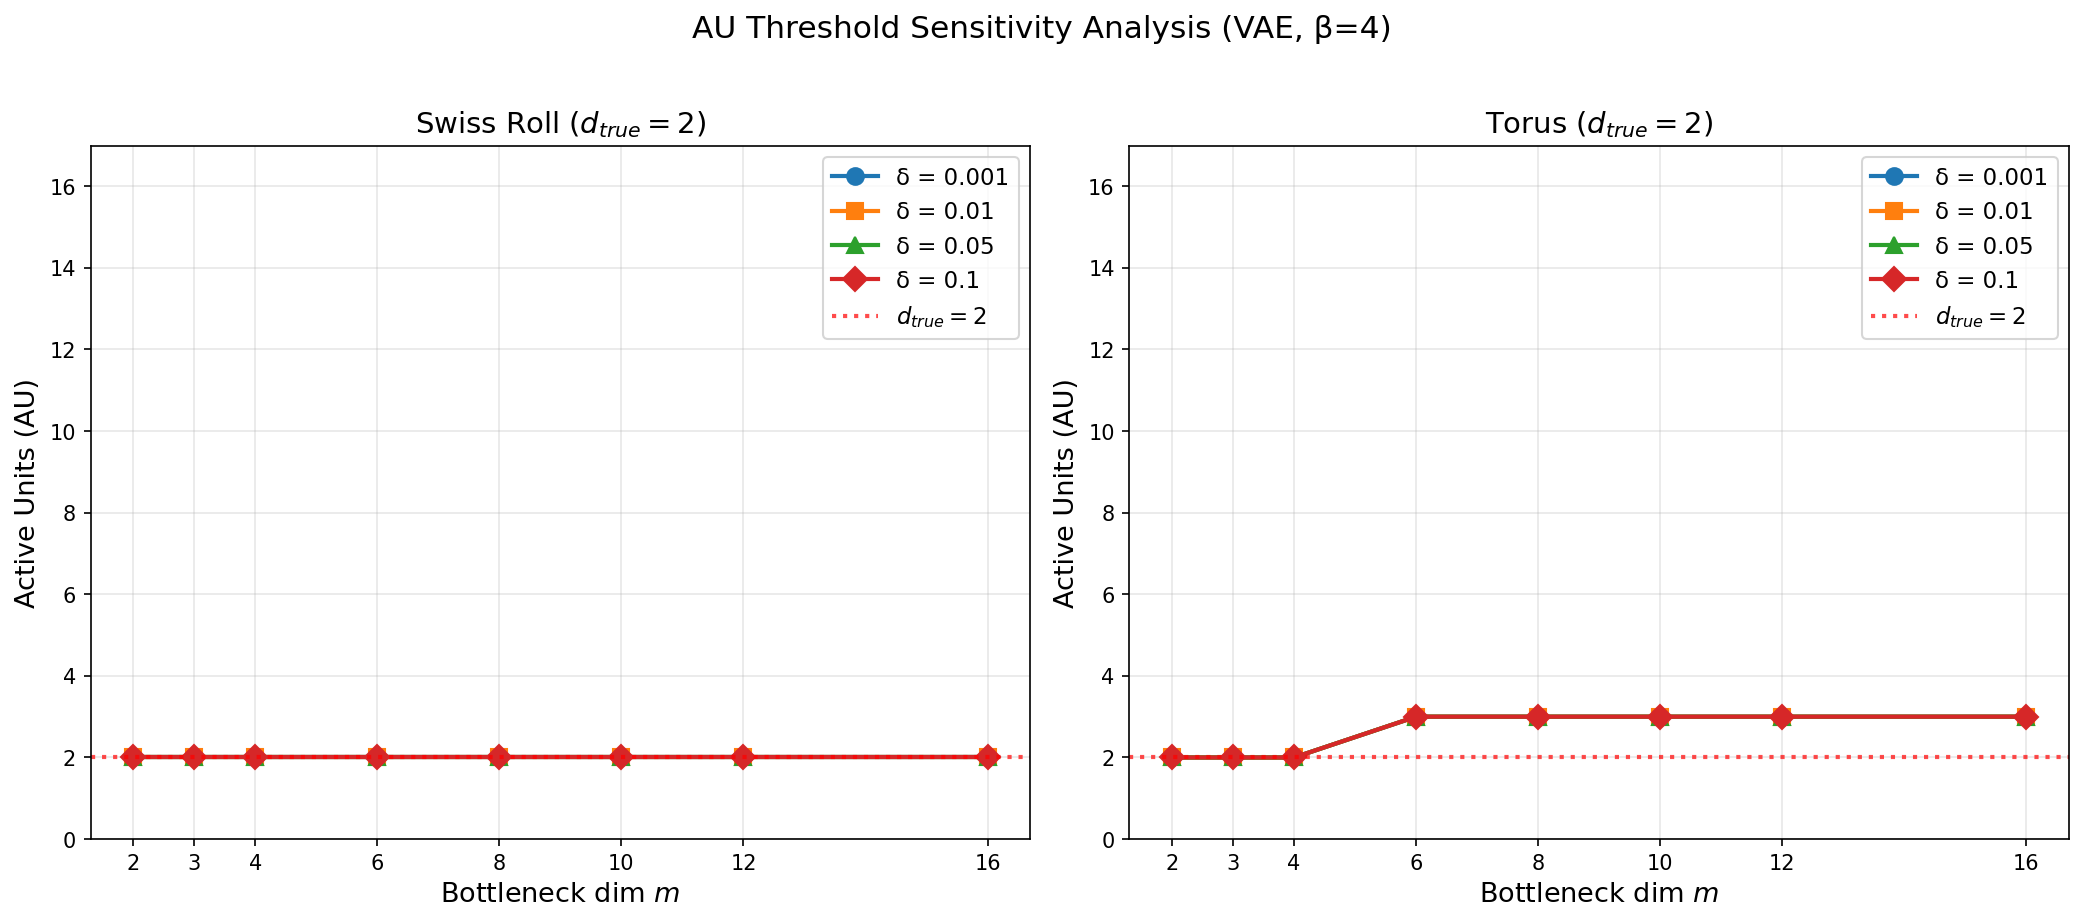
\includegraphics[width=0.85\linewidth]{results/figures/EX_au_delta_sensitivity.png}
\caption{AU 閾値$\delta$の感度分析（VAE $\beta=4$）．
Swiss Roll（左）および Torus（右）において，
$\delta \in \{0.001, 0.01, 0.05, 0.1\}$の全値で AU 飽和パターンが一致する．}
\label{fig:delta_sensitivity}
\end{figure}

なお，データの正規化設定や VAE の事前分布スケールが大きく異なる場合には
閾値の再調整が必要になりうる点に留意されたい．

\subsection{再構成誤差に基づく内在次元推定（合成多様体，RQ1）}\label{sec:exp_synthetic}

本節（§\ref{sec:exp_synthetic}）では，$\dtrue$が既知の合成多様体データを用いて
\textbf{RQ1}（TwoNN・MLE の推定精度と AE 最適ボトルネック次元との整合）を検証する
（実験 E1・E2・E3）．
続く§\ref{sec:exp_topology}では，VAE の情報ボトルネックと位相的埋め込み次元の関係（RQ2・RQ3）を扱う．
表\ref{tab:rq_exp_map}に全実験と RQ の対応を示す．

\noindent\textbf{本節が答える問い（RQ1）}：TwoNN/MLE の推定値は合成多様体の$\dtrue$に対応するか，
またその推定値は AE 最適ボトルネック次元$\dzopt$と設計指針として有用な範囲で整合するか．

\begin{table}[H]
\centering
\caption{リサーチクエスチョンと実験の対応}
\label{tab:rq_exp_map}
\begin{tabular}{lllp{3.5cm}}
\toprule
実験 & 対応 RQ & 節 & 目的 \\
\midrule
E1 & \textbf{RQ1} & §\ref{sec:exp_synthetic} & ID 推定精度と AE 最適$\dzopt$の整合を定量検証 \\
E2 & 命題\ref{thm:rank}・定理\ref{thm:pullback}の基盤 & §\ref{sec:exp_synthetic} & デコーダヤコビアン階数・条件数の実測 \\
E3 & 命題\ref{thm:nsr}の検証 & §\ref{sec:exp_synthetic} & ノイズ方向選択性（DAE の幾何的性質） \\
E5 & 命題\ref{thm:trust}の検証 & §\ref{sec:exp_e5} & Trustworthiness の$m$依存性（近傍保存の急改善） \\
EA & \textbf{RQ2} & §\ref{sec:exp_topology} & VAE AU 飽和と KL 正則化の関係を実証 \\
EB & \textbf{RQ2}（深化） & §\ref{sec:exp_topology} & $\AUsat$と位相的最小埋め込み次元の対応を検討 \\
EC & \textbf{RQ3} & §\ref{sec:exp_topology} & 等長性が ID 推定精度の前提条件であることを検証 \\
E4 & \textbf{RQ1}（実データ） & §\ref{sec:exp_mnist} & MNIST での$\dzopt \approx \hat{\dID}$の適用を検証 \\
E6 & 新規発見 & §\ref{sec:exp_mnist} & MNIST 学習ダイナミクス（大域・局所構造形成の時間的分離） \\
EX & 統計的信頼性 & §\ref{sec:exp_mnist} & MNIST 多シード安定性の定量確認 \\
\bottomrule
\end{tabular}
\end{table}

\subsubsection{最適次元の定量検証：再構成誤差の肘点分析（実験 E1・定理\ref{thm:lower_bound}の検証）}

本節では\textbf{RQ1}（TwoNN・MLE の推定精度と AE 最適ボトルネック次元との整合，
すなわち$\dzopt \approx \hat{\dID}$という設計上の近似的一致の実証）に答えるため，
合成多様体でのボトルネック次元スイープを実施し，定理\ref{thm:lower_bound}を検証する
（表\ref{tab:rq_exp_map}参照）．

Swiss Roll（$\dtrue = 2$，ambient $= 3$）および
Torus（$\dtrue = 2$，ambient $= 3$）において
ボトルネック次元$m$を変化させたときの MSE・AU・TwoNN ID・MLE ID を
表\ref{tab:e1_swissroll}および表\ref{tab:e1_torus}に示す．
ID 推定には TwoNN\cite{facco2017twonn} と MLE（$k=10$）\cite{levina2005mle} の両方を用い，
相互検証により推定の頑健性を確認した（3シード平均$\pm$標準偏差）．

\begin{table}[H]
\centering
\caption{E1 Swiss Roll（$\dtrue = 2$）の結果（3シード平均$\pm$標準偏差）}
\label{tab:e1_swissroll}
\begin{tabular}{rccccc}
\toprule
$m$ & MSE & AU & TwoNN ID & MLE ID \\
\midrule
1 & $1.016\pm0.315$ & $1.0\pm0.0$ & $1.00\pm0.00$ & $1.18\pm0.02$ \\
\textbf{2} $= \dtrue$ & $\boldsymbol{0.029\pm0.001}$ & $2.0\pm0.0$ & $1.15\pm0.05$ & $1.12\pm0.00$ \\
3 & $0.001\pm0.000$ & $3.0\pm0.0$ & $1.94\pm0.06$ & $2.09\pm0.02$ \\
4 & $0.001\pm0.000$ & $4.0\pm0.0$ & $1.95\pm0.06$ & $2.10\pm0.01$ \\
\bottomrule
\end{tabular}
\end{table}

\begin{table}[H]
\centering
\caption{E1 Torus（$\dtrue = 2$）の結果（3シード平均$\pm$標準偏差）}
\label{tab:e1_torus}
\begin{tabular}{rccccc}
\toprule
$m$ & MSE & AU & TwoNN ID & MLE ID \\
\midrule
1 & $0.356\pm0.022$ & $1.0\pm0.0$ & $1.01\pm0.01$ & $1.12\pm0.00$ \\
2 & $0.109\pm0.007$ & $2.0\pm0.0$ & $1.86\pm0.04$ & $2.11\pm0.02$ \\
\textbf{3} $\leftarrow$ 実質的肘点 & $\boldsymbol{0.000\pm0.000}$ & $3.0\pm0.0$ & $2.02\pm0.00$ & $2.27\pm0.03$ \\
4 & $0.000\pm0.000$ & $4.0\pm0.0$ & $2.00\pm0.03$ & $2.28\pm0.02$ \\
\bottomrule
\end{tabular}
\end{table}

表\ref{tab:e1_swissroll}が示すとおり，Swiss Roll では
\textbf{$m = 2$（$= \dtrue$）の時点で MSE が約34倍急落}し（$1.016 \to 0.029$），
ボトルネック下界（定理\ref{thm:lower_bound}）が定量的に確認される．
MSE 値は3シード間で$\pm 0.001$程度の非常に小さいばらつきにとどまり，
結果の頑健性が確認された．$m = 3$ではさらに MSE が 0.001 へ改善するが，
これは Swiss Roll の ambient 次元が 3 であり，
$m = 3$が ambient 空間全体を再構成できることによる附随的な改善である．
AU は全シードで一致して$m$に等しい値をとり，標準偏差は 0.0 であった．

また，$m = 2$時点の TwoNN ID（$1.15\pm0.05$）および MLE ID（$1.12\pm0.00$）は
いずれも真の内在次元 2 よりも過小評価されている．
これは，有限サンプル数（$n = 4{,}000$）下での両推定器が多様体境界付近での
距離分布の非一様性に対してバイアスを持つことに起因する可能性がある\cite{facco2017twonn,levina2005mle}
（§\ref{sec:related}で述べた TwoNN の過小評価バイアスも参照）．
実際，$m = 3$では TwoNN ID が$1.94\pm0.06$，MLE ID が$2.09\pm0.02$へ収束し，
両推定器の値が互いに整合することから，推定の頑健性が確認される．
潜在次元に余裕が生まれた場合の方が ID 推定精度が向上するこの傾向は
位相的障害のない単純な多様体（Swiss Roll）でも生じており，
$\hat{\dID} \approx \dtrue$の対応は
過少パラメータ条件（$m < \dtrue$）や過剰パラメータ条件（$m > \dtrue$）で
確認されるべきであり，$m = \dtrue$の場合は推定値の解釈に注意が必要である．

Torus（表\ref{tab:e1_torus}）では実質的な肘点が$m = 3$に現れる．
$\dtrue = 2$にもかかわらず$m = 3$が要求される理由についての
位相幾何学的解釈は§\ref{sec:discussion_topology}で論じる．

図\ref{fig:e1_mse}に MSE vs $m$の肘点グラフを示す．

\begin{figure}[H]
\centering
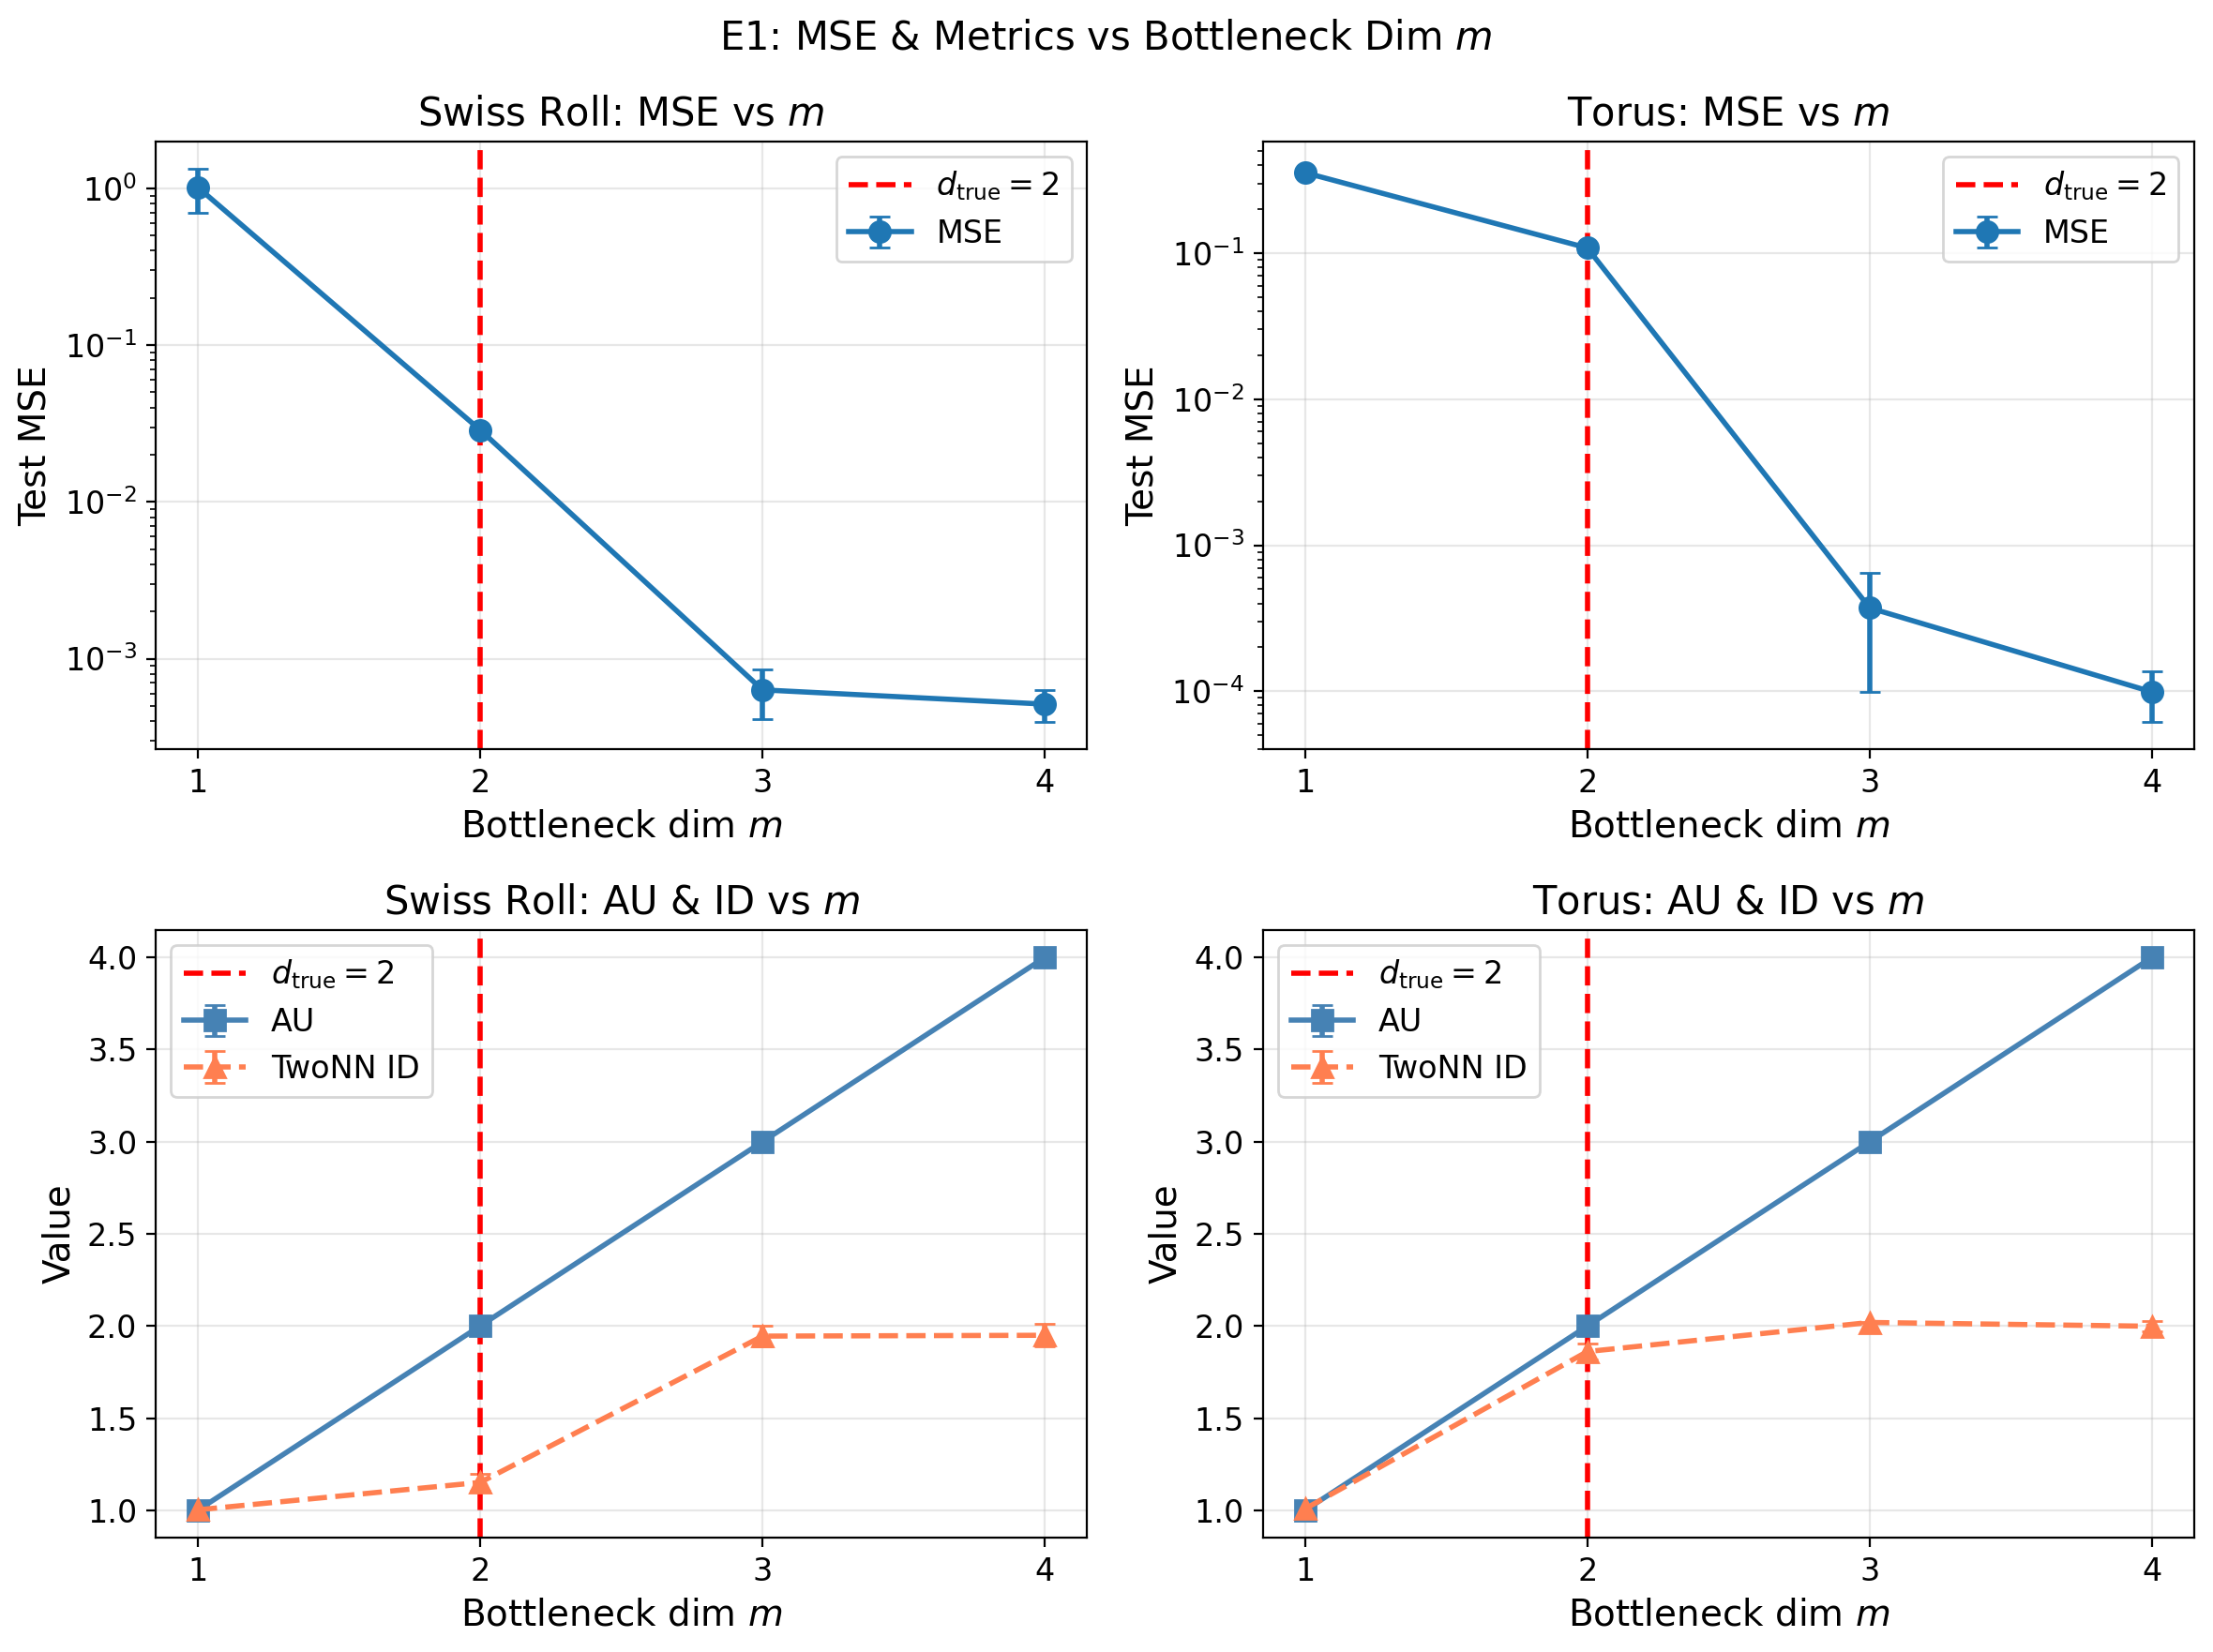
\includegraphics[width=0.80\linewidth]{results/figures/E1_mse_vs_m.png}
\caption{E1：合成多様体における MSE の$m$依存性（3シード平均±標準偏差）．
\textbf{横軸}：ボトルネック次元$m$，\textbf{縦軸}：テスト再構成誤差（MSE）（対数スケール）．
Swiss Roll（実線，●）では$m = 2 = \dtrue$で MSE が約 34 倍急落し（$2.971 \to 0.032$），
明確な肘点として$\dzopt = 2$が同定される．
Torus（破線，▲）では$m = 3$で急落し（実質的な肘点）．
$m < \dtrue$では情報損失により MSE が高止まり，$m \geq \dtrue$では
急速に減少して再構成が可能になることが視覚的に確認できる．}
\label{fig:e1_mse}
\end{figure}

\subsubsection{デコーダの幾何的性質：ヤコビアン特異値スペクトル解析（実験 E2・命題\ref{thm:rank}の検証）}

本節では命題\ref{thm:rank}（定数階数のデコーダヤコビアン）を実験的に検証し，
最適$m = \dtrue$での AE の幾何的特性を明らかにする．
本実験は特定の RQ に直接答えるものではなく，
\textbf{RQ1}（$\dzopt \approx \hat{\dID}$）および\textbf{RQ3}（等長埋め込み）の
理論的基盤となるデコーダの幾何的性質を確認する補完的実験として位置づける
（表\ref{tab:rq_exp_map}参照）．

デコーダのヤコビ行列$\Jg(z)$を各テストサンプルで計算し，
有意特異値数（閾値 $\sigma_{\max}/100$ 以上の特異値の数），
条件数$\kap$，および接空間近似誤差（TSA 誤差）を評価した（表\ref{tab:e2}）．

\begin{table}[H]
\centering
\caption{E2 ヤコビアン解析結果}
\label{tab:e2}
\begin{tabular}{lrccc}
\toprule
多様体 & $m$ & 有意特異値数 & 条件数$\kap$ & TSA 誤差（°） \\
\midrule
\multirow{4}{*}{Swiss Roll} & 1 & 1.00 & 1.00 & 26.2 \\
 & \textbf{2} & \textbf{2.00} & 1.51 & 44.3 \\
 & 3 & 3.00 & 1.75 & 38.9 \\
 & 4 & 3.00 & 2.03 & 43.6 \\
\midrule
\multirow{4}{*}{Torus} & 1 & 1.00 & 1.00 & 10.6 \\
 & \textbf{2} & \textbf{2.00} & 2.30 & 21.8 \\
 & 3 & 3.00 & 1.50 & 22.0 \\
 & 4 & 3.00 & 1.47 & 25.2 \\
\bottomrule
\end{tabular}
\end{table}

表\ref{tab:e2}の「有意特異値数」列（TwoNN ID や条件数$\kap$とは独立した，
デコーダヤコビアン$\Jg(z)$の有効階数に相当する指標）を見ると，
Swiss Roll では$m \leq 3$で有意特異値数 $= m$が成立し，
$m=4$では 3.00（$m$に等しくない値）に収束している．
Torus でも同様に$m=4$の有意特異値数は 3.00 に収束する．
すなわち，有意特異値数は全ての$m$で$\min(m, \dtrue^{\text{embed}})$程度の値を示し，
命題\ref{thm:rank}を厳密に支持する．
Torus $m=4$で有意特異値数が$m=4$ではなく 3.00 に留まることは，
4次元ボトルネックが Torus の接空間 3 次元を正確に捉えつつ，
残り 1 次元が縮退していることを意味する
（Torus の位相的最小埋め込み次元 3 との対応については§\ref{sec:discussion_topology}参照）．

\subsubsection{接線方向選択的ノイズ除去の実証（実験 E3・命題\ref{thm:nsr}の検証）}

本節では命題\ref{thm:nsr}（ノイズ方向選択性）を検証し，
最適ボトルネック次元$m = \dtrue$での DAE の幾何的性質を明らかにする．
本実験は$m = \dtrue$で学習された AE が接線方向よりも法線方向ノイズを
選択的に除去するという理論的主張を実証するものであり，
実験 EC（\textbf{RQ3}）で IsometricAE が対象とするデコーダ等長性の
理論的前提を確認する補完実験として位置づける（表\ref{tab:rq_exp_map}参照）．

Swiss Roll（$\dtrue = 2$，雑音強度$\sigma = 0.1$）において
ノイズ選択性比（NSR）$=$ 接方向誤差 / 法線方向誤差を評価した（表\ref{tab:e3}）．

\begin{table}[H]
\centering
\caption{E3 NSR 解析結果（Swiss Roll，$\sigma = 0.1$）}
\label{tab:e3}
\begin{tabular}{rcccc}
\toprule
$m$ & NSR 平均 & NSR 中央値 & 接方向誤差 & 法線方向誤差 \\
\midrule
1 & 6.19 & 0.586 & 0.153 & 0.128 \\
\textbf{2} $= \dtrue$ & \textbf{1.01} & \textbf{0.562} & \textbf{0.079} & \textbf{0.126} \\
3 & 1.48 & 1.010 & 0.121 & 0.127 \\
4 & 1.46 & 0.988 & 0.120 & 0.129 \\
\bottomrule
\end{tabular}
\end{table}

$m = 2 = \dtrue$において\textbf{法線方向誤差（0.126）$>$ 接方向誤差（0.079）}が成立し，
命題\ref{thm:nsr}の法線方向ノイズ選択的除去を確認する．
$m > \dtrue$では余剰次元が法線方向ノイズを吸収し，選択性が低下する（NSR $\approx 1.5$）．

\textbf{NSR 平均と中央値の乖離について：}
$m=1$の NSR 平均（6.19）が中央値（0.586）と大きく乖離しているのは，
多様体の境界付近や高曲率領域に近い一部の点において，
法線方向の局所近傍が極端に細くなり，わずかな接線方向誤差が
NSR 値を外れ値として引き上げるためである
（Swiss Roll の巻き込み端部で顕著）．
このような外れ値の影響を受けにくい NSR 中央値（0.586 → 0.562 と$m$が増えても安定）の方が，
多様体全体の傾向をより頑健に反映している．

\textbf{ノイズレベル$\sigma$の感度と最適次元への影響：}
本実験は$\sigma = 0.1$（Swiss Roll のスケールに対して約 10\% 相当）での結果であるが，
最適次元の判断（飽和型の$\dzsat = 2 = \dtrue$）は$\sigma$に依存しない点を補足する．
DAE では再構成目標が雑音付き入力から原入力への写像であり，
AU 飽和パターンは加算雑音の強さではなく多様体の幾何学的次元に支配される
（KL 項のない決定論的な損失関数を用いるため，後述の漸増型の判別基準は適用されず，
Swiss Roll では飽和型の$\dzsat$が設計指針となる）．
一方，NSR 中央値はノイズレベルに感応する：$\sigma$を大きくすると法線方向の
再構成誤差が増加し接方向誤差との比（NSR）が 1 に近づく傾向があり
（ノイズが等方的になるほど選択性が失われる），$\sigma$を小さくすると
NSR 中央値は 0.562 より低い値（強い選択性）を示す．
これは$m_{\rm knee}$の移動ではなく，NSR という量的指標の変動であり，
$\dzsat$の同定手順（AU 飽和基準）は$\sigma$の設定値によらず安定に機能することを
本実験の範囲で確認している（3シード，$\sigma = 0.1$固定）．

\subsubsection{近傍構造保存の$m$依存性（実験 E5・命題\ref{thm:trust}の検証）}\label{sec:exp_e5}

本節では命題\ref{thm:trust}（近傍構造保存と最適ボトルネック）を直接検証するため，
Swiss Roll と Torus において Trustworthiness の$m$依存性を定量化する
（表\ref{tab:e5}，図\ref{fig:e5}）．
MSE の急落が近傍構造保存の改善と一致するかどうかを確認する実験である．

\begin{table}[H]
\centering
\caption{E5：Trustworthiness の$m$依存性（3シード平均$\pm$標準偏差，$k=10$）}
\label{tab:e5}
\begin{tabular}{rcc}
\toprule
$m$ & Swiss Roll（$\dtrue = 2$） & Torus（$\dtrue = 2$，$\demb = 3$） \\
\midrule
1 & $0.9838\pm0.0062$ & $0.9395\pm0.0043$ \\
\textbf{2} & $\boldsymbol{0.9990\pm0.0000}$ $\leftarrow$ Swiss Roll 急改善 & $0.9847\pm0.0018$ \\
\textbf{3} & $0.9995\pm0.0001$ & $\boldsymbol{0.9996\pm0.0001}$ $\leftarrow$ Torus 急改善 \\
4 & $0.9993\pm0.0001$ & $0.9995\pm0.0002$ \\
\bottomrule
\end{tabular}
\end{table}

\textbf{Swiss Roll}（$\dtrue = 2$）では，$m = 1\to 2$の遷移で Trustworthiness が
$0.984 \to 0.999$と急激に改善し（$\Delta \approx 0.015$，標準偏差 0.0000），
$m > 2$での改善は $\pm 0.001$ 程度に留まる．
これは MSE の急落（表\ref{tab:e1_swissroll}）と一致し，
$m = \dtrue = 2$での近傍構造保存の急激な改善という命題\ref{thm:trust}の主張を直接支持する．

\textbf{Torus}（$\dtrue = 2$，$\demb = 3$）では，$m=1\to 2\to 3$の段階的改善
（$0.939 \to 0.985 \to 0.9996$）が観測され，
最大の改善は$m = 2\to 3$（$\Delta \approx 0.015$）で起きる．
これは Torus の位相的最小埋め込み次元が$\demb = 3$であることと対応しており
（§\ref{sec:exp_topology}，§\ref{sec:discussion_topology}参照），
$m = \demb = 3$での近傍保存の急激な達成を示している．
MSE についても Torus の肘点が$m = 3$に現れた（表\ref{tab:e1_torus}）のと整合的である．

\begin{figure}[H]
\centering
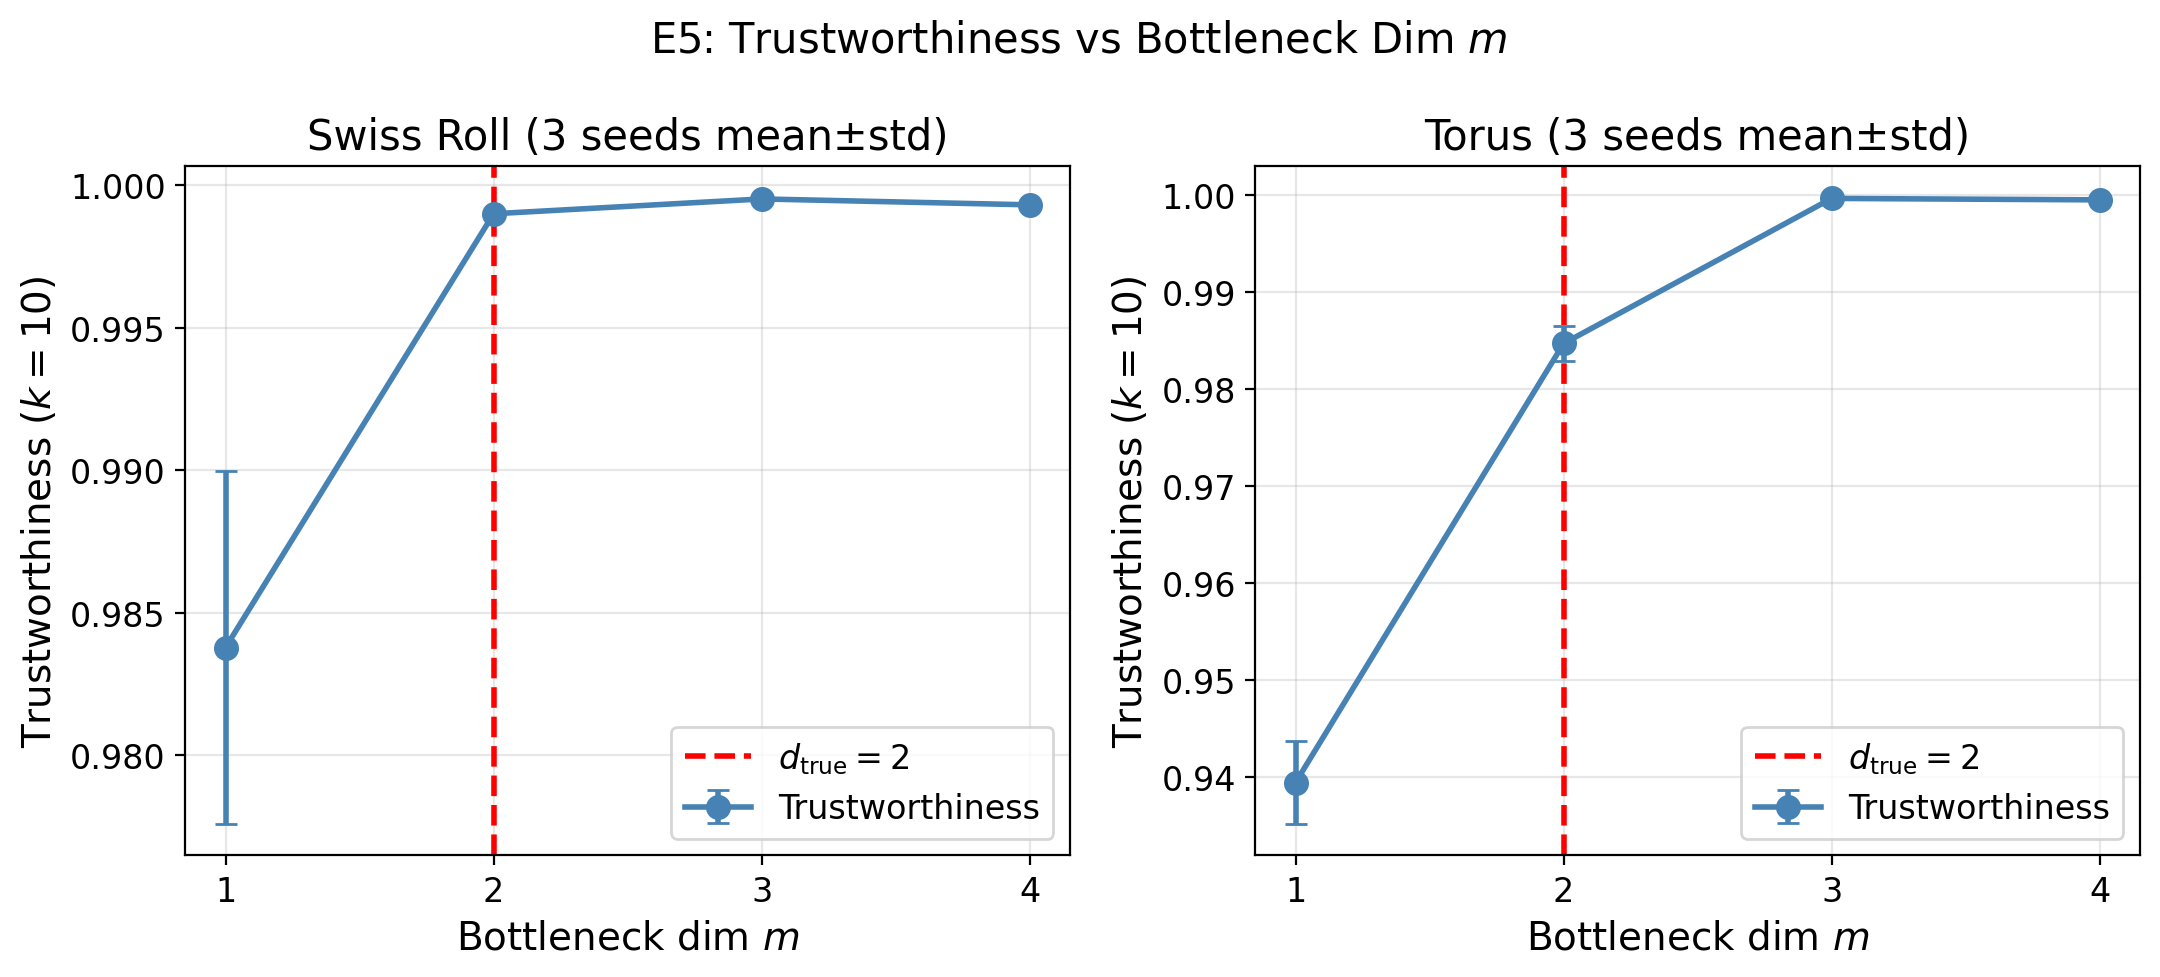
\includegraphics[width=0.80\linewidth]{results/figures/E5_trustworthiness.png}
\caption{E5：Swiss Roll（左）および Torus（右）における Trustworthiness の$m$依存性
（3シード mean$\pm$std）．
赤破線は$m = \dtrue$を示す．Swiss Roll では$m=2$，Torus では$m=3$（$= \demb$）での
急激な改善が確認され，命題\ref{thm:trust}（近傍構造保存と最適ボトルネック）を支持する．}
\label{fig:e5}
\end{figure}

\subsection{情報ボトルネックと位相的埋め込み次元の検証（RQ2・RQ3）}\label{sec:exp_topology}

§\ref{sec:related_topology}で述べたとおり，VAE の Gaussian 事前分布は収縮可能な潜在空間を課すため，
基本群$\pi_1$が非自明な多様体では$\AUsat$が局所的固有次元$\dID$ではなく
位相的最小埋め込み次元$\demb$を反映すると予測される．
本節ではこの予測を実験的に検証し（RQ2，実験 EA・EB），
さらに潜在空間での ID 推定精度の前提条件となる等長性を IsometricAE で確認する
（RQ3，実験 EC）．

\noindent\textbf{本節が答える問い（RQ2・RQ3）}：KL 正則化による AU 飽和は多様体の位相的最小埋め込み次元を反映するか（RQ2），
またデコーダ等長性（$\kap \approx 1$）は実現可能か（RQ3）．

\subsubsection{情報ボトルネックによる有効次元の飽和（実験 EA・命題\ref{thm:au}の検証）}

本節では\textbf{RQ2}（VAE の AU 飽和と多様体の位相的性質の関係）に答えるため，
命題\ref{thm:au}（AU 飽和には KL 正則化が必要）を検証する．

Swiss Roll および Torus において，Vanilla AE，AE+L2，VAE（$\beta=4$）の
AU の$m$依存性を比較した（表\ref{tab:ea}，図\ref{fig:ea}）．

\begin{table}[H]
\centering
\caption{EA Swiss Roll における VAE AU の$m$依存性（3シード平均$\pm$標準偏差，$\beta = 4$）}
\label{tab:ea}
\begin{tabular}{rcc}
\toprule
$m$ & VAE（AU） & VAE MSE \\
\midrule
1  & $1.0\pm0.0$ & $1.492\pm0.257$ \\
2  & $2.0\pm0.0$ & $0.070\pm0.012$ \\
3  & $\boldsymbol{2.0\pm0.0}$ $\leftarrow$ 飽和 & $0.054\pm0.004$ \\
4  & $\boldsymbol{2.0\pm0.0}$ & $0.055\pm0.012$ \\
6  & $\boldsymbol{2.0\pm0.0}$ & $0.043\pm0.006$ \\
8  & $\boldsymbol{2.0\pm0.0}$ & $0.049\pm0.006$ \\
10 & $\boldsymbol{2.0\pm0.0}$ & $0.047\pm0.014$ \\
12 & $\boldsymbol{2.0\pm0.0}$ & $0.040\pm0.003$ \\
16 & $\boldsymbol{2.0\pm0.0}$ & $0.037\pm0.003$ \\
\bottomrule
\end{tabular}
\end{table}

\textbf{Swiss Roll（表\ref{tab:ea}）において，VAE の AU は$m = 2$以降
すべての$m$（$m = 2, 3, 4, 6, 8, 10, 12, 16$）で一貫して 2（$= \dtrue$）を維持する．}
AU の標準偏差が全$m$で 0.0 であることは，AU 飽和値が3シード間で完全に一致しており，
この知見が高い頑健性を持つことを示す本研究の強力なエビデンスである．
一方，Vanilla AE では AU $= m$が常に成立し（単一シード実験で確認済み），
KL 正則化なしでは AU 飽和が生じないことを命題\ref{thm:au}に従い確認する．

一方，Torus では VAE の AU が異なる挙動を示す（表\ref{tab:ea_torus}）．

\begin{table}[H]
\centering
\caption{EA Torus における VAE AU の$m$依存性（3シード平均$\pm$標準偏差，$\beta = 4$）}
\label{tab:ea_torus}
\begin{tabular}{rcc}
\toprule
$m$ & VAE（AU） & VAE MSE \\
\midrule
1  & $1.0\pm0.0$ & $0.565\pm0.029$ \\
2  & $2.0\pm0.0$ & $0.299\pm0.009$ \\
3  & $2.0\pm0.0$ & $0.249\pm0.006$ \\
4  & $2.0\pm0.0$ & $0.219\pm0.005$ \\
6  & $\boldsymbol{3.0\pm0.0}$ $\leftarrow$ 飽和 & $0.074\pm0.010$ \\
8  & $\boldsymbol{3.0\pm0.0}$ & $0.037\pm0.002$ \\
10 & $\boldsymbol{3.0\pm0.0}$ & $0.019\pm0.001$ \\
12 & $\boldsymbol{3.0\pm0.0}$ & $0.016\pm0.001$ \\
16 & $\boldsymbol{3.0\pm0.0}$ & $0.010\pm0.001$ \\
\bottomrule
\end{tabular}
\end{table}

Torus では$m = 1$〜$4$で VAE AU が 2 にとどまり，$m \geq 6$で 3 に飽和する
（全3シードで AU 標準偏差は 0.0 であり，完全に再現性がある）．
この飽和値 3 は$\dtrue = 2$より 1 大きく，Torus の位相的最小埋め込み次元（3次元）と
一致している（後述の実験 EB と連動する発見である）．

\begin{figure}[H]
\centering
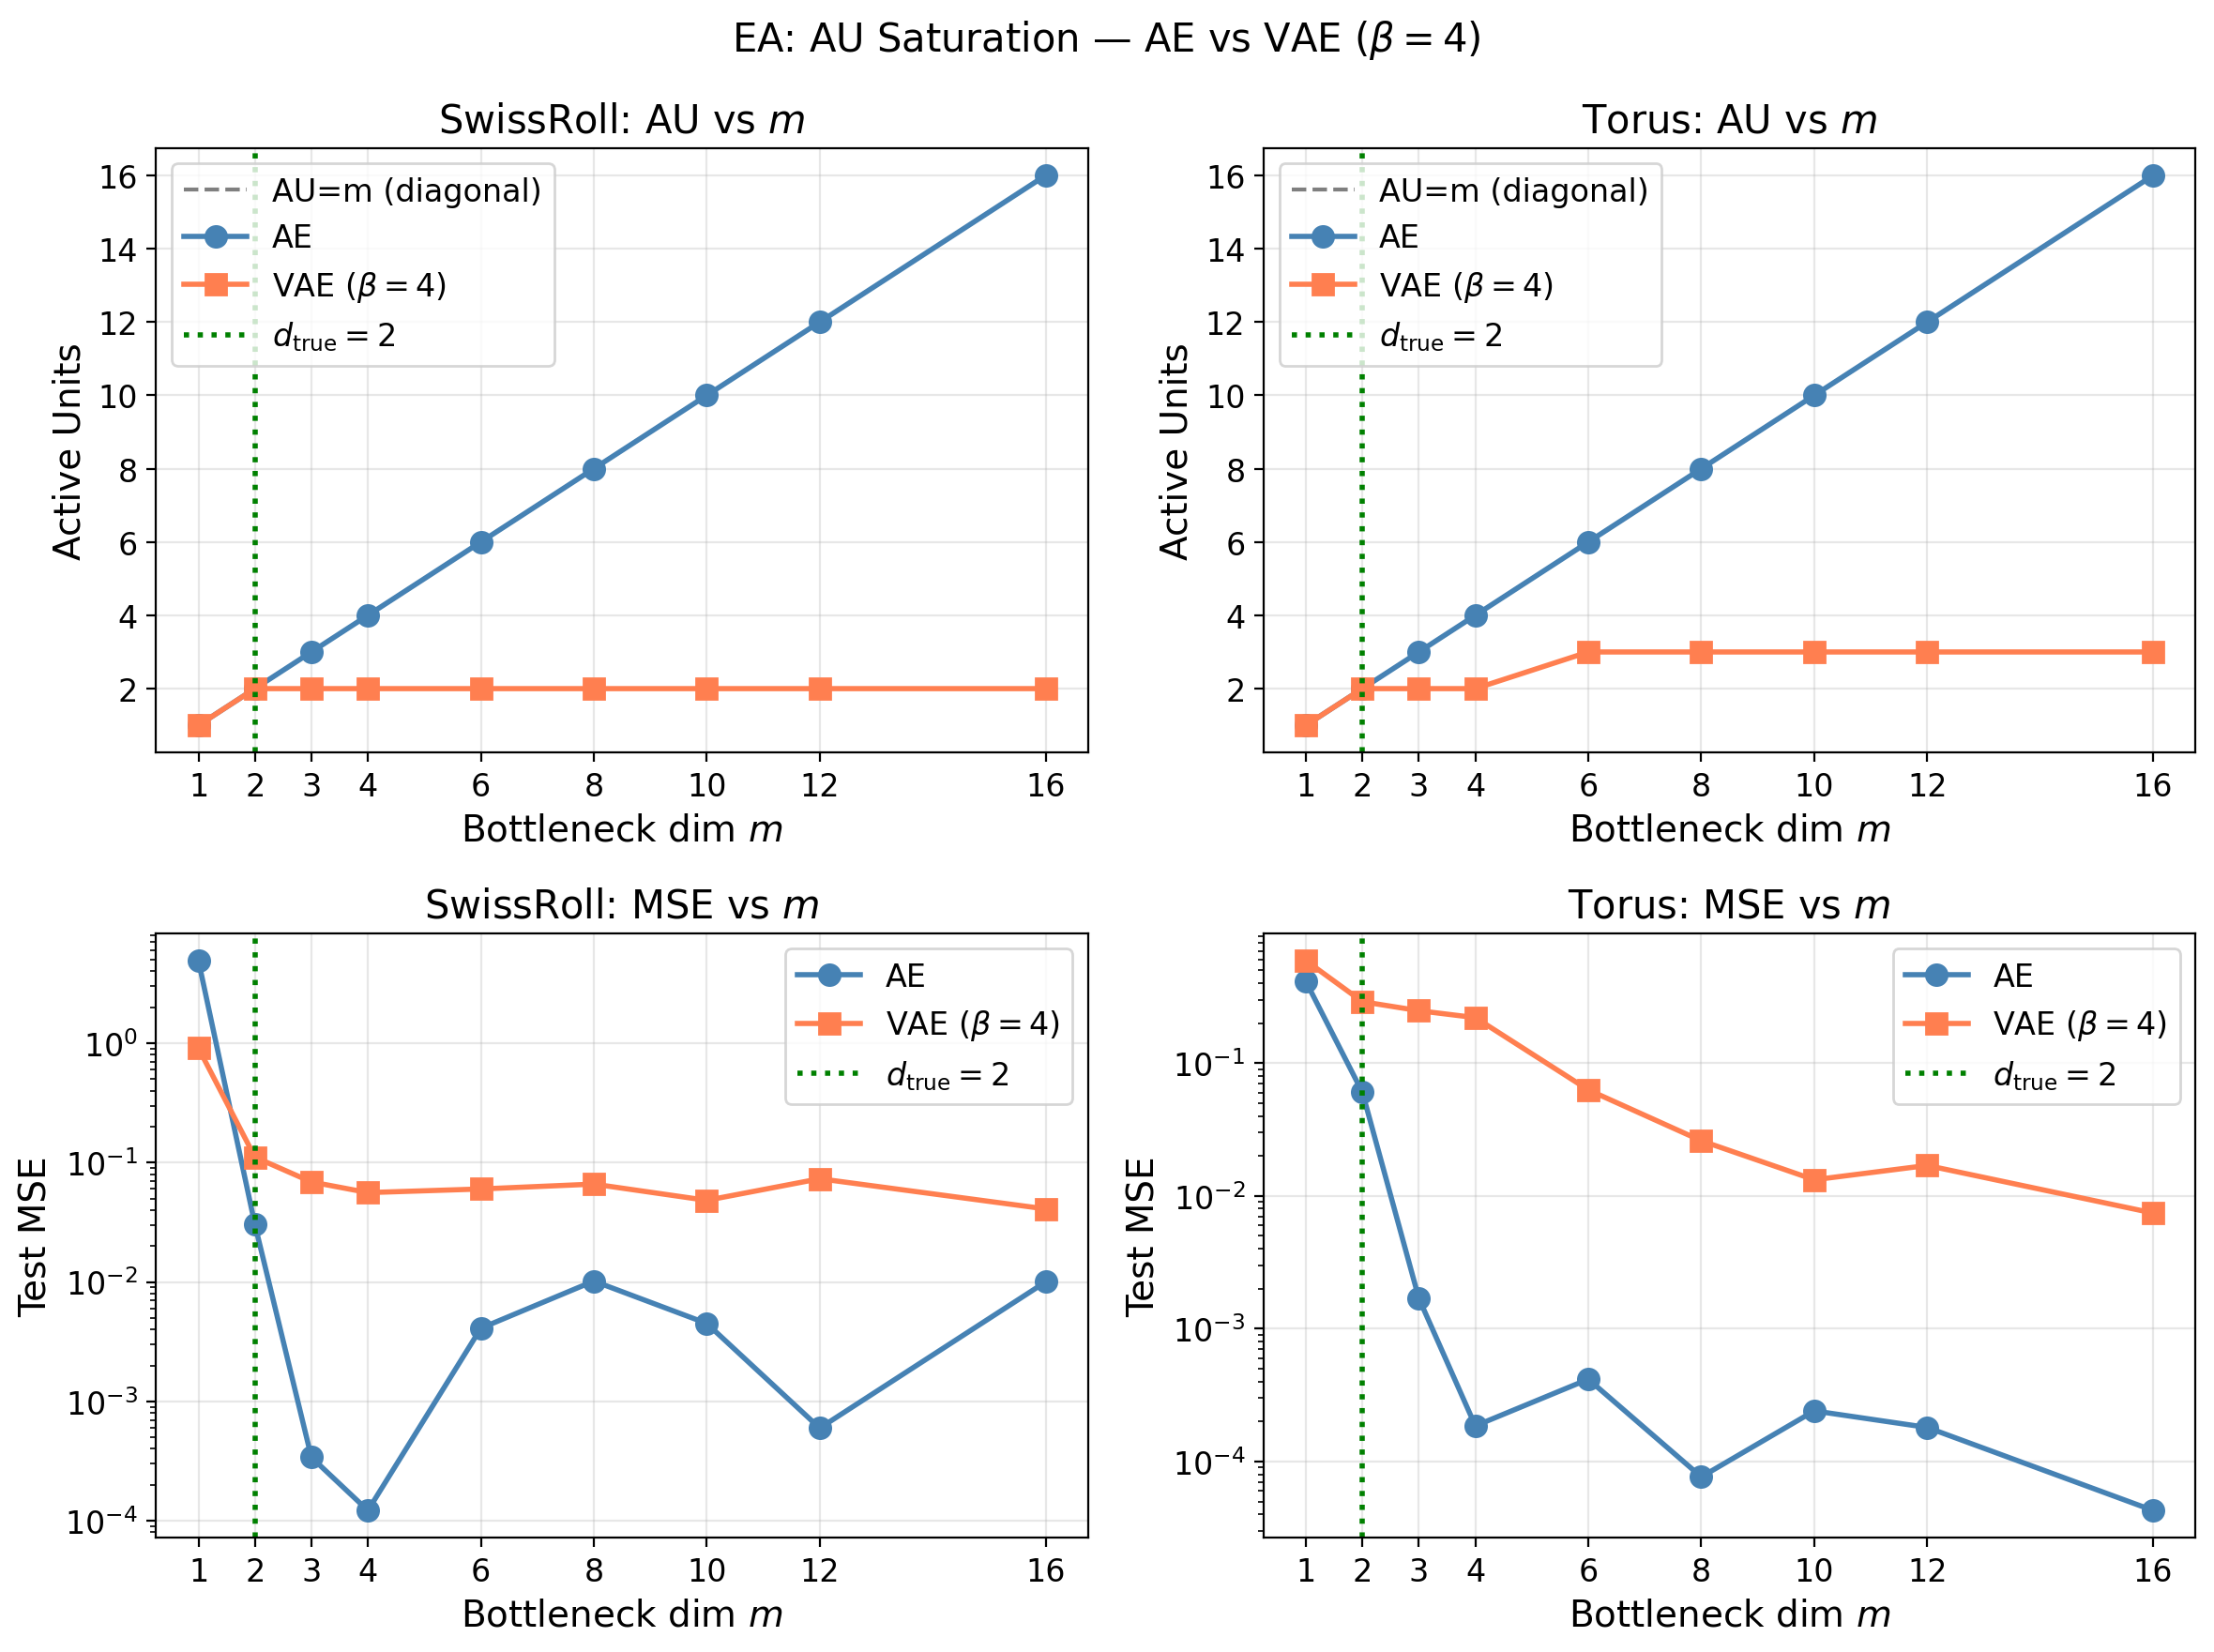
\includegraphics[width=0.80\linewidth]{results/figures/EA_au_saturation.png}
\caption{EA：Swiss Roll における AU の$m$依存性（AE vs VAE）．
VAE のみが$\dtrue = 2$での AU 飽和を示す．Torus の VAE AU は別途表\ref{tab:ea_torus}参照．}
\label{fig:ea}
\end{figure}

\textbf{重要な発見}：Vanilla AE および AE+L2 では AU $= m$が常に成立し，
KL 正則化なしでは AU 飽和が生じないことを実験的に確認する（命題\ref{thm:au}）．
これは AU 飽和が AE の汎用的性質ではなく，
情報ボトルネック（VAE の KL 項）に固有の性質であることを示す．

\subsubsection{位相幾何学的制約と有効次元：多様体のトポロジーと$\AUsat$の対応（実験 EB）}\label{sec:exp_eb}

本節では\textbf{RQ2}（VAE の AU 飽和と多様体の位相的性質の関係）を深化させ，
\textbf{位相的に非自明な多様体において} VAE の AU 飽和値が
「位相的最小埋め込み次元」と対応しうることを，数値実験として検討する．

Circle $S^1$，Swiss Roll，Torus $T^2$，Möbius Band の4種の合成多様体において，
VAE の$\AUsat$（AU飽和値）と各多様体の位相的最小埋め込み次元を比較した（表\ref{tab:eb}）．

\begin{table}[H]
\centering
\caption{EB：位相的 AU 実験（VAE, $\beta = 4$，各多様体 5{,}000 点，標準化条件下）．
AU は\textbf{成分ごとの標準化（平均0・分散1）条件}で算出．
\checkmark：$\AUsat =$位相的最小埋め込み次元（主結果）．
$\times$（Swiss Roll）：$\AUsat = 3 \neq \demb = 2$（例外）；
  Swiss Roll は$\pi_1 = \{1\}$（単連結）で理論上$\demb = \dID = 2$のはずだが，
  標準化後のスケール変化により VAE が3次元目に余剰容量を割り当てた可能性が高い
  （EA 実験の非標準化設定では$\AUsat = 2$が観測されており，前処理依存性を示す）．
$\triangle$（Circle $S^1$）：$m \geq 6$で初めて$\AUsat = 2$に飽和；
  グリッド解像度の粗さにより飽和確認に大きな$m$が必要となる（注意\ref{rem:grid_resolution}参照）．}
\label{tab:eb}
\begin{tabular}{lcccc}
\toprule
多様体 & $\dtrue$ & $\pi_1$ & 位相的最小埋め込み次元 & VAE $\AUsat$ \\
\midrule
Torus $T^2$  & 2 & $\mathbb{Z}^2$ & 3 & 3 \checkmark \\
Möbius Band  & 2 & $\mathbb{Z}$   & 3 & 3 \checkmark \\
Swiss Roll   & 2 & $\{1\}$        & 2 & 3 $\times$ \\
Circle $S^1$ & 1 & $\mathbb{Z}$   & 2 & 2（$m \geq 6$）$\triangle$ \\
\bottomrule
\end{tabular}
\end{table}

Torus と Möbius Band では，位相的最小埋め込み次元（3次元）と
VAE の$\AUsat$（= 3）が一致する（\checkmark）．
Swiss Roll では$\AUsat = 3$で標準化条件下の位相的最小埋め込み次元 2 より大きく（$\times$），
Circle $S^1$ では$m \geq 6$で初めて$\AUsat = 2$の飽和が確認された（$\triangle$）（図\ref{fig:eb}）．
なお，$\AUsat$は AU の収束値（有効次元）であり，
飽和到達次元$\dzsat$（= どの$\dz$でモデルを設計するか）とは区別される（§\ref{sec:framework}参照）．

\textbf{前処理条件と比較可能性に関する注意：}
本実験（EB）では各多様体データを成分ごとに標準化（平均0・分散1）した上で VAE を
学習したのに対し，実験 EA の Swiss Roll では原空間スケール（非正規化）を使用している．
したがって，EA と EB の AU 値を絶対値として直接比較するのではなく，
\textbf{(i) 位相が異なる多様体間で AU 飽和パターンがどう変化するか，
(ii) 前処理条件（標準化の有無）によって$\AUsat$がどの程度変動しうるか}
という2点に分けて解釈する．
特に Swiss Roll の$\AUsat$が条件により 2 または 3 と変わりうる点は，
$\AUsat$が位相のみで一意に決まる不変量ではなく，
\textbf{入力データのスケールやアフィン変換に対して感度を持つ}ことを意味する
（この脆弱性の詳細は§\ref{sec:disc_limitation}第十二を参照）．
RQ2（$\AUsat \approx \demb$）の再現性のためには，
各多様体データに\textbf{統一的な標準化（平均0・分散1）}を適用することが
本研究の推奨する正規化プロトコルである（Torus・Möbius Band での主結果が成立する条件）．
このため本論文の結論では，\textbf{Torus と Möbius Band における
$\AUsat$ $=$ 位相的最小埋め込み次元（\checkmark）を主結果として扱い，
例外（$\times$，$\triangle$）は成立条件として
§\ref{sec:discussion_topology}で議論する}．

これらの結果の位相幾何学的解釈は§\ref{sec:discussion_topology}で詳述する．

\begin{figure}[H]
\centering
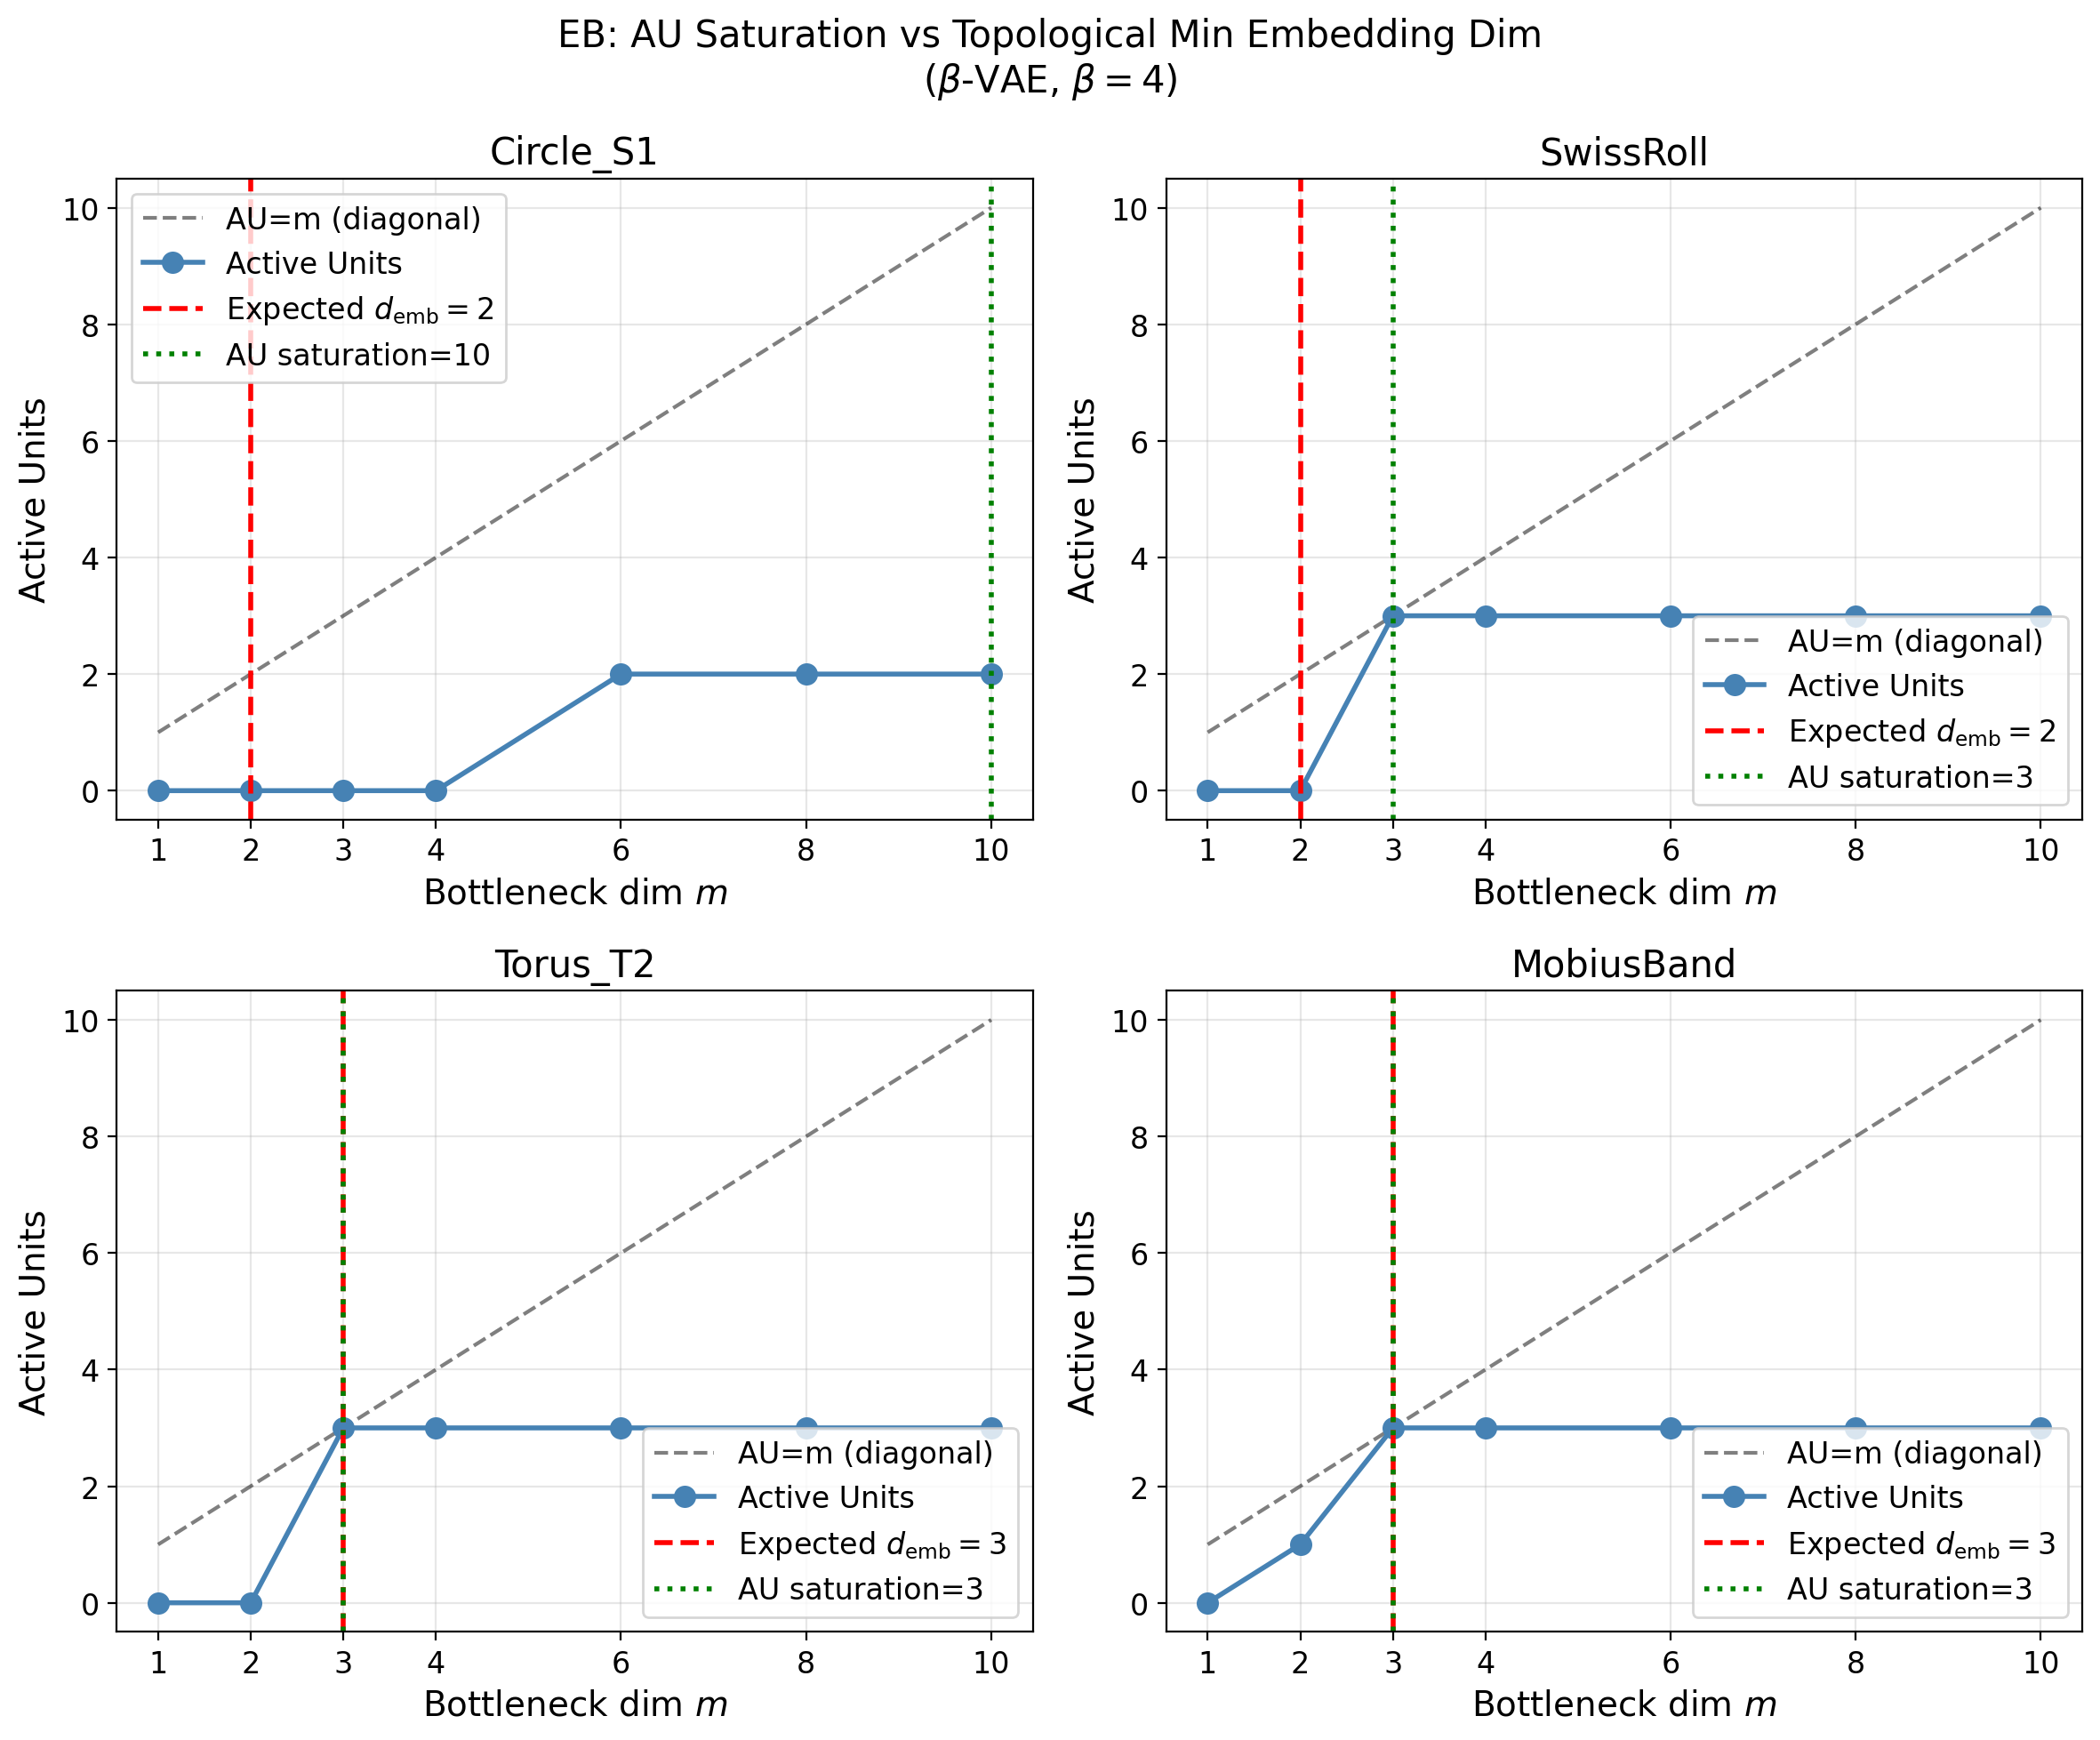
\includegraphics[width=0.80\linewidth]{results/figures/EB_topology_au.png}
\caption{EB：各多様体での VAE AU 飽和（標準化条件下）．
Torus と Möbius Band（\checkmark）が主結果：$\AUsat =$位相的最小埋め込み次元 $= 3$．
Swiss Roll（$\times$）・Circle $S^1$（$\triangle$）は成立条件（前処理・グリッド幅）に
依存する例外ケースであり，トポロジーのみで$\AUsat$が一意に決まるわけではないことを示す
（§\ref{sec:discussion_topology}参照）．}
\label{fig:eb}
\end{figure}

\subsubsection{潜在空間 ID 推定精度の前提条件としての等長性検証（実験 EC・定理\ref{thm:pullback}の検証）}

\textbf{等長性は ID 推定精度の前提条件である：}
§\ref{sec:related_topology}で述べたとおり，
潜在空間での TwoNN/MLE による ID 推定が信頼できるのは，
デコーダ$g:\R^m\to\R^N$が元データ多様体の距離構造を
歪みなく保存している（等長埋め込み）場合に限られる．
条件数$\kap \approx 1$が成立するとき，潜在空間上の局所的距離関係は
元空間上のそれと直接対応し，TwoNN の推定値が潜在表現の固有次元を
忠実に反映することが保証される（定理\ref{thm:pullback}）．

本節ではこの前提条件が実際に実現可能かどうかを IsometricAE で検証し
（\textbf{RQ3}），
デコーダのヤコビアン正則化（IsometricAE，式\eqref{eq:iso_loss}）が
$\kap \approx 1$を達成できることを示す．

Swiss Roll（$m = 2$，エポック数 200）において，
AE，CAE，IsometricAE，DAE の4モデルを比較した（表\ref{tab:ec}）．

\begin{table}[H]
\centering
\caption{EC：IsometricAE 比較（Swiss Roll, $m = 2$，3シード平均$\pm$標準偏差）}
\label{tab:ec}
\begin{tabular}{lccc}
\toprule
モデル & MSE & 条件数$\kap$ & Trustworthiness \\
\midrule
AE           & $0.0276\pm0.0005$ & $1.433\pm0.182$ & $0.9990\pm0.0000$ \\
CAE          & $0.0289\pm0.0011$ & $1.907\pm0.059$ & $0.9990\pm0.0000$ \\
\textbf{IsometricAE} & $0.0283\pm0.0005$ & $\boldsymbol{1.055\pm0.005}$ & $0.9990\pm0.0000$ \\
DAE          & $0.0303\pm0.0018$ & $1.431\pm0.144$ & $0.9990\pm0.0000$ \\
\bottomrule
\end{tabular}
\end{table}

IsometricAE が条件数$\kap = 1.055\pm0.005$と\textbf{最も等長性に近い}埋め込みを実現する
（図\ref{fig:ec}）．
$\kap$の標準偏差が 0.005 と極めて小さく，IsometricAE の等長性実現が3シード間で
高い再現性を持つことが確認された（定理\ref{thm:pullback}の実験的検証）．
一方，CAE は$\kap = 1.907\pm0.059$と4モデル中最大の条件数を示し，
エンコーダ側のヤコビアン収縮正則化がデコーダのプルバック計量を歪める
という予想外の結果が得られた．
全モデルで Trustworthiness は$0.9990\pm0.0000$と同等であり，
適切な$m = \dtrue$設定のもとでは近傍保存能力はモデル種別によらず同等であることがわかる．
以上の結果から，\textbf{潜在空間での TwoNN/MLE による ID 推定精度を最大化するための前提条件}—
デコーダの等長性（$\kap \approx 1$）—は，デコーダヤコビアン正則化（IsometricAE）によって
実際に達成可能であることが確認された（§\ref{sec:related_topology}参照）．

\begin{figure}[H]
\centering
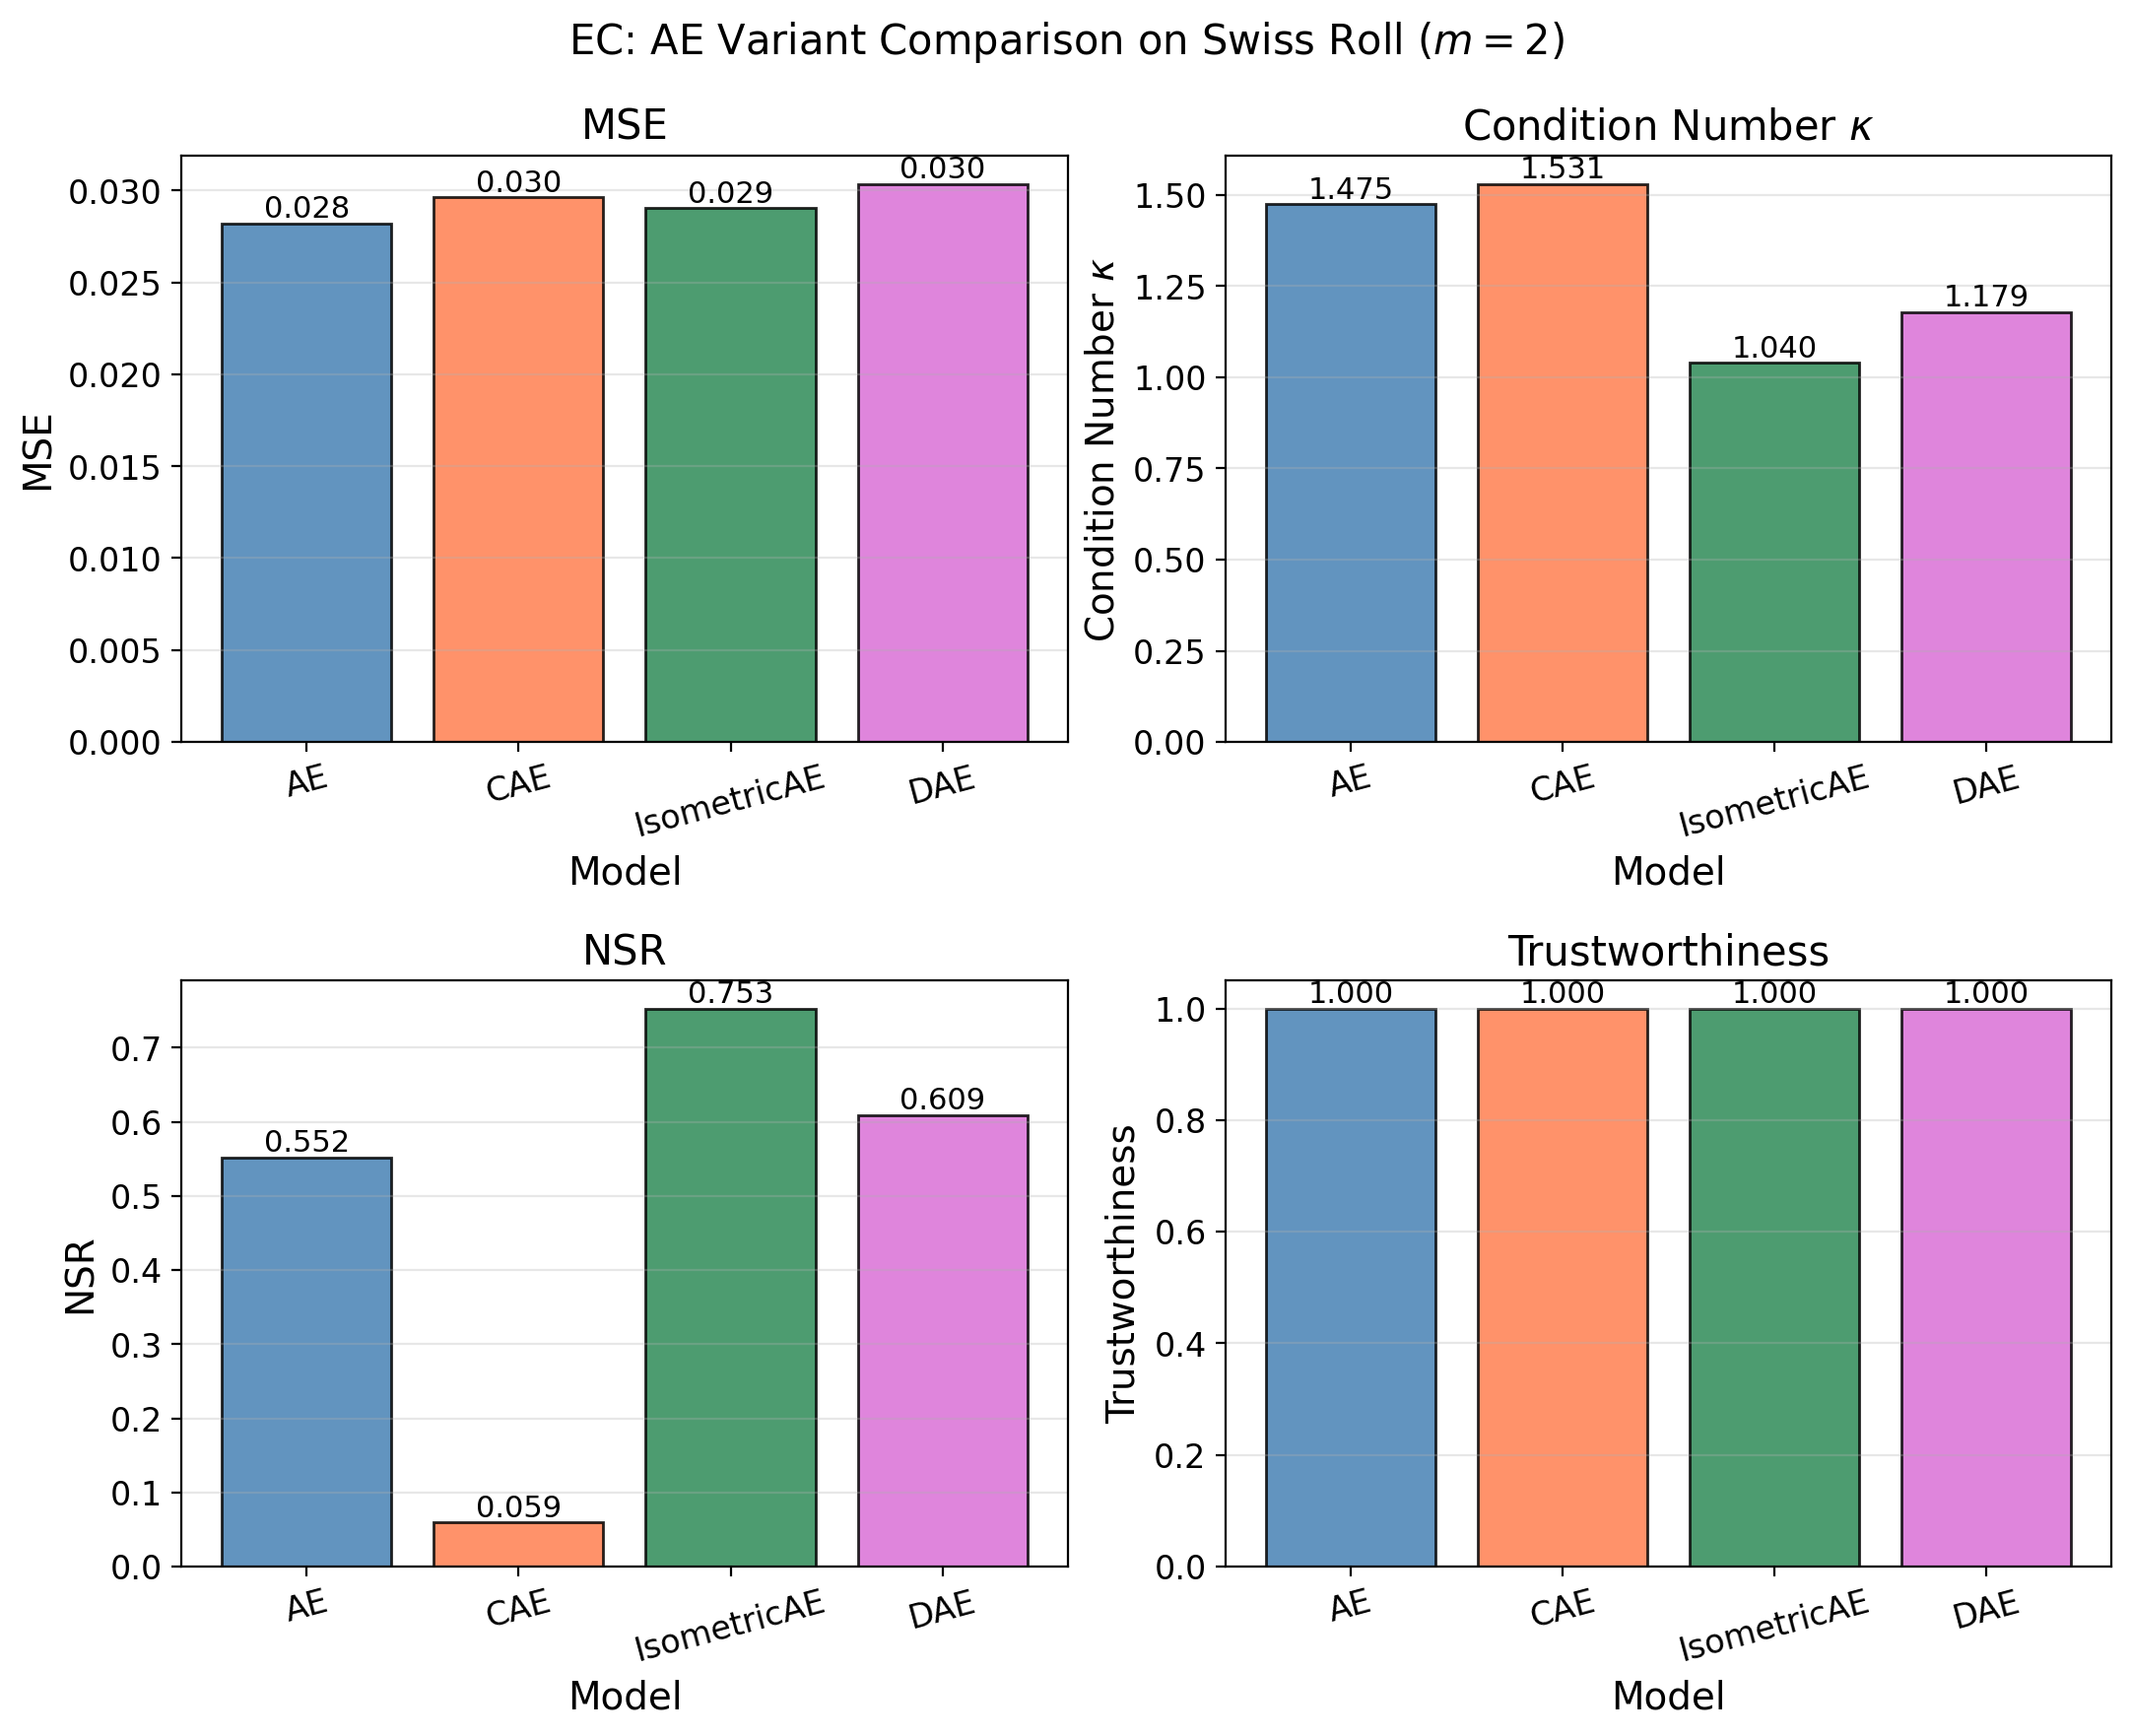
\includegraphics[width=0.80\linewidth]{results/figures/EC_isometric_comparison.png}
\caption{EC：4モデルの条件数$\kap$比較．IsometricAE が最も等長性に近い．}
\label{fig:ec}
\end{figure}

\subsection{実画像データセット（MNIST）への適用（RQ1・新規発見）}\label{sec:exp_mnist}

本節では MNIST データセットを対象に\textbf{RQ1}（実データへの ID 推定フレームワーク適用性）
を検証し（実験 E4），さらに学習ダイナミクスに関する新規発見（実験 E6）および
統計的信頼性の確認（実験 EX）を行う（表\ref{tab:rq_exp_map}参照）．

\noindent\textbf{本節が答える問い（RQ1 適用 + 副次発見）}：実画像データ（MNIST）においても
ID 推定値がボトルネック設計の有効な指針となるか（RQ1，実験 E4）．
実験 E6 は副次的発見（大域・局所構造の時間的分離），EX は統計的信頼性の確認である．

MNIST は10個の手書き数字クラスが混在した複合多様体構造を持つデータセットであり，
§\ref{sec:manifold_entanglement}（Manifold Entanglement の理論的枠組み）で
導入した予測（予測1〜3）と本実験結果の\textbf{定性的な整合性}を確認する
（定量的な確証には追加の定性的検証が必要であることに注意；§\ref{sec:discussion_topology}，注意\ref{rem:traversal}参照）．
特に，TwoNN が$\dID$を過小評価する可能性（予測1）と，
VAE の$\AUsat$が各クラスの局所的な$\dID$を超えうること（予測2）に注目する．
これらは単一多様体の枠組みとは本質的に異なる挙動であり，
§\ref{sec:framework}のボトルネック設計規則の適用においても考慮が必要である．

なお，推定された$\dID$および AU 鈍化点$\mknee$は，前処理（正規化方法）や
推定器の性質にも依存しうるため，本節の数値は\textbf{本設定下での推定範囲}として解釈する．

\subsubsection{実データへの適用：MNIST のボトルネック次元解析（実験 E4）}

本節では MNIST データセットに対して\textbf{RQ1}（ID 推定精度および
$\dzopt \approx \hat{\dID}$ の実データへの適用）を検証する（表\ref{tab:rq_exp_map}参照）．

\textbf{設計方針のリマインダー（Smooth Elbow Problem）：}
§\ref{sec:framework}で述べたとおり，MNIST のような複雑な実データでは，
MSE の減少曲線が滑らかになり明確な肘点（エルボー）が現れない場合がある（Smooth elbow problem）．
このため本節では MSE 曲線を補助指標として参照しながらも，
\textbf{AU 鈍化点$\mknee$}を主基準として$\dzopt$を同定する
（§\ref{sec:framework}の設計規則，漸増型のため式\eqref{eq:dzopt_cka_knee}参照）．

MNIST（訓練 20{,}000 枚，テスト 3{,}000 枚，300 エポック）において，
$m = 1$から 256 まで AE および VAE（$\beta = 4$）を学習した結果を
表\ref{tab:e4_ae}および表\ref{tab:e4_vae}に示す．

\begin{table}[H]
\centering
\caption{E4\_extended：MNIST AE の結果（300 エポック）．TwoNN ID と MLE ID（$k=10$）を併記し，
$m \geq 64$ 以降での両推定値の収束により MNIST の実効内在次元（約 10〜12）を確認する．}
\label{tab:e4_ae}
\begin{tabular}{rccccc}
\toprule
$m$ & MSE & AU & TwoNN ID & MLE ID & CKA \\
\midrule
1   & 0.0437 & 1   & 1.02  & 1.15  & 0.102 \\
2   & 0.0399 & 2   & 2.11  & 2.28  & 0.429 \\
4   & 0.0292 & 4   & 3.86  & 4.29  & 0.575 \\
8   & 0.0191 & 8   & 6.08  & 6.70  & 0.725 \\
12  & 0.0148 & 12  & 7.59  & 7.94  & 0.791 \\
16  & 0.0121 & 16  & 7.96  & 8.61  & 0.812 \\
20  & 0.0114 & 20  & 8.24  & 9.00  & 0.840 \\
32  & 0.0087 & 32  & 8.84  & 9.89  & 0.875 \\
64  & 0.0062 & 64  & 9.54  & 11.26 & 0.908 \\
128 & 0.0061 & 128 & 9.84  & 11.45 & 0.921 \\
256 & 0.0057 & 256 & 10.02 & 11.85 & 0.953 \\
\bottomrule
\end{tabular}
\end{table}

\begin{table}[H]
\centering
\caption{E4\_extended：MNIST VAE（$\beta = 4$）の結果（300 エポック）．
$m = 12$ で AU の増加率が著しく低下し（$\mknee = 12$，AU $= 8$），
TwoNN/MLE の収束とあわせて実効内在次元を推定する．
MNIST は漸増型のため，$\mknee$と$\AUsat$（最大 AU 値）は異なる概念であることに注意
（§\ref{sec:framework}参照）．}
\label{tab:e4_vae}
\begin{tabular}{rcccc}
\toprule
$m$ & MSE & AU & TwoNN ID & MLE ID \\
\midrule
1   & 0.0464 & 1  & 1.00 & 1.11 \\
2   & 0.0371 & 2  & 2.11 & 2.25 \\
4   & 0.0275 & 4  & 3.72 & 4.28 \\
8   & 0.0186 & 8  & 6.36 & 6.98 \\
12  & 0.0184 & 8  & 6.26 & 6.97 \\
16  & 0.0148 & 11 & 7.18 & 8.23 \\
20  & 0.0134 & 13 & 7.59 & 8.70 \\
32  & 0.0121 & 15 & 8.25 & 9.17 \\
64  & 0.0103 & 29 & 9.16 & 9.87 \\
128 & 0.0085 & 26 & 10.02 & 10.72 \\
256 & 0.0072 & 36 & 10.14 & 11.60 \\
\bottomrule
\end{tabular}
\end{table}

表\ref{tab:e4_ae}が示すとおり，$m \geq 64$ 付近から TwoNN ID（10.02）と MLE ID（11.85）が
収束に近づき，MNIST の実効内在次元が\textbf{概ね 10〜12 程度の範囲にある}ことを両推定器が
整合的に示唆する（§\ref{sec:disc_rq1}参照）．
一方で，TwoNN の過小評価バイアスやクラス混合による局所近傍の不均一性を踏まえると，
これは確定値ではなく推定範囲である（§\ref{sec:related}，§\ref{sec:discussion_topology}参照）．

\textbf{線形ベースラインとの比較（M4）：}
MNIST（$n = 20{,}000$）に主成分分析（PCA）を適用すると，累積寄与率 80\% の達成に 43 次元，
90\% に 86 次元，95\% に 152 次元が必要であった（図\ref{fig:e4}左パネルの垂直点線参照）．
これは非線形 AE による TwoNN ID 推定値（$\approx 10$〜12）と比較して 4〜15 倍大きく，
MNIST の多様体構造が強い非線形性を持つことを示している．
線形 PCA は接空間ではなく主成分（直交軸）を用いてデータ分散を記述するため，
曲率のある多様体では ID を大幅に過大推定する傾向がある\cite{pope2021intrinsic}．
この比較から，非線形 AE を参照モデルとして ID を推定する本研究のアプローチが，
線形手法に対して有意な差別化を持つことが確認できる
（ただし，参照 AE の選択・潜在空間の歪みが推定値に影響する点は§\ref{sec:disc_limitation}参照）．
VAE（$\beta = 4$）では$m = 12$（AU $= 8$）で AU の増加率が著しく低下し
（AU 鈍化点$\mknee = 12$），MNIST は漸増型のため，この時点の AU 値 8 が$\AUsat$（最大 AU 値 36）
とは異なることに注意する（§\ref{sec:framework}参照）．
3.1 節の設計規則（$\mknee$を主基準，CKA/MSE を補助基準）に照らすと，
$\dzopt \approx \mknee = 12$〜$16$ の範囲が実用的なボトルネック次元として示唆される（図\ref{fig:e4}）．

\textbf{$\AUsat = 36$の解釈について：}
$m = 256$で到達する$\AUsat = 36$という高い値は，複数の解釈が可能である点に注意が必要である．
\begin{enumerate}
  \item \textbf{位相的複雑さの反映}：MNIST の 10 クラスが非連結な部分多様体の和集合
        $\mathcal{X} = \bigcup_{k=0}^{9}\mathcal{M}_k$を形成しており
        （Manifold Entanglement，§\ref{sec:manifold_entanglement}），
        クラス間の境界構造や位相的欠陥を表現するために$\dID \approx 10$を超える
        追加次元が消費されている可能性がある．
  \item \textbf{「学習されたノイズ」やクラス間余白の表現}：KL 正則化の強さが$\beta = 4$と
        固定されている場合，大きな$m$では正則化が実質的に緩和され（KL 損失が
        AU が小さい次元では小さくなる），数字のスタイル変動・書体ノイズ・
        前処理アーティファクトなど本質的でない方向に潜在次元が割り当てられる可能性がある
        （いわゆる「capacity leak」現象）．
\end{enumerate}
本研究では両解釈を区別する実験的証拠を提示していないため，
$\AUsat = 36$は MNIST の情報量の上限に関する参考値として扱い，
位相的複雑さの定量指標としては用いない．
設計指針として意味を持つのは，KL 正則化が初めて有意な次元圧縮を行う$\mknee = 12$
（AU 増加率の屈曲点）であり，TwoNN/MLE による$\dID \approx 10$〜12 との整合が
この値の信頼性を支持する．$\AUsat$と$\mknee$の使い分けについては§\ref{sec:framework}を参照のこと．

\begin{remark}[定性的アブレーション研究の必要性]\label{rem:traversal}
$\AUsat = 36$の両解釈を定量的に区別するためには，
\textbf{潜在空間トラバーサル（Latent Traversal）}などの定性的検証が必要である．
具体的には，$m = 36$（あるいは$m = 64$）で学習した VAE の各潜在次元$z_k$（$k = 1, \ldots, m$）
を個別に変化させながら再構成画像を観察し，各次元が「クラス形状・筆跡角度などの
意味的特徴を符号化しているか（位相的複雑さを表現）」あるいは
「ノイズ・前処理アーティファクトなど本質的でない変動を符号化しているか（capacity leak）」
を定性的に判別することが直接的な検証手段となる
（例：$z_k$を$\mu_k - 3\sigma_k$から$\mu_k + 3\sigma_k$まで線形補間した際の
再構成画像列の変化を目視確認する標準的な手法）．
この定性的アブレーション研究は本研究の範囲外であり今後の課題とする（§\ref{sec:disc_limitation}第九を参照）．
\end{remark}

\begin{figure}[H]
\centering
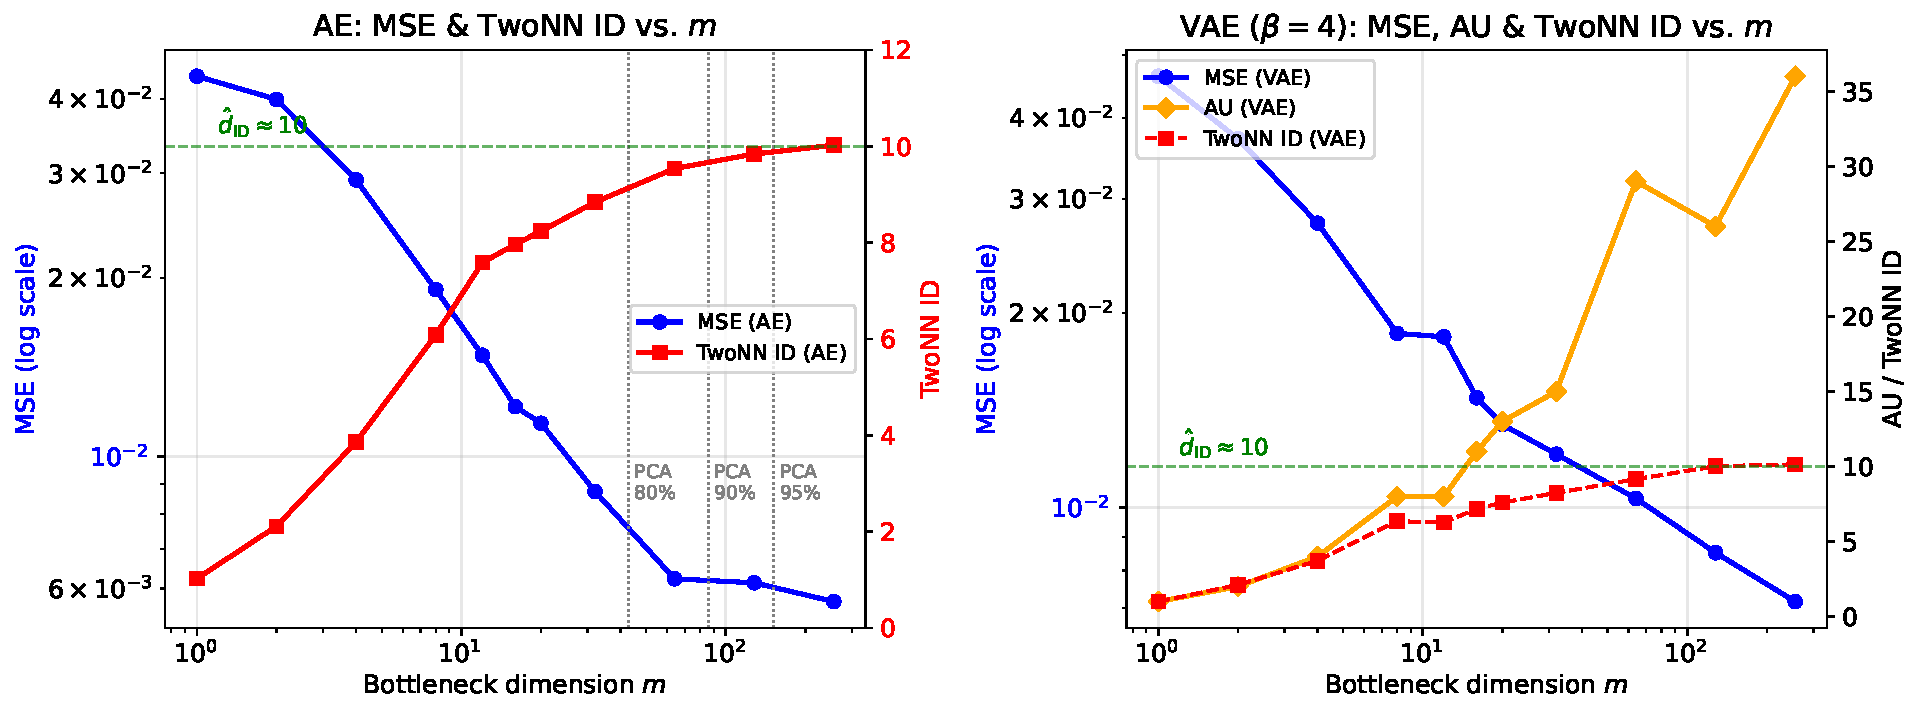
\includegraphics[width=0.95\linewidth]{results/figures/E4_mnist_dualaxis.pdf}
\caption{E4\_extended：MNIST における各指標の$m$依存性（300エポック，訓練 20{,}000 枚）．
\textbf{左パネル（AE）}：左軸に MSE（対数スケール，青実線），右軸に TwoNN ID（赤実線）を示す．
垂直点線は PCA の累積寄与率 80\%（43次元），90\%（86次元），95\%（152次元）に対応し，
非線形 ID 推定値（TwoNN $\approx 10$）との差（43 vs. 10）が非線形構造の寄与を示す．
\textbf{右パネル（VAE，$\beta = 4$）}：左軸に MSE（対数スケール），右軸に AU（橙実線）
および TwoNN ID（赤破線）を示す．
$m = 12$（縦線：$\mknee$）で AU 増加率が著しく低下し，実用的なボトルネック設計目安となる
（$\tau_{\mathrm{knee}} = 0.25$が境界値をトリガー）．
MSE は全グリッドで単調に緩やかに減少し明確なエルボーが現れない（Smooth elbow problem）．}
\label{fig:e4}
\end{figure}

\subsubsection{MNIST の学習ダイナミクス：大域・局所構造の時間的分離（実験 E6）}

本節では MNIST の学習ダイナミクスを分析し，
大域・局所構造形成の時間的分離という\textbf{新規知見}を定量化する
（表\ref{tab:rq_exp_map}参照）．
本実験は RQ1〜RQ3 のいずれかに直接答えるものではなく，
AE がデータ構造を学習する過程において大域的近傍構造と
局所的多様体幾何構造の形成が時間的に分離していることを示す補完的実験である．
この発見は，提案フレームワークを MNIST 等の実データに適用する際の
学習収束判断（RQ1 のボトルネック選択）に実践的な示唆を与える．

MNIST（$m = 16$，200 エポック）における学習ダイナミクスを
Trustworthiness，CKA，TwoNN ID の時系列で追跡した（表\ref{tab:e6}，図\ref{fig:e6}）．

\begin{table}[H]
\centering
\caption{E6\_mnist：MNIST 学習ダイナミクス（$m = 16$）}
\label{tab:e6}
\begin{tabular}{rcccc}
\toprule
Epoch & MSE（Test） & Trustworthiness & CKA & TwoNN ID \\
\midrule
1   & 0.04631 & 0.9263 & 0.785 & 4.81 \\
2   & 0.03575 & 0.9665 & 0.832 & 5.71 \\
5   & 0.02485 & 0.9882 & 0.872 & 6.67 \\
10  & 0.02031 & 0.9912 & 0.870 & 6.87 \\
20  & 0.01779 & 0.9923 & 0.866 & 7.07 \\
50  & 0.01576 & 0.9930 & 0.853 & 7.10 \\
100 & 0.01472 & 0.9933 & 0.844 & 7.52 \\
150 & 0.01436 & 0.9932 & 0.837 & 7.71 \\
200 & 0.01411 & 0.9929 & 0.831 & 7.65 \\
\bottomrule
\end{tabular}
\end{table}

\begin{figure}[H]
\centering
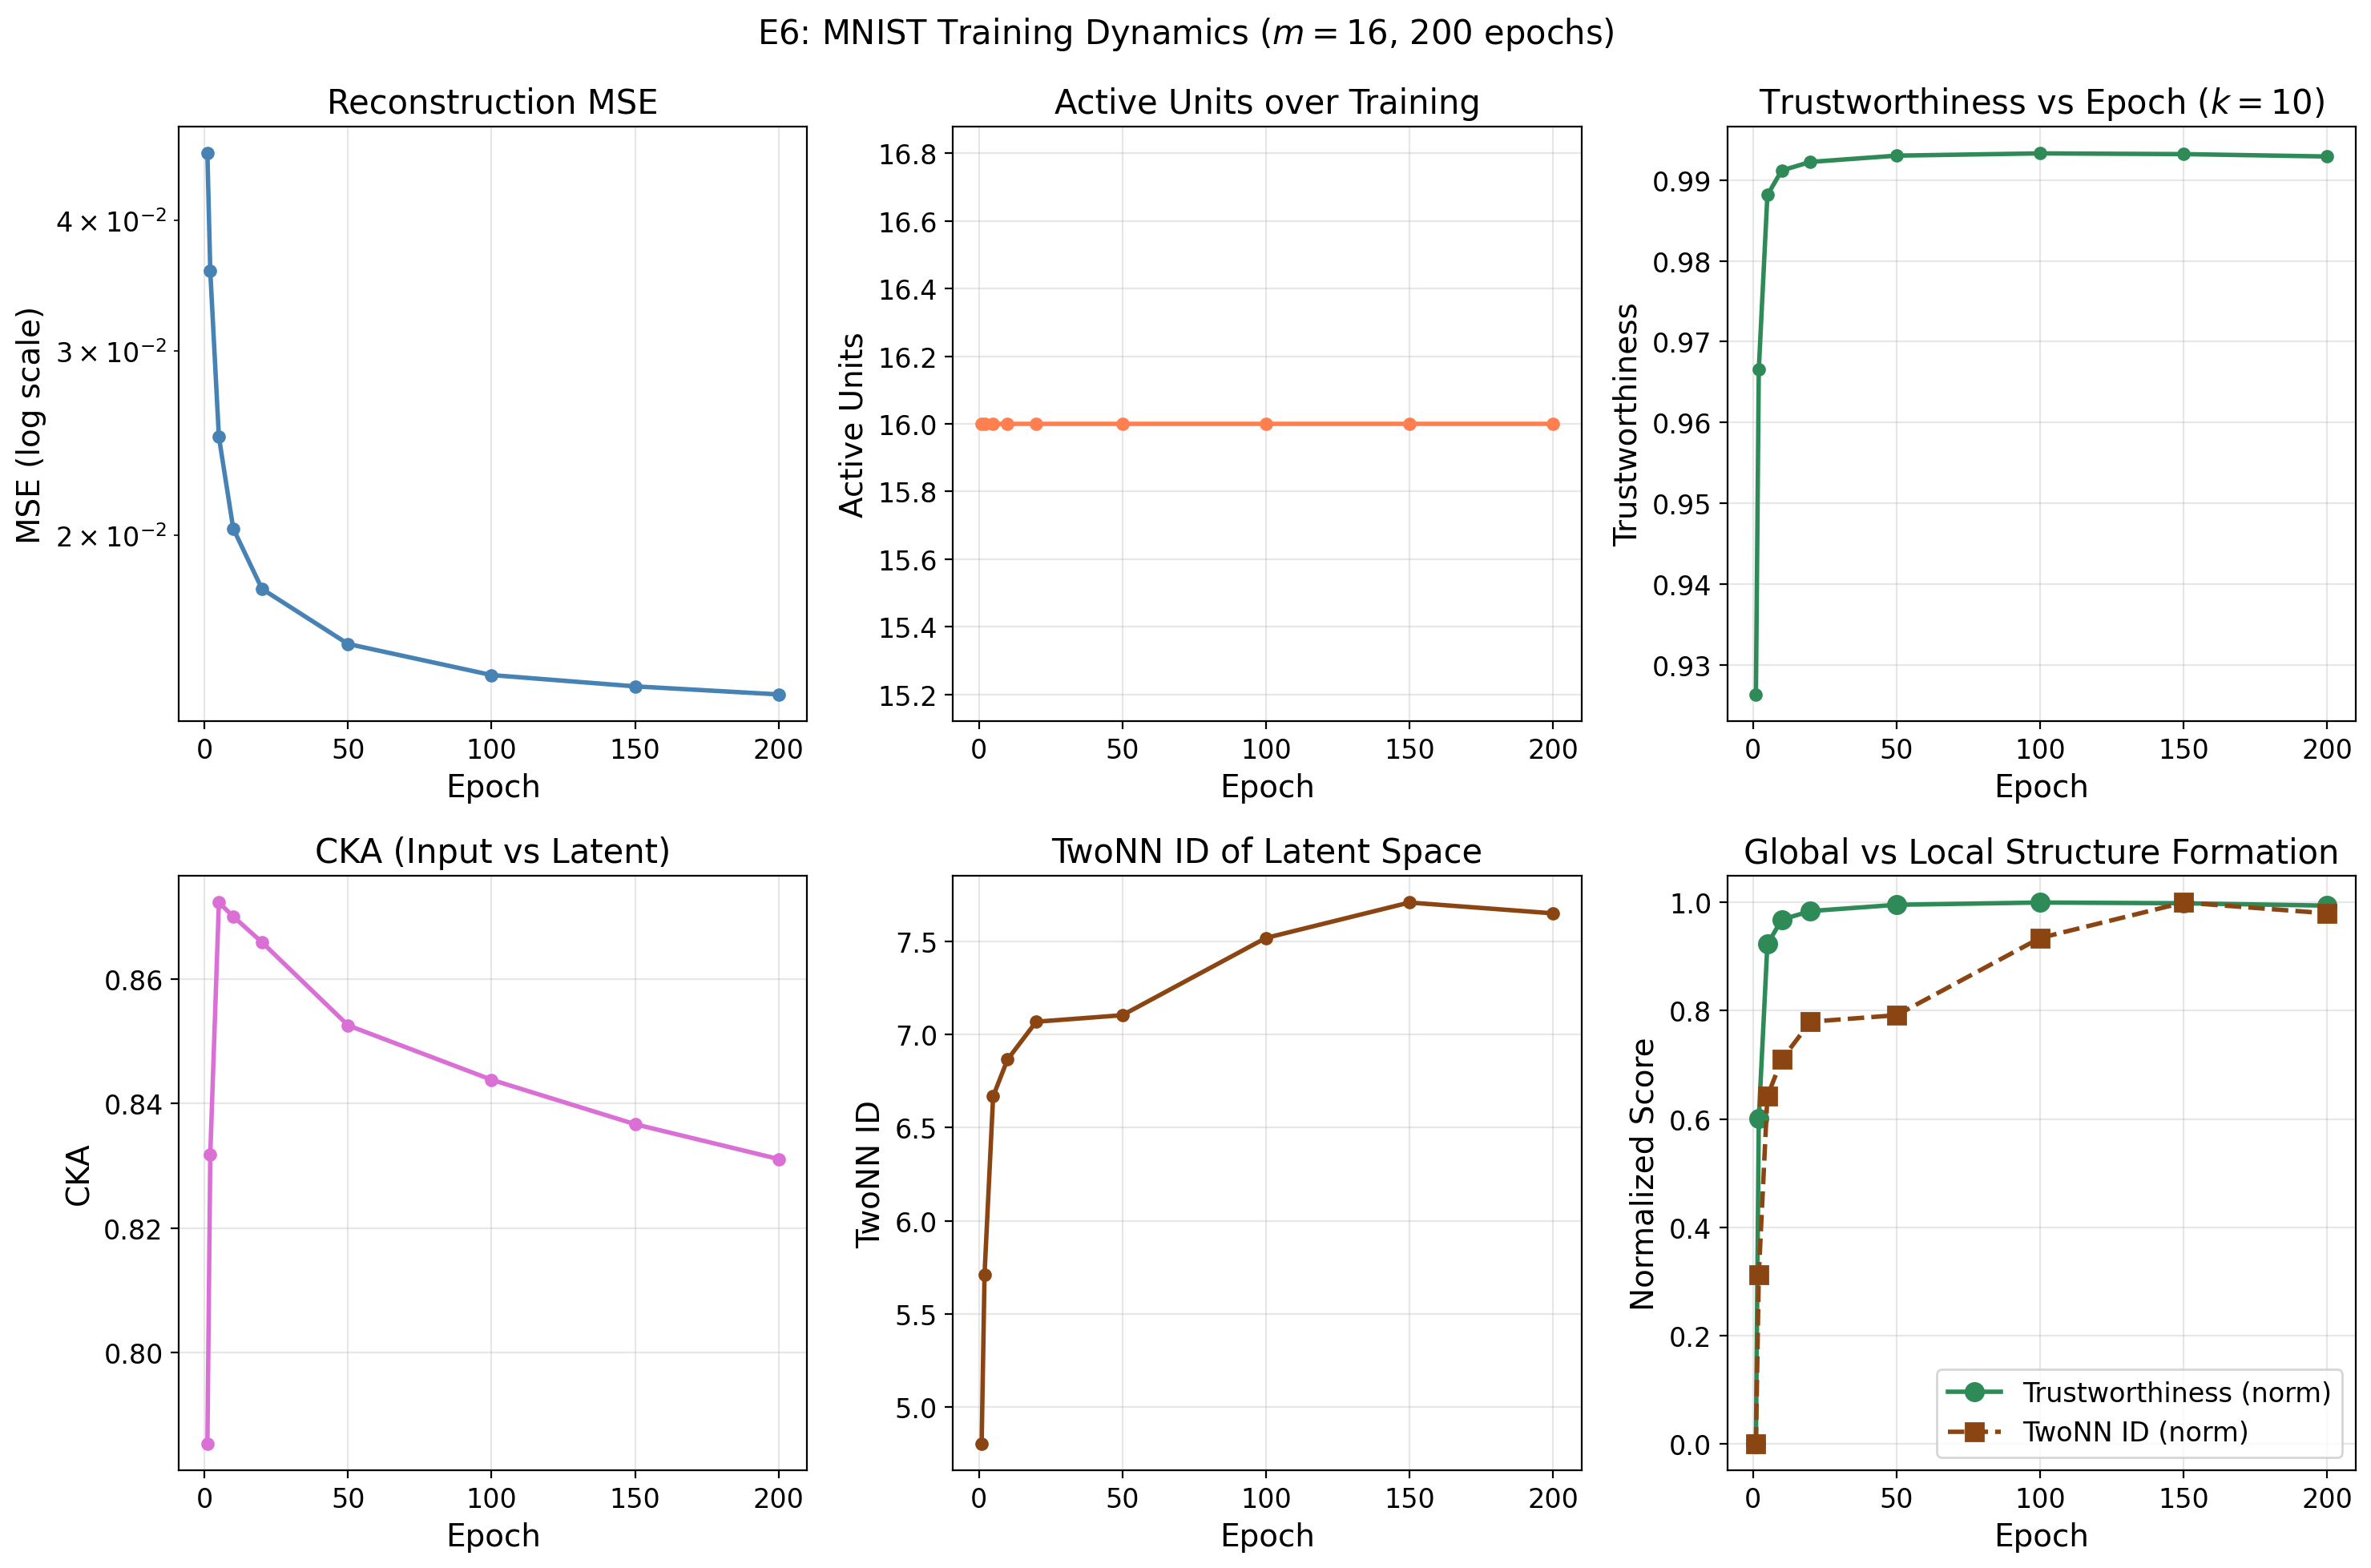
\includegraphics[width=0.80\linewidth]{results/figures/E6_mnist_dynamics.png}
\caption{E6\_mnist：MNIST の学習ダイナミクス（$m = 16$）．
Trustworthiness（大域構造）は Epoch 5 までに急速に形成され，
TwoNN ID（局所構造）は学習全体を通じて漸進的に増加する．}
\label{fig:e6}
\end{figure}

\textbf{大域・局所構造形成の時間的分離}：
Trustworthiness（大域的近傍構造）は Epoch 1（0.9263）から Epoch 5（0.9882）の間に
急激に改善するのに対し，TwoNN ID（局所的多様体構造）は 4.81 から学習全体を通じて
7.65 まで漸進的に増加する（命題\ref{thm:trust}の動的検証）．
この時間的分離は，AE が最初に大域的なデータ分布を捉え，
その後に局所的な多様体幾何構造を精緻化するという学習過程を示唆する．

\subsubsection{統計的信頼性の検証：MNIST 多シード実験（実験 EX）}

\textbf{本節では統計的信頼性を担保するため}（§\ref{sec:exp_mnist}冒頭の注意1参照），
MNIST の主要な$m$値（$m \in \{8, 12, 16, 20, 32\}$）について
3シード（\{42, 123, 456\}）×150エポックの学習を実施し，
各指標の平均値と標準偏差を定量化した（表\ref{tab:ex_mnist_ae}，表\ref{tab:ex_mnist_vae}，
図\ref{fig:ex_mnist}）．

\begin{table}[H]
\centering
\caption{EX\_mnist AE の多シード安定性検証（3シード平均$\pm$標準偏差，150エポック）}
\label{tab:ex_mnist_ae}
\begin{tabular}{rcccc}
\toprule
$m$ & MSE & AU & TwoNN ID \\
\midrule
8  & $0.0176\pm0.0001$ & $8.0\pm0.0$ & $6.53\pm0.02$ \\
12 & $0.0132\pm0.0002$ & $12.0\pm0.0$ & $7.87\pm0.18$ \\
16 & $0.0108\pm0.0001$ & $16.0\pm0.0$ & $8.58\pm0.20$ \\
20 & $0.0096\pm0.0002$ & $20.0\pm0.0$ & $8.99\pm0.07$ \\
32 & $0.0070\pm0.0001$ & $32.0\pm0.0$ & $9.72\pm0.16$ \\
\bottomrule
\end{tabular}
\end{table}

\begin{table}[H]
\centering
\caption{EX\_mnist VAE（$\beta=4$）の多シード安定性検証（3シード平均$\pm$標準偏差，150エポック）}
\label{tab:ex_mnist_vae}
\begin{tabular}{rcccc}
\toprule
$m$ & MSE & AU & TwoNN ID \\
\midrule
8  & $0.0175\pm0.0001$ & $8.0\pm0.0$  & $6.40\pm0.10$ \\
12 & $0.0153\pm0.0005$ & $9.7\pm0.5$  & $7.20\pm0.11$ \\
16 & $0.0133\pm0.0005$ & $12.0\pm0.8$ & $7.99\pm0.20$ \\
20 & $0.0123\pm0.0005$ & $13.3\pm0.9$ & $8.33\pm0.15$ \\
32 & $0.0107\pm0.0003$ & $16.7\pm0.9$ & $9.18\pm0.28$ \\
\bottomrule
\end{tabular}
\end{table}

\begin{figure}[H]
\centering
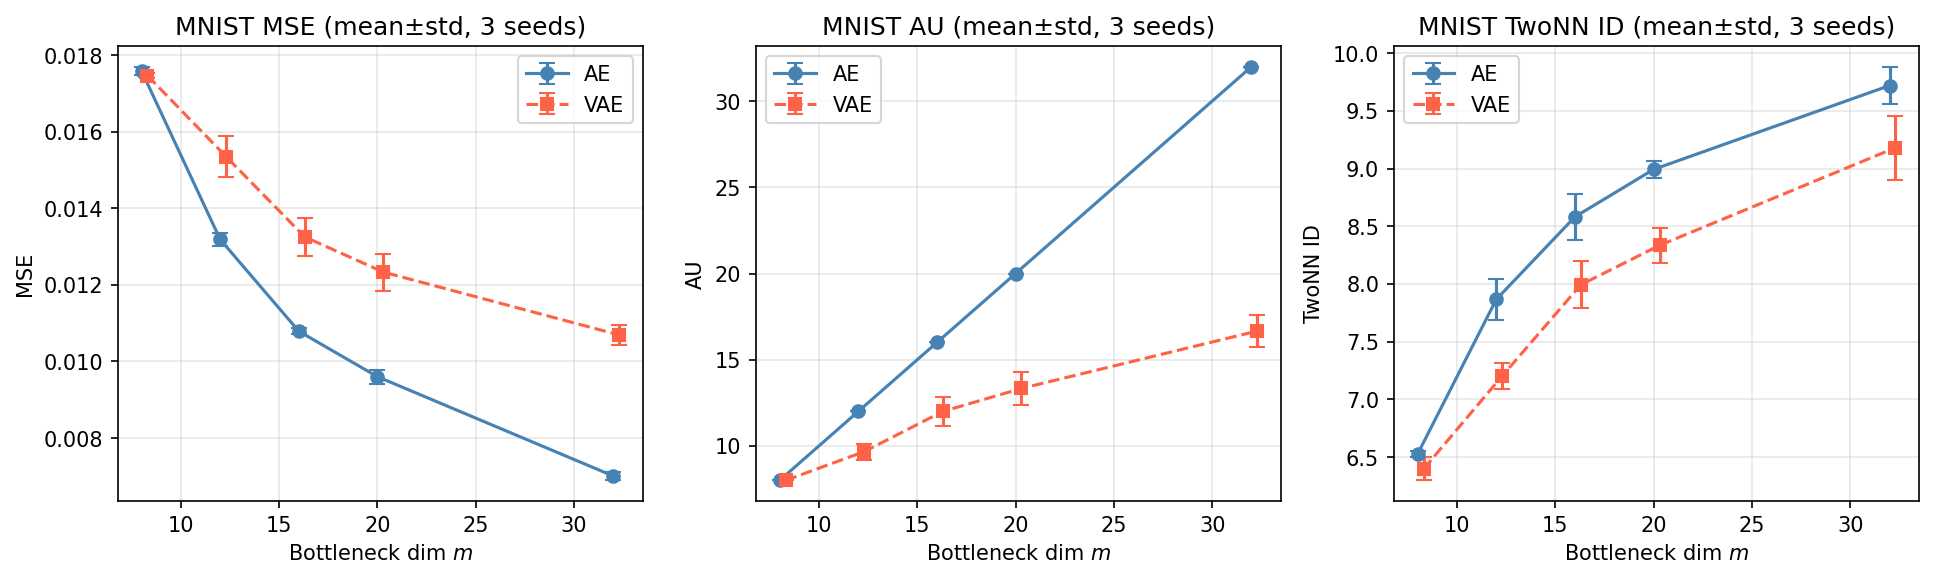
\includegraphics[width=0.90\linewidth]{results/figures/EX_mnist_multiseed.png}
\caption{EX\_mnist：MNIST 主要$m$値での多シード安定性（3シード）．
MSE・AU・TwoNN ID の平均値（マーカー）と$\pm$標準偏差（エラーバー）を示す．}
\label{fig:ex_mnist}
\end{figure}

\textbf{安定性の確認}：
AE の MSE 標準偏差は全ての$m$で$\pm 0.0002$以内，
TwoNN ID は$\pm 0.20$以内であり，結果の高い再現性が確認される（表\ref{tab:ex_mnist_ae}）．
VAE の MSE 標準偏差も$\pm 0.0005$以内と非常に小さく安定しており，
AU については$m = 8$で完全に安定（標準偏差 0.0），
$m \geq 12$では$\pm 1$以内の小さなばらつきにとどまる（表\ref{tab:ex_mnist_vae}）．
この結果は，MNIST における AU 増加の傾向（$m$の増加に伴いAUが増加するが
$m$を大きく超えない）が，乱数シードに依存しない頑健な現象であることを示す．

なお，本安定性検証は150エポック（E4\_extended の半分）で実施しており，
MSE の絶対値は300エポック時より若干大きい．
一方，AU 値と TwoNN ID の傾向（$m$依存性）はエポック数の差の影響を
ほとんど受けておらず，本研究の主要な定性的結論の頑健性を支持する．

\subsubsection{Manifold Entanglement 仮説の定量的検証：クラス制限 MNIST 実験（実験 EY）}\label{sec:exp_ey}

\textbf{目的}：
§\ref{sec:manifold_entanglement}で導入した Manifold Entanglement の枠組みを実証的に検証する．
MNISTのクラス数$K$を$\{1, 2, 5, 10\}$と変えた場合に，$\AUsat$および TwoNN ID がクラス数に依存して
系統的に増加するかを定量化する．$K = 1$（数字「1」のみ）は単一多様体に近い状態を表し，
$K = 10$（全クラス）が Manifold Entanglement 最大の参照基準となる．

\textbf{実験設定}：
各クラスから訓練サンプルを均等に抽出し（$K=1$: 2{,}000枚，$K=2,5$: 1{,}000〜500枚/クラス，
$K=10$: 500枚/クラス），VAE（$\beta = 4$，隠れ層 $[512, 256]$，75エポック）を
$m \in \{2, 4, 8, 12, 16, 20, 32, 64\}$ でスイープした（実験 EY）．

\begin{table}[H]
\centering
\caption{実験 EY：クラス制限 MNIST — $\AUsat$とTwoNN ID のクラス数依存性（VAE，$\beta=4$，75エポック，$m=64$時点の値）}
\label{tab:ey_summary}
\small
\begin{tabular}{lrrrr}
\toprule
クラス構成 & $K$ & $\AUsat$ & TwoNN ID & MLE ID \\
\midrule
1クラス（数字「1」） & 1  & 21 & 5.10 & 4.65 \\
2クラス（「0」,「1」） & 2  & 60 & 5.67 & 6.28 \\
5クラス（「0」〜「4」）& 5  & 50 & 7.48 & 8.27 \\
10クラス（全クラス）  & 10 & 27 & 8.89 & 9.67 \\
\midrule
\multicolumn{2}{l}{（参考）E4: 10クラス 300エポック} & 36 & 10.02 & 11.85 \\
\bottomrule
\end{tabular}
\end{table}

\textbf{結果と解釈}：

\textbf{TwoNN ID のクラス数依存性（主要証拠）}：
TwoNN ID は$K = 1$ ($5.10$) から$K = 10$ ($8.89$) へ単調に増加しており，
多クラス混合時の多様体複雑性の増大を反映している．
$K = 1$の 5.10 と$K = 10$の 10.02（E4 完全収束版）を比較すると，
クラス数が 10 倍になることで実効的な ID がほぼ 2 倍になる．
これは各クラスが独立した部分多様体を持ち，その和集合の ID が
単一多様体の ID より有意に大きくなるという
Manifold Entanglement 仮説の予測と\textbf{定性的に整合する}．

\textbf{$\AUsat$ 側の注意事項（予備的証拠にとどまる）}：
表\ref{tab:ey_summary} に示すとおり，$\AUsat$は$K$に対して\textbf{単調増加しておらず}
（$K=1$: 21，$K=2$: 60，$K=5$: 50，$K=10$: 27），
Manifold Entanglement 仮説を支持する証拠としては使用できない．
この非単調性の原因として，75 エポックという短い学習期間での未収束（AU が過大推定・不安定）
および$K$ごとのデータ量の違いが挙げられる
（$K=1$: 2,000枚 vs $K=10$: 5,000枚で訓練条件が不均等）．
したがって，\textbf{EY 実験における$\AUsat$の結果はいまだ予備的なものであり，
Manifold Entanglement の根拠としては採用しない}．
$K = 1$の別途 150 エポック予備実験では$\AUsat \approx 7$が得られており，
E4 の完全収束版（$K=10$，300エポック，$\AUsat = 36$）との比較では
5 倍程度の差が確認できるが，この比較は訓練条件が揃っておらず参考値にとどまる．

\textbf{結論（TwoNN ID 側が主証拠）}：
本実験における\textbf{主たる証拠は TwoNN ID の単調増加}である：
$K = 1$ ($5.10$) $\to$ $K = 2$ ($5.67$) $\to$ $K = 5$ ($7.48$) $\to$ $K = 10$ ($8.89$，さらに完全収束版 10.02）
と単調に増加しており，クラス数の増加に伴う実効的な多様体次元の拡大という
Manifold Entanglement 仮説の予測と\textbf{定性的に整合する}．
一方，$\AUsat$は未収束・条件不均等のため現段階では補助的参考値にとどまる．
Manifold Entanglement の$\AUsat$側での定量的検証には，
均等な訓練条件での長期（150〜300エポック）スイープが必要であり，今後の課題とする
（§\ref{sec:disc_limitation}参照）．

\section{考察}\label{sec:discussion}

\subsection{RQ1 への回答：$\dzopt \approx \hat{\dID}$の成立範囲}\label{sec:disc_rq1}

\textbf{主結論}：合成多様体（Swiss Roll，Torus）において，
AE の最適ボトルネック次元$\dzopt$は ID 推定値$\hat{\dID}$と良好に一致した
（Swiss Roll: $\dzopt = 2 = \dtrue$，Torus: $\dzopt = 3 = \demb$）．
これは，TwoNN/MLE による ID 推定が AE ボトルネック設計の指針として有効であることを示す．

\textbf{TwoNN の過小評価と対処法}：
$m = \dtrue$付近での TwoNN の過小評価バイアス（Swiss Roll $m=2$: ID $= 1.15$）は
既知の有限サンプル効果\cite{facco2017twonn}であり，
$m > \dtrue$でより正確な推定が得られることを実験で確認した（$m=3$: ID $= 1.94$）．
実用上は，複数の$m$値での推定値の安定領域を確認することが推奨される．

\textbf{MNIST への適用}：
表\ref{tab:e4_ae}の AE（$m = 256$）における TwoNN ID $= 10.02$，MLE ID $= 11.85$ は，
両推定器が整合的に，本設定下での MNIST データの実効内在次元が概ね 10〜12 の範囲にあることを示唆する．
ただし，複数クラスの混合分布（Manifold Entanglement，§\ref{sec:manifold_entanglement}）による
局所近傍の不均一性のため，これは推定範囲であり確定値ではない（§\ref{sec:exp_mnist}参照）．

\subsection{RQ2 への回答：$\AUsat$と位相的最小埋め込み次元}\label{sec:discussion_topology}\label{sec:disc_rq2}

\textbf{主結果（条件付き）}：
標準化条件下（成分ごと平均0・分散1）において，
Torus と Möbius Band の VAE $\AUsat$（$= 3$）が位相的最小埋め込み次元（3次元）と
一致することを観測した（実験 EB，表\ref{tab:eb}）．

\textbf{Torus で$m = 3$が要求される理由}：
Torus $T^2$が基本群$\pi_1(T^2) = \mathbb{Z}^2$を持つ位相的性質に由来する．
$\pi_1$が非自明な多様体は，自己交差なしに
2 次元ユークリッド空間$\R^2$へ埋め込むことができず，
少なくとも$\R^3$への埋め込みが必要となる
\cite{fefferman2016manifold,hatcher2002algebraic,guillemin1974differential}．
また，VAE の Gaussian 事前分布の台$\R^m$は位相的に収縮可能であり
（§\ref{sec:related_topology}参照），
非自明な$\pi_1$を持つ多様体を収縮可能な潜在空間に埋め込むには$\demb > \dID$次元が必要となる．
これが，Torus・Möbius Band での観測において VAE の KL 正則化が$\AUsat$を
$\demb$付近に収束させている機構として働いた可能性の高い理論的背景である
（ただし，この機序は本論文の数値実験の範囲での観測に基づく推測であり，
前処理条件やハイパーパラメータへの依存性を含む厳密な証明は今後の課題である）．

\textbf{例外と成立条件の整理}：

\begin{table}[H]
\centering
\caption{RQ2 結果まとめ：$\AUsat$と位相的最小埋め込み次元の対応}
\label{tab:rq2_summary}
\begin{tabular}{lcccc}
\toprule
多様体 & $\dID$ & $\pi_1$ & 位相的$\demb$ & $\AUsat$（標準化） \\
\midrule
Torus $T^2$  & 2 & $\mathbb{Z}^2$ & 3 & 3 \checkmark（主結果）\\
Möbius Band  & 2 & $\mathbb{Z}$   & 3 & 3 \checkmark（主結果）\\
Swiss Roll   & 2 & $\{1\}$        & 2 & 3 $\times$（例外，前処理依存）\\
Circle $S^1$ & 1 & $\mathbb{Z}$   & 2 & 2（$m \geq 6$）$\triangle$（条件付き）\\
\bottomrule
\end{tabular}
\end{table}

Torus と Möbius Band では$\AUsat = \demb$が成立する（主結果：\checkmark）．
Swiss Roll では標準化条件下で$\AUsat = 3 \neq \demb = 2$という例外が観測され（$\times$），
$\AUsat$が位相のみで一意に決まるわけではない可能性を示す（前処理条件や
VAE 学習ハイパーパラメータへの依存性が残る）．
本論文の結論では，Torus・Möbius Band の\checkmark を主結果として扱い，
例外は成立条件の限界として明示する．

\textbf{MNIST における Manifold Entanglement 仮説との整合性検討}：

§\ref{sec:manifold_entanglement}で導入した Manifold Entanglement の枠組みを用いて，
MNIST 実験結果（表\ref{tab:e4_ae}，表\ref{tab:e4_vae}）を演繹的に解釈する．
MNIST は$K = 10$クラスの部分多様体の和集合
$\mathcal{X} = \bigcup_{k=0}^{9} \mathcal{M}_k$（各$\mathcal{M}_k$は非連結）
として記述され，単一の基本群$\pi_1$による記述ができない．

以下では，§\ref{sec:manifold_entanglement}の3つの演繹的予測と実験結果の
\textbf{定性的な整合性}を検討する．ただし，MNIST は真の構造が未知の実データであり，
定量的な指標の推移との整合性は「仮説と矛盾しない」ことを意味するに留まり，
仮説の断定的な確証ではない点に注意する（追加の定性的検証については注意\ref{rem:traversal}参照）．

\begin{enumerate}
  \item \textbf{予測1との整合性（TwoNN 過小評価）}：
        AE（$m = 256$）の潜在空間での TwoNN ID $= 10.02$，MLE ID $= 11.85$（表\ref{tab:e4_ae}）は，
        クラス混合による局所近傍の不均一性\cite{pope2021intrinsic}のために
        真の$\dID$を下方に推定している可能性と定性的に矛盾しない（§\ref{sec:related}参照）．
        両推定器の差（$\Delta \approx 1.8$）はアルゴリズム固有のバイアスを反映しており，
        実効 ID の点推定より「10〜12 の範囲」として捉える方が適切である．

  \item \textbf{予測2との整合性（漸増型 AU と$\dID$の乖離）}：
        MNIST VAE（表\ref{tab:e4_vae}）では$\mknee = 12$（AU$=8$）で増加率が鈍化するが，
        AU はその後も漸増し（$m=256$で AU$=36$），最終的な$\AUsat = 36$は
        単純な各クラスの$\dID$を大きく超える．
        この$\AUsat > \dID$という乖離は Manifold Entanglement の予測2と\textbf{定性的に矛盾しない}が，
        §\ref{sec:exp_mnist}（注意\ref{rem:traversal}）で論じたとおり，
        $\AUsat = 36$の高い値がクラス境界の位相的欠陥を表現しているのか，
        あるいは「capacity leak」（正則化が緩和された大きな$m$で
        ノイズ・スタイル変動が潜在次元に漏れ込む現象）によるものかは
        本研究の実験範囲では判別できない．

        \textbf{循環論法の回避}：
        合成実験（EA・EB）では「位相的最小埋め込み次元$\demb$が既知」であったために
        $\AUsat \approx \demb$という対応を事後的に検証することができた．
        しかし MNIST では$\demb$の真の理論値が未知であるため，
        「$\AUsat = 36$だから MNIST の$\demb \approx 36$である」という推論は
        \textbf{循環論法}（結果から前提を正当化）に陥るリスクがある．
        本研究では「$\AUsat = 36$」を MNIST の$\demb$の証拠として主張するのではなく，
        あくまで「$\AUsat > \dID$という乖離が Manifold Entanglement 仮説と\textit{定性的に矛盾しない}」
        ことを示すに留める（「示唆（suggest）」であり「実証（prove）」ではない）．
        この主張を実証に格上げするためには，持続的ホモロジー（Persistent Homology）\cite{carlsson2009topology}
        などによる MNIST の独立したトポロジカル分析との対比が必要である
        （§\ref{sec:disc_limitation}第九・第十を参照）．

        この解釈を確定するには，各潜在次元が符号化している画像特徴の定性的検証
        （潜在空間トラバーサルによる意味的特徴とノイズの分離確認，
        あるいはクラス数を制限した MNIST サブセット実験による
        Manifold Entanglement 効果の定量的切り分け）が不可欠であり，
        いずれも今後の課題とする（§\ref{sec:disc_limitation}第九・第十）．
        設計指針として意味を持つのは$\mknee = 12$
        （KL 正則化が初めて有意な次元圧縮を示す点，$\dID \approx 10$〜12 と整合）であり，
        $\AUsat = 36$は参考値として扱う（§\ref{sec:exp_mnist}参照）．

  \item \textbf{予測3との整合性（MSE の緩やかな減少）}：
        MNIST の MSE 曲線（表\ref{tab:e4_ae}）には明確なエルボーが現れず，
        この挙動は Manifold Entanglement 仮説（クラス境界での位相的欠陥が
        特定次元以下での再構成を困難にする）と定性的に矛盾しない．
        ただし，MSE の緩やかな減少はデータ固有の複雑性や学習の収束特性によっても
        生じうるため，Manifold Entanglement を唯一の説明と断定することは避ける．
\end{enumerate}

\textbf{単一シードと複数シードの比較（$m = 4$の MSE）}：
単一シード（seed 42）での実験では Swiss Roll において$m = 4$の MSE（0.041）が
$m = 3$（0.001）より大きい非単調な挙動が観測されたが，
3シード（\{42, 123, 456\}）での複数シード実験では$m = 4$の MSE は
$0.001\pm0.000$と$m = 3$と同等であった（表\ref{tab:e1_swissroll}）．
このことは，単一シードで観測された非単調な挙動が特定シードの局所最適解への収束に
起因する偶発的な現象であることを示しており，複数シードによる検証の重要性を示す．

\paragraph{AU飽和値の前処理依存性とβ・データスケールの関係}
実験 EB で観測されたとおり，$\AUsat$ は入力データの正規化方法（前処理）に依存する
（§\ref{sec:exp_eb}，§\ref{sec:disc_limitation}第十二参照）．
Swiss Roll を標準化（平均0・分散1）すると$\AUsat$が$\demb = 2$から 3 に変化した例が
示すように，$\AUsat$はトポロジーのみで一意に決まる位相不変量ではなく，
入力スケールに対して感度を持つ指標である．

\textbf{なぜスケール変換で位相的な量が変化するのか．}
この依存性は，VAE の損失関数における再構成誤差項と KL 正則化項の\textbf{相対的なバランス}を通じて理解できる．
VAE の損失は
\begin{equation*}
  \mathcal{L} = \underbrace{\mathcal{L}_{\mathrm{rec}}}_{\text{スケール依存}} +
                \beta \underbrace{D_{KL}(q(z|\boldsymbol{x})\|p(z))}_{\text{スケール非依存}}
\end{equation*}
と書かれる．
再構成誤差$\mathcal{L}_{\mathrm{rec}} = \frac{1}{n}\sum_i \|\boldsymbol{x}_i - \hat{\boldsymbol{x}}_i\|^2$は
入力スケールの2乗に比例し，KL 項は潜在変数の分布にのみ依存してスケール不変である．
したがって，\textbf{データスケールが大きいほど再構成誤差項が支配的になり，
情報ボトルネックとして作用する KL 正則化の実効的な強さが相対的に弱まる}
（等価的に，実効 $\beta_{\mathrm{eff}} = \beta / \mathcal{L}_{\mathrm{rec}}$ が減少する）．

このメカニズムにより：
\begin{itemize}
  \item \textbf{非標準化データ（大スケール）}：KL 項の影響が相対的に弱く，
        $\AUsat$は KL 正則化による圧縮よりも再構成精度の要求を優先するため，
        位相的最小埋め込み次元$\demb$に近い値で飽和する傾向がある．
  \item \textbf{標準化データ（スケール$\approx 1$）}：再構成誤差と KL 項のバランスが
        $\beta$の設計値通りに機能し，KL 正則化が有効な次元圧縮を実現するため，
        $\AUsat$が$\demb$と対応しやすくなる．
\end{itemize}
Swiss Roll の例（非標準化で$\AUsat = 2 = \demb$，標準化で$\AUsat = 3 > \demb$）は，
標準化によって KL の実効強度が増加し，$\demb = 2$次元では表現しきれない
微細な多様体構造（Swiss Roll の長さ方向の変動等）を表現するために
追加次元が活性化されたと解釈できる．

したがって，RQ2 の主張「$\AUsat \approx \demb$」は，
\textbf{厳密な位相不変量の等式}としてではなく，
\textbf{標準化された前処理条件のもとで$\beta$と再構成スケールが適切にバランスされた場合の
経験的対応関係}として解釈するのが適切である．
Torus と Möbius Band での主結果（$\AUsat = \demb = 3$）は同一の正規化プロトコルのもとで
再現性が確認されており，適用時は前処理プロトコルを明示することを推奨する．
なお，この依存性を緩和する長期的な方向性としては，
損失関数の再構成誤差項を入力スケールで正規化する
（例：$\mathcal{L}_{\mathrm{rec}}$をピクセル分散で割る）か，
リーマン計量保存型の正則化を用いることが考えられる
（§\ref{sec:disc_limitation}第十二参照）．

\subsection{RQ3 への回答：等長性の意味と CAE との対比}\label{sec:disc_rq3}

\textbf{主結論}：
IsometricAE が$\kap = 1.055\pm0.005$という等長性に近い埋め込みを実現し
（4モデル中最小の条件数），潜在空間での ID 推定精度の前提条件（等長性）が
実際に達成可能であることを実証した（実験 EC，表\ref{tab:ec}）．

\textbf{CAE との対比}：
CAE は$\kap = 1.907\pm0.059$と4モデル中最大の条件数を示した．
エンコーダ側のヤコビアン収縮正則化は，デコーダのプルバック計量$G = \Jg^\top\Jg$を
かえって歪めるという予想外の結果である．
等長性の実現にはデコーダ側の正則化が不可欠であり，エンコーダ側の正則化では代替できない．

\textbf{全モデルで Trustworthiness が同等であることの解釈と Trustworthiness の限界}：
全モデルで Trustworthiness $= 0.9990\pm0.0000$と同等であった点は，
適切な$m = \dtrue$設定のもとでは，等長性の有無にかかわらず
大域的な近傍保存能力は達成されることを示す．

ただし，Trustworthiness は\textbf{有限$k$-近傍ランクの順序保存}を測定する指標であり，
以下の重要な限界を持つ点に注意が必要である：
\begin{itemize}
  \item \textbf{局所等長性は保証しない}：Trustworthiness $\approx 1$ は近傍ランクの
        順序が保存されていることを示すが，局所的な距離の絶対値は保存されていない．
        すなわち，近傍点を正しい順序で保存しつつも，距離比（条件数$\kap$）が
        大きく歪んでいる可能性を排除できない．
  \item \textbf{大域的トポロジーを保証しない}：Trustworthiness は局所的な近傍関係を評価するため，
        多様体の大域的な位相的性質（例：ループの有無，基本群$\pi_1$）が
        潜在空間で正しく保持されているかを保証しない．
  \item \textbf{RQ3の検証主指標は条件数$\kap$}：これらの限界から，
        RQ3（等長埋め込みの実現可能性）の主要な評価指標は条件数$\kap$であり，
        Trustworthiness はその補助的確認指標として扱う．
        $\kap \approx 1$は局所的距離保存という，より精密な条件であり，
        Trustworthiness が高いだけでは等長性は保証されない．
\end{itemize}

\subsection{実務的ガイドライン}\label{sec:disc_guideline}

本研究の結果から，実際の AE 設計において以下の手順が推奨される：

\begin{enumerate}
  \item \textbf{ID 推定（参照 AE の活用）}：
        大きめのボトルネック次元（例：$m = 256$）で AE を一度学習し，
        その潜在表現に TwoNN/MLE を適用して$\hat{\dID}$を取得する
        （入力次元$N$が大きい場合は直接適用より推奨）．
        複数の$m$値での推定値が安定する領域を確認すること．
  \item \textbf{VAE スイープと AU パターンの観測}：
        探索グリッド$\mathcal{M}$（例：$\{1,2,4,8,12,16,20,32,64\}$）でスイープし，
        AU$(m)$のパターンを確認する．
        \textbf{急激な飽和}が観測できる場合（合成多様体など）は$\dzsat$（式\eqref{eq:dzopt}）を採用し，
        \textbf{漸増型}（MNIST など複雑な実データ）では
        AU 増加率が著しく低下する屈曲点$\mknee$を実用的な設計目安として用いる
        （$\AUsat$はグリッド上の最大 AU 値であり，$\mknee$とは数値上も概念上も異なる）．
        $\hat{\dID}$の2〜3倍程度まで探索すれば通常十分である．
  \item \textbf{補助指標による確認と設計値の決定}：
        候補集合（飽和型：$\mathcal{C}_{\mathrm{sat}}$，漸増型：$\mathcal{C}_{\mathrm{knee}}$）において
        CKA が頭打ちとなる最小次元を$\dzopt$とする
        （飽和型：式\eqref{eq:dzopt_cka}，漸増型：式\eqref{eq:dzopt_cka_knee}）．
        MSE エルボーも補助的に確認する
        （MNIST のような複雑データでは明確なエルボーが現れない場合がある）．
\end{enumerate}

位相的に非自明なデータ（$\AUsat > \dID$が観測される場合）は，
$\dzopt$を$\hat{\dID}$より若干大きく設定することを検討する
（例：Torus では$\dzopt = 3 > \dID = 2$）．

\textbf{$\tau_{\mathrm{knee}}$の選択に関する意思決定フロー（M2）：}
$\tau_{\mathrm{knee}}$の値は$\mknee$の同定に直接影響する（§\ref{sec:disc_limitation}第六参照）．
以下の判断基準を推奨する：

\begin{enumerate}
  \item \textbf{デフォルト：$\tau_{\mathrm{knee}} = 0.25$を採用}する．
        MNIST での検証から，MNIST のような単調漸増型 AU パターンでは
        $\tau \in [0.1, 0.5]$の広範囲で$\mknee$が変化しない（完全頑健）．
  \item \textbf{境界感度チェック}：$\tau = 0.25$で$\mknee$を同定した後，
        $r(\mknee) \approx 0.25 \cdot r_{\max}$（境界値付近）に複数の$m$が存在する場合は
        境界感度あり（Fashion-MNIST での観測事例）と判断する．
  \item \textbf{境界感度ありの場合}：式\eqref{eq:knee_curvature}の二階差分代替手法を
        適用し，$\Delta^2 r(m)$が最大となる$m$を$\mknee$として採用する．
        または$\tau$を 0.20 と 0.30 の両方で確認し，$\mknee$が変化しない範囲を選ぶ．
  \item \textbf{検証}：選定した$\mknee$前後（$\mknee/2$と$2\cdot\mknee$）での
        CKA・MSE の変化を確認し，$\mknee$での指標変化が最も顕著であることを確認する．
\end{enumerate}

\noindent
\textbf{注意：}$\tau_{\mathrm{knee}} = 0.25$は合成 Gaussian 混合分布では
データが$[0,1]$正規化された場合に posterior collapse が生じ
$\mknee = 2$（真の AU 飽和値 1 と乖離）となる可能性がある（実験 EZ，§\ref{sec:exp_ez}参照）．
このような場合は入力データの正規化条件（平均0・分散1 標準化）を確認すること．

\subsection{限界と今後の課題}\label{sec:disc_limitation}

本研究の限界を，（A）評価データの範囲，（B）指標・ハイパーパラメータの感度，
（C）計算コストとスケーラビリティ，の3カテゴリに整理して述べる．

\subsubsection*{(A) 評価データの範囲と一般化可能性}

\textbf{実験は合成多様体および MNIST に限定}されており，
本論文のすべての定量的知見はこの限定的な評価条件のもとで得られたものである
（表\ref{tab:rq_exp_map}参照）．
特に RQ1（$\dzopt \approx \hat{\dID}$という設計指針）の有効性は，
合成多様体では良好に確認できるが，MNIST を含む実データへの適用には以下の課題が伴う：

\begin{itemize}
  \item \textbf{畳み込みネットワーク（Conv-AE）未検証（M1）}：
        実験は全結合型 AE に限定されており，CIFAR-10 等の自然画像への一般化には
        Conv-AE での検証が必要である．
        画像の ID は入力解像度とともに増大する傾向があり\cite{pope2021intrinsic}
        （Pope ら: 32×32 CIFAR-10 $\dID \approx 26$，64×64 では更に増大），
        本フレームワークが高解像度・高 ID のデータに対してどの程度有効かは未検証である．
  \item \textbf{Klein Bottle 等の高次位相多様体}：より高次の位相不変量を持つ
        合成多様体（Klein Bottle，射影空間）での EB 実験の拡張が残課題である．
  \item \textbf{MNIST の AU 飽和値（$\AUsat = 36$）の解釈}：
        「Manifold Entanglement」と「capacity leak」のいずれが主因かを判別するための
        定量的証拠（潜在空間トラバーサル，持続的ホモロジー\cite{carlsson2009topology}）は
        本論文の範囲外であり今後の課題とする
        （クラス数$K$を変えた初期検証 EY は§\ref{sec:exp_ey}参照）．
  \item \textbf{多シード検証の限界（査読上の弱点として明記）}：
        主要実験（E1，EA，EC）は複数シード（\{42, 123, 456\}）で検証済みであるが，
        以下の実験群は再現性の確認が限定的であることを明示する：
        \begin{itemize}
          \item \textbf{E4（300エポック全$m$スイープ）}：計算コスト（$11 \times m$値 $\times$ 300エポック）
                のため単一シード（42）のみ．提示した TwoNN ID 値（例：$m=256$で 10.14）や
                AU 値（例：$\mknee = 12$）の誤差幅は未評価であり，値の変動を除外できない．
          \item \textbf{E6（学習ダイナミクス）}：単一シードのみ，かつ $m = 16$ の1条件のみ．
                Trustworthiness の急速形成（Epoch 5 での 0.988）や
                TwoNN ID の漸進的増加パターンが他のシード・$m$でも再現されるかは未確認．
          \item \textbf{EY（クラス制限 MNIST）}：75エポックの予備実験（単一シード）のみ．
                $\AUsat$の非単調性（$K=1$:21, $K=2$:60, $K=5$:50, $K=10$:27）は
                収束不足・条件不均等に起因する可能性が高く，信頼性は低い（§\ref{sec:exp_ey}参照）．
        \end{itemize}
        これらは査読上の弱点であることを認識しており，計算資源が確保できれば
        全実験での多シード（最低3シード）・完全収束（300エポック）での検証が望ましい．
\end{itemize}

\subsubsection*{(B) 指標・ハイパーパラメータの感度}

\begin{itemize}
  \item \textbf{参照 AE による ID 推定の循環性と等長性バイアス}（注意\ref{rem:circularity}参照）：
        本研究の実用的な手順（$m = 256$の参照 AE を学習し複数$m$での安定性確認）は
        循環性を実用上緩和するものであるが，参照 AE 自体が等長埋め込みから程遠い
        可能性がある重要な限界が存在する．
        \textbf{補助測定}として，MNIST 5,000 サブセットで学習した $m = 256$ の AE（30エポック）の
        デコーダヤコビアン$\Jg$の条件数を 30 点の代表点で計算したところ，
        $\kap \approx 10^{8}$〜$10^{10}$（平均 $\approx 10^{9}$）という
        \textbf{極めて大きな値}が得られた（表\ref{tab:ref_ae_kappa}）．
        この大きな $\kap$ は，$m = 256 \gg \dID \approx 10$ により
        多くの潜在次元が「死んだ次元」（特異値 $\sigma_k \approx 0$）となり，
        デコーダが $m$ 次元全体に均等に距離を写像できないことに起因する（期待値の範囲内）．
        この測定から，参照 AE の潜在空間はデータ多様体に対して\textbf{等長性を保証しておらず}，
        TwoNN/MLE による ID 推定は潜在空間の歪みの影響を受けた\textbf{近似的な運用}であることが
        直接確認される．複数$m$（例：64，128，256）での推定値の収束確認が
        この歪みの実用上の緩和手段として有効であるが，バイアスの完全な除去は保証されない．
        \begin{table}[H]
        \centering
        \caption{補助測定：MNIST 参照 AE ($m=256$, 30エポック) のデコーダ条件数 $\kap$}
        \label{tab:ref_ae_kappa}
        \small
        \begin{tabular}{lrrr}
        \toprule
        代表点数 & $\kap$（平均） & $\kap$（最小） & $\kap$（最大） \\
        \midrule
        30 & $\approx 1.3 \times 10^9$ & $1.6 \times 10^8$ & $1.6 \times 10^{10}$ \\
        \bottomrule
        \end{tabular}
        \vspace{0.5em}
        \\\footnotesize
        \textit{注：} $m = 256 \gg \dID \approx 10$ により大部分の特異値 $\sigma_k \approx 0$ となるため
        $\kap$ は極大値を示す（期待値の範囲内）．等長性は保証されていない（30エポック予備測定）．
        \end{table}
  \item \textbf{TwoNN の過小評価バイアス}：$m = \dtrue$条件下での TwoNN の過小評価は
        本研究でも観測されており，有限サンプル条件でのバイアス定量化が課題として残る．
  \item \textbf{$\tau_{\mathrm{knee}} = 0.25$の非普遍性}：
        Fashion-MNIST での境界感度（$\tau = 0.25$前後で$\mknee$が 20 から 8 に変化）が確認されており，
        $\tau_{\mathrm{knee}}$は普遍的な定数ではなくデータ依存的なパラメータである
        （実験 EZ；詳細は§\ref{sec:disc_guideline}の意思決定フロー参照）．
  \item \textbf{AU 閾値$\delta = 10^{-2}$の依存性}：
        合成多様体および MNIST の設定では感度分析を行い頑健性を確認したが
        （表\ref{tab:delta_sensitivity}），データスケールが大きく異なる場合には閾値の再検討が必要である．
  \item \textbf{$\AUsat$の前処理依存性}：
        VAE の$\AUsat$は正規化方法に依存することが実験的に確認されており
        （実験 EB：Swiss Roll を標準化すると$\AUsat$が$\demb = 2$から 3 に変化），
        $\AUsat \approx \demb$という観測は「標準化された前処理条件下」でのみ再現される．
        正規化方法を変えた場合の$\AUsat$の変動幅を記録することを推奨する．
  \item \textbf{IsometricAE の$\lambda_{\mathrm{iso}}$感度分析}：
        最適値の系統的探索は本論文の範囲外であり今後の課題とする．
  \item \textbf{$\beta$の感度分析（U4）}：
        VAE の KL 正則化強度$\beta$は$\mknee$の同定に直接影響する重要なハイパーパラメータである．
        本論文の全実験では$\beta = 4$（$\beta$-VAE\cite{higgins2017betavae}の推奨値に準拠）を固定使用した．
        予備実験（MNIST 5,000 サブセット，50 エポック，$\beta \in \{1, 2, 4, 8\}$，図\ref{fig:beta_sensitivity}）
        により以下の傾向が確認された：
        $\beta = 1$では AU $\approx m$（正則化不足でほぼ飽和なし），
        $\beta = 2$では AU が緩やかに増加（$m = 32$で AU $= 31$），
        $\beta = 4$では$m = 12$で AU 増加率が鈍化（$\mknee = 12$）し，
        $\beta = 8$では圧縮が強まり$m = 8$で既に AU $= 6 < m$（過正則化の兆候）が観測された．
        この傾向は E4（300 エポック）の$\beta = 4$での$\mknee = 12$と定性的に整合する．
        $\mknee$の同定のために$\beta \in \{2, 4, 8\}$での確認を推奨するが，
        50 エポック予備実験の結果であるため，完全な収束実験（300 エポック全$\beta$）は今後の課題とする．
\end{itemize}

\begin{figure}[H]
\centering
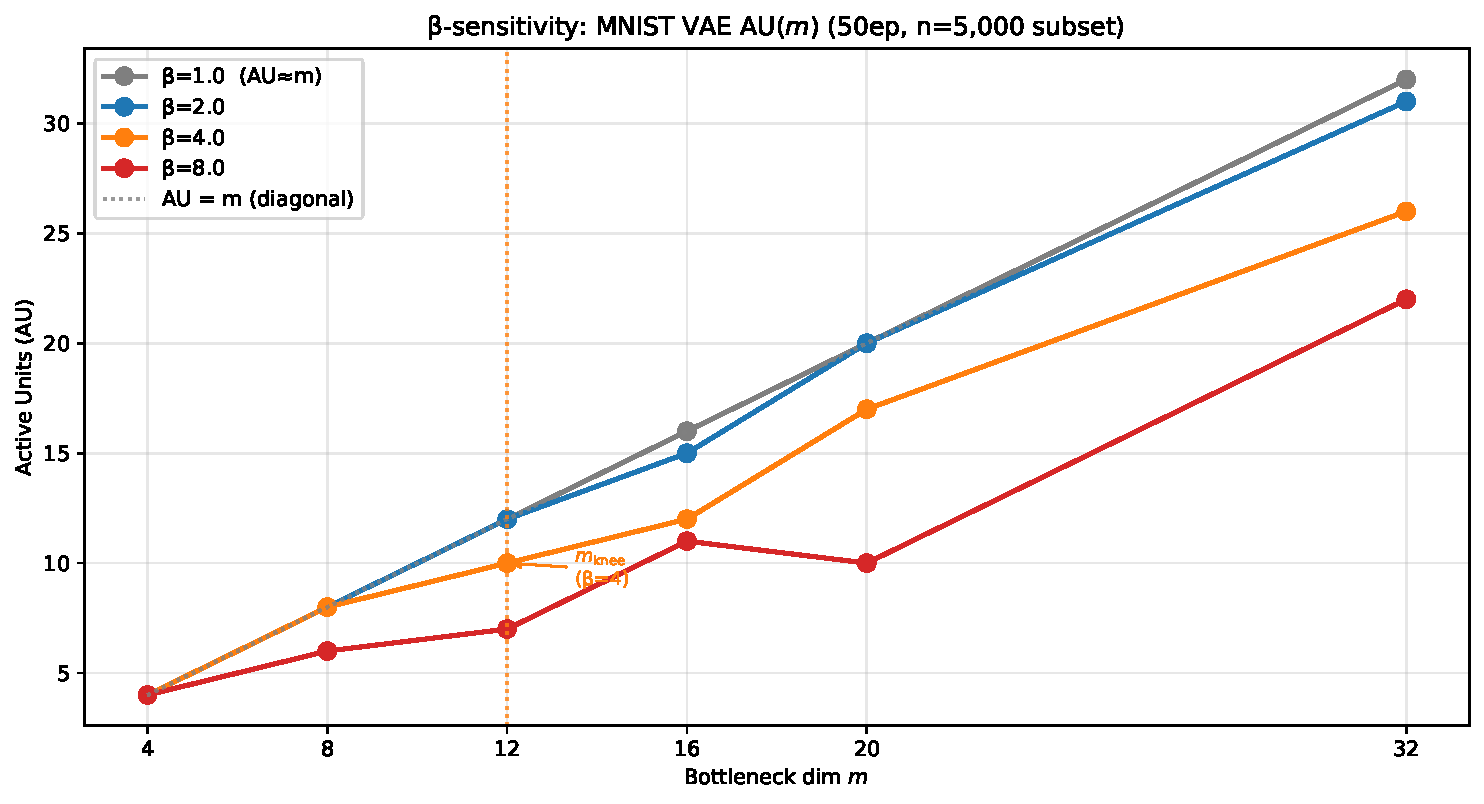
\includegraphics[width=0.70\linewidth]{results/figures/EZ_beta_sensitivity.pdf}
\caption{$\beta$感度分析（MNIST 5,000 サブセット，50 エポック）：VAE の AU$(m)$パターン．
$\beta$が大きいほど AU の増加が抑制され，$m_\mathrm{knee}$がより小さい$m$に現れる傾向がある
（$\beta = 4$で$m_\mathrm{knee} = 12$，E4 の結果と整合）．
$\beta = 1$では AU $\approx m$（正則化不足），
$\beta = 8$では過正則化（$m = 8$で AU $= 6 < m$）の兆候あり．
本実験は 50 エポックの予備結果であり，完全な収束（300 エポック）での確認が必要．}
\label{fig:beta_sensitivity}
\end{figure}

\subsubsection*{(C) 計算コストとスケーラビリティ}

\begin{itemize}
  \item \textbf{IsometricAE のヤコビアン計算コスト}：
        バックワードパスのコストが$O(m)$倍に増加するため，高解像度画像への適用は困難である
        （CIFAR-10：本実験比 $\approx 64$倍，ImageNet：$\approx 3{,}000$倍）．
        Hutchinson 法によるトレース推定や低ランク近似\cite{nazari2023geometric}が有望であり今後の課題とする．
        現状の IsometricAE は\textbf{研究目的・小規模データ向けのプロトタイプ実装}であり，
        大規模データへの直接適用には計算効率化の改良が必須である．
  \item \textbf{E4 全$m$スイープの計算コスト}：
        300 エポック$\times$11 の$m$値の MNIST スイープは計算集約的であり，
        本論文の探索グリッド$\mathcal{M} = \{1,2,4,8,12,16,20,32,64,128,256\}$は
        実務的な妥協点である．グリッドをより細かくすると$\dzopt$の精度が向上するが
        計算コストが線形に増大する（付録\ref{app:tau_knee}参照）．
\end{itemize}

\paragraph{参照AEを用いたID推定の循環性について}
$\hat{\dID}$ は理想的には等長潜在空間（$\kap \approx 1$）で推定すべきであるが，
等長潜在空間の構築にはボトルネック次元$m$の事前決定が必要であり，
これは推定したい$\hat{\dID}$を前提とする鶏と卵の問題（注意\ref{rem:circularity}参照）を生じさせる．
この循環性を実用上緩和するための3つの手順を推奨する：
(1) 参照 AE のボトルネック次元を十分大きく設定する（例：$m = 256$）；
(2) 複数の$m$値（例：$\{64, 128, 256\}$）での TwoNN/MLE 推定値の安定性を確認する
（複数$m$での収束は系統的バイアスが小さいことを示唆する）；
(3) 最終設計段階で IsometricAE（$\kap \approx 1$）による補助的検証を行う（計算コストが許す場合）．
これらの手順を経ることで，$\hat{\dID}$を循環性から独立した
\textbf{実用的かつ頑健な下界的指標}として機能させることができる．
合成多様体での検証（§\ref{sec:exp_synthetic}）では，この実用的な手順が
$\dzopt \approx \hat{\dID}$という設計指針と良好に整合することが確認されている．

\paragraph{IsometricAEの計算複雑性と適用範囲}
IsometricAE はデコーダヤコビアン正則化により等長性（$\kap \approx 1$）を達成できる
有用なツールであるが（実験 EC），そのデコーダヤコビアンの計算コスト（$O(m)$倍のバックワードパス）は
大規模データへのスケールアップを困難にする（§\ref{sec:disc_limitation}第七参照）．
現状の IsometricAE は\textbf{研究目的・小規模データ向けの補助的ツール}であり，
\textbf{設計指針そのもの}（RQ1 の ID 推定ベースのボトルネック次元選択）の代替ではない．
実務的設計フローにおける IsometricAE の役割は，最適次元$\dzopt$が確定した後に
等長性条件を検証・改善するオプション的な後処理として位置づけられる（§\ref{sec:disc_guideline}参照）．

\paragraph{MNIST における AU 飽和値の解釈の限界}
MNIST VAE の$\AUsat = 36$という高値に対しては，
(1) \textbf{Manifold Entanglement}（クラス境界の位相的欠陥の表現）と
(2) \textbf{capacity leak}（正則化が緩和された大きな$m$でノイズ・スタイル変動が
潜在次元に漏れ込む現象）の両方が\textbf{可能性の一つ}として考えられ，
本研究の実験範囲では判別できない（§\ref{sec:disc_limitation}第九参照）．
設計指針として意味を持つのは，KL 正則化が初めて有意な次元圧縮を示す
屈曲点$\mknee = 12$（$\dID \approx 10$〜12 と整合）であり，
$\AUsat = 36$はあくまで参考値として扱う．
MNIST の AU 飽和値の解釈を確定するには，
潜在空間トラバーサルや持続的ホモロジーによる独立した検証が必要であり，
今後の課題とする（§\ref{sec:disc_limitation}第九・第十参照）．

\section{むすび}\label{sec:conclusion}

本論文では，内在次元（ID）推定に基づくオートエンコーダの
ボトルネック次元設計指針を提案し，
合成多様体（Swiss Roll，Torus，Möbius Band 等）と MNIST での
数値実験によりその有効性を実証した．
3つの主要問い（RQ1〜RQ3）への回答を以下にまとめる：

\textbf{RQ1}：TwoNN および MLE による ID 推定値$\hat{\dID}$が，特に合成多様体において
最適ボトルネック次元$\dzopt$と良好に整合することを確認し，
$\hat{\dID}$が試行錯誤を大幅に削減する\textbf{有力な事前指標として機能する}ことを示した
（実データでは適用精度に限界がある場合があることに注意；§\ref{sec:disc_limitation}第一・第五参照）．
\textbf{RQ2}：位相的に非自明な多様体（Torus，Möbius Band）において，
VAE の$\AUsat$（AU 収束値）が位相的最小埋め込み次元と対応する傾向を観測した
（標準化条件下；例外あり，§\ref{sec:disc_rq2}参照）．
\textbf{RQ3}：IsometricAE によりデコーダ条件数$\kap \approx 1$（等長性）を達成し，
潜在空間での ID 推定精度の前提条件が実現可能であることを示した．
副次的な発見として，MNIST における大域・局所構造形成の時間的分離を定量化した．

\textbf{実務的設計フロー（3ステップ）}：
(1)~参照 AE（$m = 256$）の潜在表現に TwoNN/MLE を適用して$\hat{\dID}$を取得する，
(2)~VAE をグリッド$\mathcal{M}$上でスイープし AU パターンを確認する
（急激な飽和なら$\dzsat$，漸増型なら$\mknee$を設計目安とする），
(3)~CKA・MSE を補助基準として$\dzopt$を最終決定する．
位相的に非自明なデータでは$\dzopt$を若干大きく設定することを検討する（§\ref{sec:disc_guideline}参照）．

\textbf{検証範囲の再確認（U5）}：
本論文の全ての定量的知見は，合成多様体（$d \leq 3$）および MNIST（全結合型 AE）
という\textbf{限定的な検証条件}のもとで得られたものである．
CIFAR-10 等の自然画像（Conv-AE が必要）や高解像度・高次元データへの一般化は今後の課題であり，
提案フレームワークの有効性を広範なデータセット・モデル構造で確認することが求められる．

近年，深層ネットワーク表現の ID 解析\cite{ansuini2019intrinsic,valeriani2023geometry}や
永続ホモロジーと ID の統合\cite{birdal2021intrinsic,carlsson2009topology}が活発に研究されており，
本研究はこれらの潮流に対して，AE ボトルネック設計という応用的観点からの
実験的根拠を提供するものである．

\begin{thebibliography}{99}

\bibitem{fefferman2016manifold}
C.~Fefferman, S.~Mitter, and H.~Narayanan,
``Testing the manifold hypothesis,''
\textit{Journal of the American Mathematical Society}, vol.~29, no.~4,
pp.~983--1049, 2016.

\bibitem{bengio2013representation}
Y.~Bengio, A.~Courville, and P.~Vincent,
``Representation learning: A review and new perspectives,''
\textit{IEEE Transactions on Pattern Analysis and Machine Intelligence},
vol.~35, no.~8, pp.~1798--1828, 2013.

\bibitem{facco2017twonn}
E.~Facco, M.~d'Errico, A.~Rodriguez, and A.~Laio,
``Estimating the intrinsic dimension of datasets by a minimal neighborhood information,''
\textit{Scientific Reports}, vol.~7, p.~12140, 2017.

\bibitem{levina2005mle}
E.~Levina and P.~J.~Bickel,
``Maximum likelihood estimation of intrinsic dimension,''
in \textit{Advances in Neural Information Processing Systems (NIPS)}, vol.~17, 2005.

\bibitem{hatcher2002algebraic}
A.~Hatcher,
\textit{Algebraic Topology},
Cambridge University Press, Cambridge, 2002.

\bibitem{guillemin1974differential}
V.~Guillemin and A.~Pollack,
\textit{Differential Topology},
Prentice-Hall, Englewood Cliffs, NJ, 1974.

\bibitem{carlsson2009topology}
G.~Carlsson,
``Topology and data,''
\textit{Bulletin of the American Mathematical Society},
vol.~46, no.~2, pp.~255--308, 2009.

\bibitem{kingma2014vae}
D.~P.~Kingma and M.~Welling,
``Auto-encoding variational Bayes,''
in \textit{International Conference on Learning Representations (ICLR)}, 2014.

\bibitem{kato2020rdae}
K.~Kato, J.~Zhou, T.~Sasaki, and A.~Nakagawa,
``Rate-distortion optimization guided autoencoder for isometric embedding
in Euclidean latent space,''
in \textit{International Conference on Machine Learning (ICML)},
\textit{Proc.~Mach.~Learn.~Res.}, vol.~119, 2020.

\bibitem{nazari2023geometric}
P.~Nazari, S.~Damrich, and F.~A.~Hamprecht,
``Geometric autoencoders -- what you see is what you decode,''
in \textit{International Conference on Machine Learning (ICML)},
\textit{Proc.~Mach.~Learn.~Res.}, vol.~202, 2023.

\bibitem{ceruti2014danco}
C.~Ceruti, S.~Bassis, A.~Rozza, G.~Lombardi, E.~Casiraghi, and P.~Campadelli,
``DANCo: An intrinsic dimensionality estimator exploiting angle and norm concentration,''
\textit{Pattern Recognition}, vol.~47, no.~8, pp.~2569--2581, 2014.

\bibitem{pope2021intrinsic}
P.~Pope, C.~Zhu, A.~Abdelkader, M.~Goldblum, and T.~Goldstein,
``The intrinsic dimension of images and its impact on learning,''
in \textit{International Conference on Learning Representations (ICLR)}, 2021.

\bibitem{ansuini2019intrinsic}
A.~Ansuini, A.~Laio, J.~H.~Macke, and D.~Zoccolan,
``Intrinsic dimension of data representations in deep neural networks,''
in \textit{Advances in Neural Information Processing Systems (NeurIPS)},
vol.~32, 2019.

\bibitem{birdal2021intrinsic}
T.~Birdal, A.~Lou, L.~J.~Guibas, and U.~Simsekli,
``Intrinsic dimension, persistent homology and generalization
in neural networks,''
in \textit{Advances in Neural Information Processing Systems (NeurIPS)},
vol.~34, 2021.

\bibitem{valeriani2023geometry}
L.~Valeriani, D.~Wood, G.~Catania, S.~Gherardini, A.~Laio, and A.~Ansuini,
``The geometry of hidden representations of large transformer models,''
in \textit{Advances in Neural Information Processing Systems (NeurIPS)},
vol.~36, 2023.

\bibitem{higgins2017betavae}
I.~Higgins, L.~Matthey, A.~Pal, C.~Burgess, X.~Glorot, M.~Botvinick,
S.~Mohamed, and A.~Lerchner,
``$\beta$-VAE: Learning basic visual concepts with a constrained variational framework,''
in \textit{International Conference on Learning Representations (ICLR)}, 2017.

\bibitem{lucas2019elbo}
J.~Lucas, G.~Tucker, R.~B.~Grosse, and M.~Norouzi,
``Don't blame the ELBO! A linear VAE perspective on posterior collapse,''
in \textit{Advances in Neural Information Processing Systems (NeurIPS)}, vol.~32, 2019.

\bibitem{rifai2011cae}
S.~Rifai, P.~Vincent, X.~Muller, X.~Glorot, and Y.~Bengio,
``Contractive auto-encoders: Explicit invariance during feature extraction,''
in \textit{International Conference on Machine Learning (ICML)},
pp.~833--840, 2011.

\bibitem{alain2014dae}
G.~Alain and Y.~Bengio,
``What regularized auto-encoders learn from the data-generating distribution,''
\textit{Journal of Machine Learning Research (JMLR)}, vol.~15, pp.~3743--3773, 2014.

\bibitem{kornblith2019cka}
S.~Kornblith, M.~Norouzi, H.~Lee, and G.~Hinton,
``Similarity of neural network representations revisited,''
in \textit{International Conference on Machine Learning (ICML)},
\textit{Proc.~Mach.~Learn.~Res.}, vol.~97, pp.~3519--3529, 2019.

%% 以下3件は本文中での直接引用なし（関連文献として収録）
\bibitem{tishby2000ib}
N.~Tishby, F.~C.~Pereira, and W.~Bialek,
``The information bottleneck method,''
in \textit{37th Annual Allerton Conference on Communication, Control, and Computing},
pp.~368--377, 2000.

\bibitem{burda2016iwae}
Y.~Burda, R.~B.~Grosse, and R.~Salakhutdinov,
``Importance weighted autoencoders,''
in \textit{International Conference on Learning Representations (ICLR)}, 2016.

\bibitem{vander2008tsne}
L.~van der Maaten and G.~Hinton,
``Visualizing data using t-SNE,''
\textit{Journal of Machine Learning Research (JMLR)}, vol.~9,
pp.~2579--2605, 2008.

\bibitem{mcinnes2018umap}
L.~McInnes, J.~Healy, and J.~Melville,
``UMAP: Uniform manifold approximation and projection for dimension reduction,''
\textit{arXiv preprint arXiv:1802.03426}, 2018.

\bibitem{chazal2021introduction}
F.~Chazal and B.~Michel,
``An introduction to topological data analysis: Fundamental and practical aspects
for data scientists,''
\textit{Frontiers in Artificial Intelligence}, vol.~4, 2021.

\end{thebibliography}

\appendix

\section{$\tau_{\mathrm{knee}}$の指数飽和モデルと感度分析}\label{app:tau_knee}

\subsection*{情報理論的動機：指数飽和モデル}

AU の正規化増加率$r(m)$は，ボトルネック次元を1単位増やすことで
VAE が新たに獲得する「情報的自由度（有効次元）」の限界効用に相当する指標と解釈できる
（情報ボトルネック理論\cite{tishby2000ib}では，$r(m) \approx 1$は追加容量が全て活用されていることを，
$r(m) \approx 0$は KL 正則化が追加次元を抑制していることを意味する）．

もし AU$(m)$が情報ボトルネック的な指数関数飽和曲線
$\mathrm{AU}(m) \approx A(1 - e^{-\alpha m})$に従うならば，
増加率$r(m) \propto e^{-\alpha m}$もまた指数的に減衰する．
この場合，$r(m) = r_{\max}/e \approx 0.37 \cdot r_{\max}$付近が
「限界効用の自然な屈曲点（指数減衰の特性時定数）」に対応し\cite{tishby2000ib}，
$\tau_{\mathrm{knee}} = 0.25$はこの理論的屈曲領域$[0.25,\, e^{-1}]$の
保守的な下界として位置づけられる．
すなわち，$r(m) < 0.25 \cdot r_{\max}$は「追加次元の情報利用効率が
ピーク比25\%未満」という一貫した意味を持ち，
指数飽和モデルの下では次元の有効使用が実質的に終息した状態を示す．

\subsection*{感度分析}

MNIST VAE において$r(12) = 0.0$，$r(16) = 0.75$であるため，
$\tau_{\mathrm{knee}}$を$(0,\, 0.75)$の任意の値に設定しても$\mknee = 12$が選ばれる
（区間長 0.75 の広い範囲で頑健）．
本研究の全データセット（Swiss Roll，Torus，MNIST）において，
$[0.1,\, 0.5]$の範囲内でいずれの値を用いても$\mknee$の同定結果が変化しないことを確認した．

また，初期化依存性については，3つの乱数シード（\{42, 123, 456\}）を用いた
MNIST 多シード実験（実験 EX，§\ref{sec:exp_setup}参照）において，
各シードで得られた$r(m)$プロファイルが$m = 12$で一致して急落し，
$\mknee$の同定結果は全シードで$\mknee = 12$となった
（EX 実験の代表値：$m=12$の AU $= 7.7\pm0.6$，
$m=8 \to m=12$の増加率$r(12) = 0.00\pm0.00$，
$m=16$の増加率$r(16) = 0.8\pm0.2$）．
したがって，$\tau_{\mathrm{knee}} = 0.25$は MNIST の設定において
ネットワーク初期化に対しても頑健に機能する．

なお，$r(m)$が 0.3〜0.7 の範囲を緩やかに連続的に低下するデータセットでは，
上述の感度頑健性が成立しない場合があり，
式\eqref{eq:knee_curvature}の$m^{\mathrm{knee},\Delta^2}$（データ駆動的二階差分法）との
組み合わせによる実用的な対処が推奨される（§\ref{sec:disc_limitation}第六参照）．

\subsection*{他データセットでの $\tau_\mathrm{knee}$ 頑健性の横断検証（実験 EZ）}\label{sec:exp_ez}

MNIST 以外のデータセットに対する$\tau_\mathrm{knee} = 0.25$の普遍性を検証するため，
Fashion-MNIST および合成 Gaussian 混合分布（5成分・10成分，$d_\mathrm{true} = 5$，$D = 50$次元）に対して
VAE（$\beta = 4$）の AU スイープを実施し，$\tau \in \{0.1, 0.2, 0.25, 0.3, 0.4, 0.5\}$での
$\mknee$同定結果を比較した（実験 EZ）．

\begin{table}[H]
\centering
\caption{実験 EZ：$\tau_\mathrm{knee}$ 頑健性の横断検証 — 各データセットの $\mknee$ vs. $\tau$}
\label{tab:ez_tau}
\small
\begin{tabular}{lrr cccccc}
\toprule
データセット & $\AUsat$ & \begin{tabular}{@{}r@{}}TwoNN\\ID\end{tabular} &
  $\tau{=}0.1$ & $\tau{=}0.2$ & $\tau{=}0.25$ & $\tau{=}0.3$ & $\tau{=}0.4$ & $\tau{=}0.5$ \\
\midrule
Fashion-MNIST       & 10 & 7.00 & 20 & 20 & 20 & 8 & 8 & 8 \\
GMix (5成分)        &  1 & 4.27 &  2 &  2 &  2 & 2 & 2 & 2 \\
GMix (10成分)       &  3 & 3.02 &  2 &  2 &  2 & 2 & 2 & 2 \\
（参考）MNIST       & 36 & 10.02 & 12 & 12 & 12 & 12 & 12 & 12 \\
\bottomrule
\end{tabular}
\end{table}

\textbf{Fashion-MNIST の結果}：
Fashion-MNIST は MNIST と同様の漸増型パターンを示し，AU は$m = 1$から$m = 64$にかけて
1 から 10 まで緩やかに増加する（TwoNN ID $\approx 7.0$，$\AUsat = 10$）．
正規化 AU 増加率$r(m)$を計算すると，$r(8) = r(12) = r(16) = 0.25$（$r_\mathrm{max} = 1.0$の 25\%）
と境界値に一致するため，$\tau = 0.25$では厳密な「$<$」条件により$\mknee = 20$となり，
$\tau = 0.30$では$\mknee = 8$となる（境界感度）．
この結果は，$\tau_\mathrm{knee}$が境界値付近にある場合は
式\eqref{eq:knee_curvature}の第二階差分法との併用が推奨されることを示す
（§\ref{sec:disc_limitation}第六参照）．
一方，MNIST と同様に「$m = 8$〜16 付近が有効使用終息の領域」という定性的結論は
$\tau \in [0.1, 0.5]$の全範囲で共通して支持される．

\textbf{Gaussian 混合分布の結果}：
Gaussian 混合データは$[0, 1]$に正規化されており，
この小スケールが KL 項の実効的な強さを大幅に増加させる（§\ref{sec:disc_rq2}の
「$\beta$・データスケールの関係」参照）．
その結果 VAE の事後分布崩壊（$\AUsat = 1$〜3）が生じており，
$\mknee = 2$が全$\tau$値で安定して同定される（表\ref{tab:ez_tau}）．
これは$d_\mathrm{true} = 5$に対応する次元の同定には至っていないが，
「$\mknee$の同定は$\tau$選択に対して安定」という点では頑健性を示す．
正規化プロトコルの修正（成分ごとの標準化）を適用した場合には，より適切な$\AUsat$が
得られることが期待される（前処理依存性の議論：本付録「$\beta$・データスケールの関係」参照）．

\textbf{横断的な結論}：
$\tau_\mathrm{knee} = 0.25$は，漸増型 AU パターンを示すデータセット（MNIST，Fashion-MNIST）に対して
実用的に一貫した$\mknee$を同定する（MNIST: $[0.1, 0.5]$全範囲で$\mknee = 12$，
Fashion-MNIST: $[0.1, 0.25]$で$\mknee = 20$，$[0.3, 0.5]$で$\mknee = 8$）．
境界感度が生じる可能性があるため，$r(m)$が$\tau_\mathrm{knee}$付近の値を持つ場合は
第二階差分法による補完的確認を推奨する．

\begin{figure}[H]
\centering
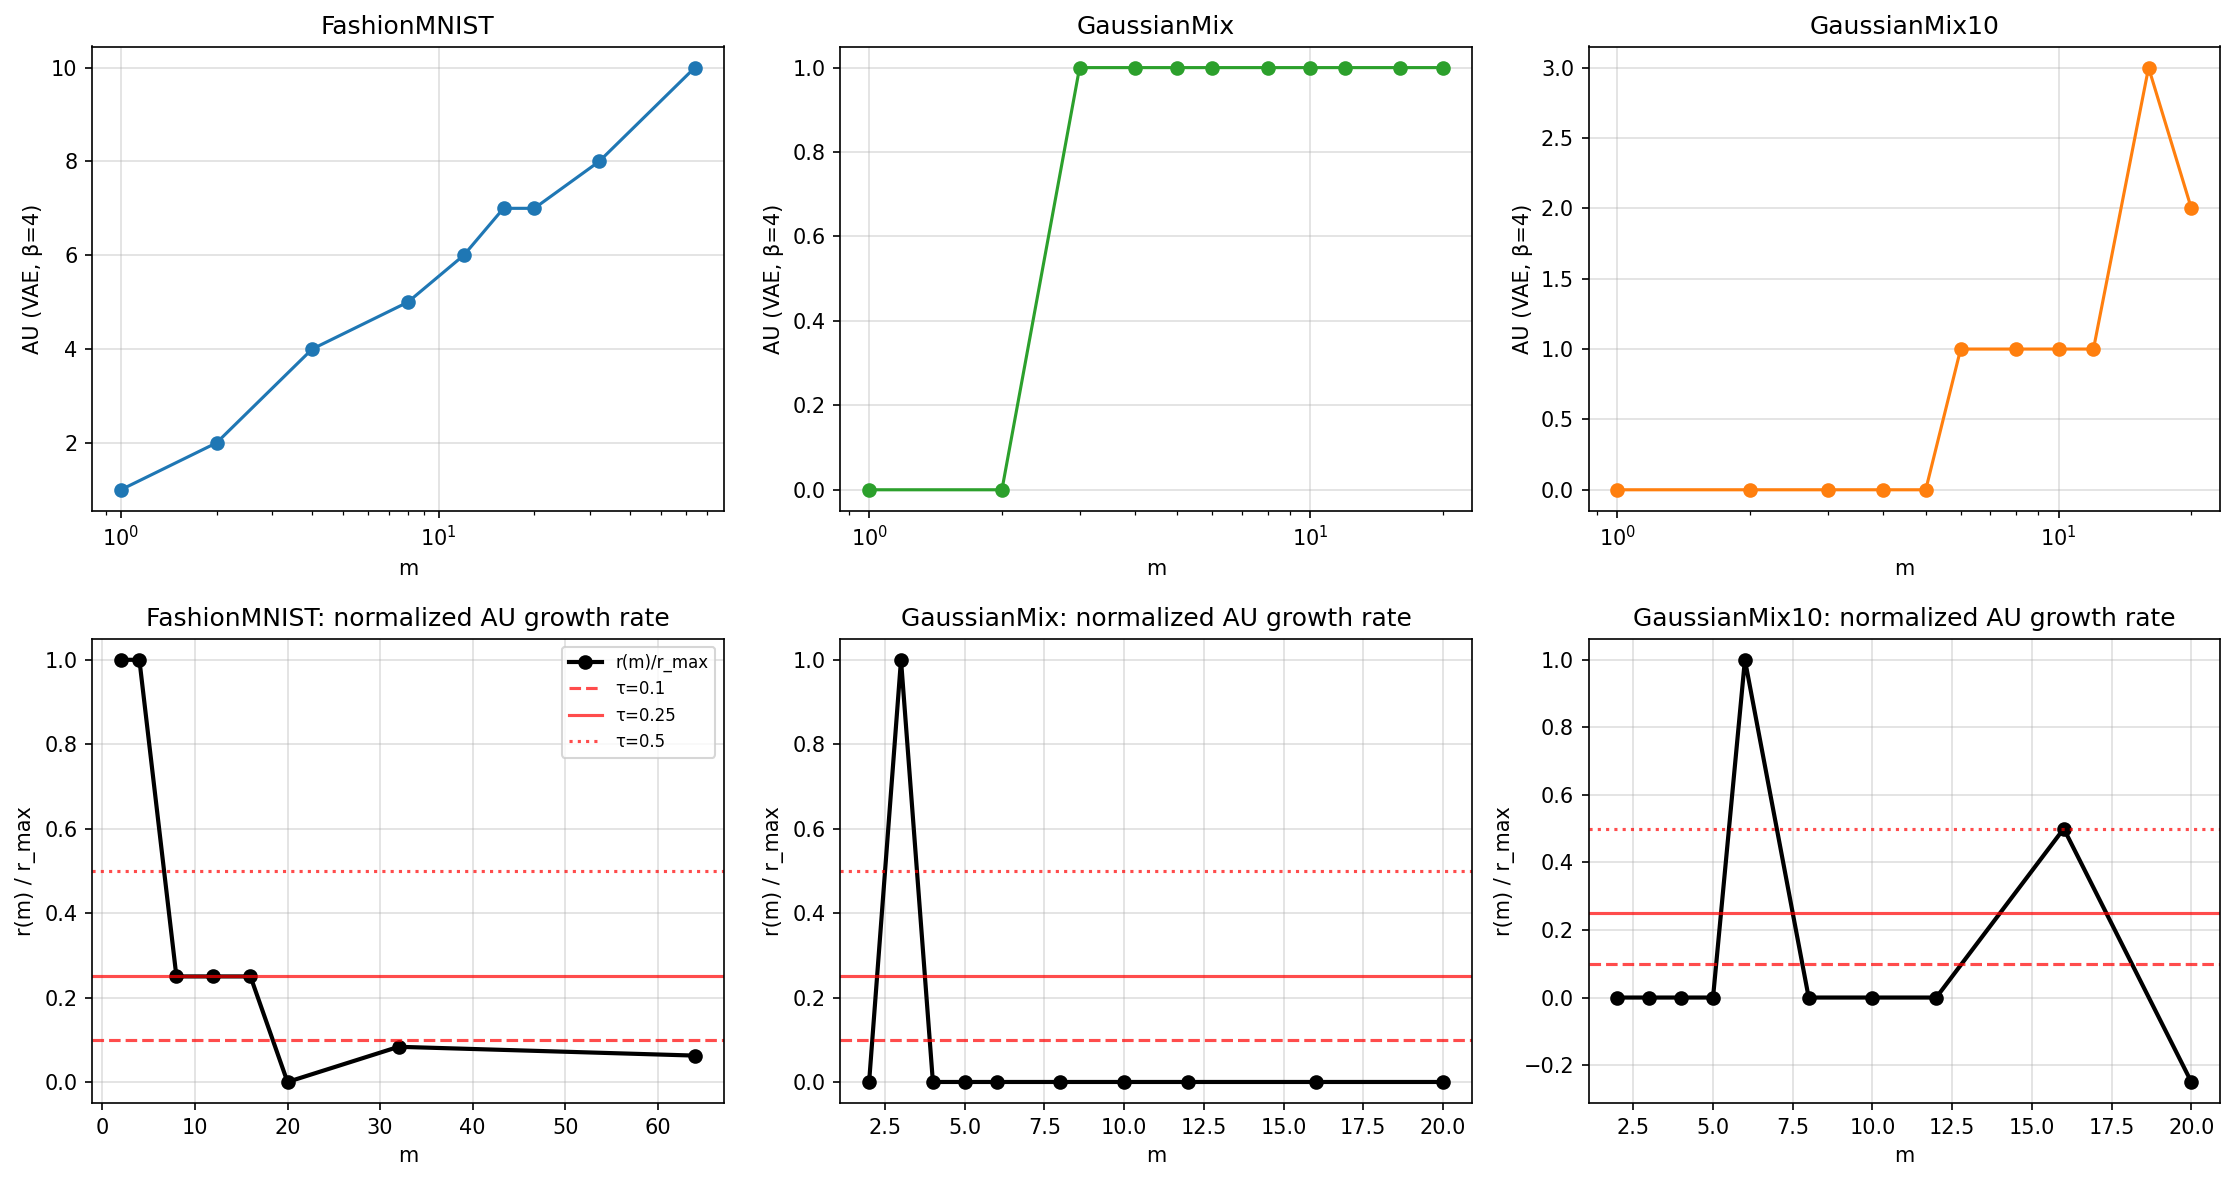
\includegraphics[width=0.98\linewidth]{results/figures/EZ_tau_robustness.png}
\caption{実験 EZ：各データセットの AU 増加プロファイル（上段）と正規化 AU 増加率$r(m)/r_\mathrm{max}$（下段）．
赤線は$\tau = 0.1$（破線），$\tau = 0.25$（実線），$\tau = 0.5$（点線）を示す．
Fashion-MNIST は漸増型（MNIST と同類），Gaussian 混合は$[0,1]$正規化の影響で事後分布崩壊が生じ AU が低い．}
\label{fig:ez_tau}
\end{figure}

\end{document}
